% \chude{GIÁ TRỊ LỚN NHẤT, GIÁ TRỊ NHỎ NHẤT LIÊN QUAN ĐẾN MẶT PHẲNG}
\begin{dang}{GIÁ TRỊ LỚN NHẤT, GIÁ TRỊ NHỎ NHẤT LIÊN QUAN ĐẾN BIỂU THỨC}
	\begin{bt}%[2H5C1-5]
		Trong KG $Oxyz$, cho các điểm $A_1$, $A_2,\ldots$, $A_n$ và mặt phẳng $(P)\colon Ax+By+Cz+D=0$. Tìm tọa độ điểm $M(x_0 ; y_0 ; z_0)$ thuộc mặt phẳng $(P)$ sao cho $T=\left|\alpha_1 \vec{M A_1}+\alpha_2 \vec{M A_2}+\ldots+\alpha_n \vec{M A_n}\right|$ nhỏ nhất (với $\alpha_1$; $\alpha_2$;$\ldots$; $\alpha_n$ là các số thực cho trước thỏa mãn $\alpha_1+\alpha_2+\ldots+\alpha_n \neq 0$).
		\loigiai{
			\begin{itemize}
				\item \textit{Cách 1: Phương pháp hình học (Chọn điểm phụ)}
				\begin{itemize}
					\item \textit{Bước 1:} Tìm tọa độ điểm phụ $I$.\\
					Gọi $I$ là điểm thỏa mãn $\alpha_1 \vec{I A_1}+\alpha_2 \vec{I A_2}+\ldots+\alpha_n \vec{I A_n}=\vec{0}$.\\
					Dựa vào đẳng thức $\alpha_1 \vec{I A_1}+\alpha_2 \vec{I A_2}+\ldots+\alpha_n \vec{I A_n}=\vec{0}$ ta tìm được tọa độ điểm $I$.\\
					Ta có
					\begin{eqnarray*}
						& & \alpha_1\left(\vec{M I}+\vec{I A_1}\right)+\alpha_2\left(\vec{M I}+\vec{I A_2}\right)+\ldots+\alpha_n\left(\vec{M I}+\vec{I A_n}\right) \\
						&= & \left(\alpha_1+\alpha_2+\ldots+\alpha_n\right) \vec{M I}+\alpha_1 \vec{I A_1}+\alpha_2 \vec{I A_2}+\ldots+\alpha_n \vec{I A_n} \\
						&= & \left(\alpha_1+\alpha_2+\ldots+\alpha_n\right) \vec{M I} \quad\left(\text { do } \alpha_1 \vec{I A_1}+\alpha_2 \vec{I A_2}+\ldots+\alpha_n \vec{I A_n}=\vec{0}\right) \\
						\Rightarrow T&= & \left|\alpha_1 \vec{M A_1}+\alpha_2 \vec{M A_2}+\ldots+\alpha_n \vec{M A_n}\right|\\
						&=&\left|\alpha_1+\alpha_2+\ldots+\alpha_n\right||\vec{M I}|.
					\end{eqnarray*}
					Vì $\alpha_1+\alpha_2+\ldots+\alpha_n$ là hằng số khác không nên $T_{\min } \Leftrightarrow|\vec{M I}|_{\min }$.\\
					Mà $M \in(P)$ nên $MI$ nhỏ nhất khi điểm $M$ cần tìm là hình chiếu của $I$ trên mặt phẳng $(P)$.
					\item \textit{Bước 2:} Tìm tọa độ điểm $M$.\\
					Lập PTTS đường thẳng $I M$ với $\heva{&\text{qua } I \\&\vec{u}_{I M}=\vec{n}_P=(A ; B ; C).}$\\
					Ta có $M=I M \cap (P) \Rightarrow$ tọa độ điểm $M$ cần tìm.
				\end{itemize}
				\item \textit{Cách 2: Phương pháp đại số}\\
				Dùng bất đẳng thức bộ $3$ của Bunhiacốpxki.\\
				Với $a$, $b$, $c$, $x$, $y$, $z$ $\in \mathbb{R}$, ta có
				\[(a x+b y+c z)^2  \leq(a^2+b^2+c^2)(x^2+y^2+z^2).\]
				Dấu \lq\lq =\rq\rq\,xảy ra khi $\dfrac{a}{x}=\dfrac{b}{y}=\dfrac{c}{z}.$
			\end{itemize}	
		}
	\end{bt}
	
	\begin{bt}%[2H5C1-5]
		Trong KG $Oxyz$, cho các điểm $A_1$, $A_2$,$\ldots$, $A_n$ và mặt phẳng $(P)\colon Ax+By+Cz+D=0$. Tìm tọa độ điểm $M(x_0 ; y_0 ; z_0)$ thuộc mặt phẳng $(P)$ sao cho $T=\alpha_1 M A_1^2+\alpha_2 M A_2^2+\ldots+\alpha_n M A_n^2$ nhỏ nhất (hoặc lớn nhất) (với $\alpha_1 ; \alpha_2 \ldots \alpha_n$ là các số thực cho trước thỏa mãn $\alpha_1+\alpha_2+\ldots+\alpha_n \neq 0$).\\
		\textbf{Chú ý:}
		\begin{align*}
			& T_{\min } \Leftrightarrow \alpha_1+\alpha_2+\ldots+\alpha_n>0 \\
			& T_{\max } \Leftrightarrow \alpha_1+\alpha_2+\ldots+\alpha_n<0
		\end{align*}
		\loigiai{
			\begin{itemize}
				\item \textit{Cách 1: Phương pháp hình học (Chọn điểm phụ)}
				\begin{itemize}
					\item \textit{Bước 1:} Tìm tọa độ điểm phụ $I$.\\
					Gọi $I$ là điểm thỏa mãn $\alpha_1\vec{IA_1}+\alpha_2\vec{IA_2}+\ldots+\alpha_n\vec{IA_n}=\vec{0}$.\\
					Dựa vào đẳng thức $\alpha_1 \vec{I A_1}+\alpha_2 \vec{I A_2}+\ldots+\alpha_n \vec{I A_n}=\vec{0}$ ta tìm được tọa độ điểm $I$.\\
					Ta có
					\begin{eqnarray*}
						T& & \alpha_1 M A_1^2+\alpha_2 M A_2^2+\ldots+\alpha_n M A_n^2 \\
						&= & \alpha_1\left(\vec{M A_1}\right)^2+\alpha_2\left(\vec{M A_2}\right)^2+\ldots+\alpha_n\left(\vec{M A_n}\right)^2 \\
						&= & \alpha_1\left(\vec{M I}+\vec{I A_1}\right)^2+\alpha_2\left(\vec{M I}+\vec{I A_2}\right)^2+\ldots+\alpha_n\left(\vec{M I}+\vec{I A_n}\right)^2 \\
						&= & \left(\alpha_1+\alpha_2+\ldots+\alpha_n\right) M I^2+\alpha_1 I A_1^2+\alpha_2 I A_2^2+\ldots+\alpha_n I A_n^2+2 \vec{M I} \\
						&= & \left(\alpha_1+\alpha_2+\ldots+\alpha_n\right) \vec{M I}+\alpha_1 I A_1^2+\alpha_2 I A_2^2+\ldots+\alpha_n I A_n^2\\
						\Rightarrow T&= & \left(\alpha_1+\alpha_2+\ldots+\alpha_n\right) \vec{M I}+\alpha_1 I A_1^2+\alpha_2 I A_2^2+\ldots+\alpha_n I A_n^2.
					\end{eqnarray*}
					Vì  $\alpha_1 I A_1^2+\alpha_2 I A_2^2+\ldots+\alpha_n I A_n^2$ không đổi nên
					\begin{itemize}
						\item Với $\alpha_1+\alpha_2+\ldots+\alpha_n>0$ thì $T$ đạt giá trị nhỏ nhất khi và chỉ khi $M I$ nhỏ nhất.
						\item Với $\alpha_1+\alpha_2+\ldots+\alpha_n<0$ thì $T$ đạt giá trị lớn nhất khi và chỉ khi $M I$ nhỏ nhất.
					\end{itemize}
					Mà $M \in(P)$ nên $M I$ nhỏ nhất khi điểm $M$ cần tìm là hình chiếu của $I$ trên mặt phẳng $(P)$
					\item \textit{Bước 2:} Tìm tọa độ điểm $M$.\\
					Lập PTTS đường thẳng $I M$ với $\heva{& \text{qua } I \\& \vec{u}_{I M}=\vec{n}_P=(A ; B ; C).}$\\
					Ta có $M=I M \cap(P) \Rightarrow$ tọa độ điểm $M$ cần tìm.
				\end{itemize}
				\item \textit{Cách 2: Phương pháp đại số}\,\\
				Dùng bất đẳng thức bộ $3$ của Bunhiacốpxki.\\
				Với $a$, $b$, $c$, $x$, $y$, $z \in \mathbb{R}$, ta có 
				\[(a x+b y+c z)^2 \leq(a^2+b^2+c^2)(x^2+y^2+z^2).\]
				Dấu \lq\lq=\rq\rq\,xảy ra $\Leftrightarrow \dfrac{a}{x}=\dfrac{b}{y}=\dfrac{c}{z}$.
			\end{itemize}
		}
	\end{bt}
\end{dang}
\TN
\Opensolutionfile{ans}[ans/ans-C5B3CD5-LC]
\begin{ex}%[2H5C1-5]
		Trong KG $Oxyz$, cho hai điểm $A(1 ; 0 ; 2)$, $B(3 ; 1 ;-1)$ và mặt phẳng $(P)\colon x+y+z-1=0$. Gọi $M(a ; b ; c) \in(P)$ sao cho $\left|3 \vec{M A}-2 \vec{M B}\right|$ đạt giá trị nhỏ nhất. Tính $S=9a+3b+6c$.
		\choice
		{$4$}
		{\True $3$}
		{$2$}
		{$1$}
	\loigiai{
	\begin{itemize}
		\item \textit{Cách 1: Phương pháp hình học}\,\\
			Gọi $I(m ; n ; p)$ là điểm thỏa mãn  $3 \vec{I A}-2 \vec{I B}=\vec{0}$.\\
			Ta có $\vec{I A}=(1-m ;-n ; 2-p)$; $\vec{I B}=(3-m ; 1-n ;-1-p)$.
			\[3 \vec{I A}-2 \vec{I B}=\vec{0} \Leftrightarrow\heva{
				&3(1-m)-2(3-m)=0\\
				&3(-n)-2(1-n)=0\\
				&3(2-p)-2(-1-p)=0}
			 \Leftrightarrow \heva{&m=-3 \\&n=-2\\&p=8} \Rightarrow I(-3 ;-2 ; 8).\]
		Lại có $\left|3\vec{MA}-2\vec{MB}\right|=\left|3\left(\vec{MI}+\vec{IA}\right)-2\left(\vec{MI}+\vec{IB}\right)\right|=\left|\vec{MI}\right|=MI$.\\
		Khi đó, $\left|3\vec{MA}-2\vec{MB}\right|$ đạt giá trị nhỏ nhất, $M \in(P)$.\\
		Hay $ MI$ nhỏ nhất, $M \in(P)$.\\
		Khi đó $M$ là hình chiếu vuông góc của $I$ trên $(P)$.\\
		Gọi $\Delta$ là đường thẳng qua $I$ và vuông góc với $(P)$. Khi đó $\Delta$ nhận véc-tơ pháp tuyến của $(P)$ là $\vec{n}=(1 ; 1 ; 1)$  làm véc-tơ chỉ phương.\\
		Suy ra phương trình $\Delta$ có dạng $\Delta\colon \heva{&x=-3+t \\&y=-2+t \\&z=8+t.}$\\
		Tọa độ $M$ là nghiệm của hệ\\
		$$\heva{
				&x=-3+t\\
				&y=-2+t\\
				&z=8+t\\
				&x+y+z-1=0}
			\Leftrightarrow\heva{
				&t=-\dfrac{2}{3}\\
				&x=-\dfrac{11}{3}\\
				&y=-\dfrac{8}{3}\\
				&z=\dfrac{22}{3}}
				\Rightarrow\heva{
				&a=-\dfrac{11}{3}\\
				&b=-\dfrac{8}{3}\\
				&c=\dfrac{22}{3}}
				\Rightarrow S=9a+3b+6c=3.
		$$
	\item \textit{Cách 2: Phương pháp đại số}\,\\
	$M(a ; b ; c) \in(P) \Rightarrow a+b+c-1=0.$
	\begin{eqnarray*}
		& & 3 \vec{M A}-2 \vec{M B}=(-3-a ;-2-b ; 8-c)\\
		&\Leftrightarrow & |3 \vec{M A}-2 \vec{M B}|=\sqrt{(a+3)^2+(b+2)^2+(c-8)^2}
	\end{eqnarray*}
		Ta có $a+b+c-1=0 \Leftrightarrow(a+3)+(b+2)+(c-8)=-1$.
		\begin{eqnarray*}
			|(a+3)+(b+2)+(c-8)|
			&=& 1 \cdot(a+3)+1 \cdot(b+2)+1 \cdot(c-8)| \\
			&\leq & \sqrt{\left(1^2+1^2+1^2\right)\left[(a+3)^2+(b+2)^2+(c-8)^2\right]} \\
			\Rightarrow \sqrt{(a+3)^2+(b+2)^2+(c-8)^2} &\geq& \dfrac{1}{\sqrt{3}}.
		\end{eqnarray*}
		Dấu \lq\lq=\rq\rq\,xảy ra $\dfrac{a+3}{1}=\dfrac{b+2}{1}=\dfrac{c-8}{1} \Leftrightarrow a+3=b+2=c-8 \Leftrightarrow\heva{&a-b=-1 \\& a-c=-11.}$\\
		Ta có hệ $\heva{&a-b=-1 \\&a-c=-11 \\& a+b+c-1=0} \Leftrightarrow\heva{&a=-\dfrac{11}{3} \\&b=-\dfrac{8}{3} \\&c=\dfrac{22}{3}}\Rightarrow S=9a+3b+6c=3.$		
	\end{itemize}
	}
\end{ex}
%4-6

%%%=============EX_2=============%%%
\begin{ex}%[2H2C2-2]
	Trong KG $Oxyz$, cho ba điểm $A(4;2; 2)$, $B(1;1;-1)$, $C(2;-2;-2)$. Tìm tọa độ điểm $M$ thuộc $(Oxy)$ sao cho $\left|\vec{MA}+2\vec{MB}-\vec{MC}\right|$ nhỏ nhất.
	\choice
	{\True $M(2;3;0)$}
	{$M(1;3;0)$}
	{$M(2;-3;0)$}
	{$M(2;3;1)$} 
	\loigiai{
		\begin{enumerate}[\bf Cách 1.]
			\item Phương pháp hình học.\\
			Gọi $I$ là điểm thỏa mãn $\vec{IA}+2\vec{IB}-\vec{IC}=\vec{0}$.\\
			Ta có \begin{eqnarray*}
				\bullet&&\vec{IA}+2\vec{IB}-\vec{IC}=\vec{0}\\
				&\Leftrightarrow& \vec{IO}+\vec{OA}+2\left(\vec{IO}+\vec{OB}\right)-\left(\vec{IO}+\vec{OC}\right)=\vec{0}\\
				&\Leftrightarrow& \vec{OI}=\dfrac{1}{2} (\vec{OA}+2\vec{OB}-\vec{OC})\Rightarrow I(2;3;1).\\
				\bullet&& \left|\vec{MA}+2\vec{MB}-\vec{MC}\right|=\left|2\vec{MI}+\vec{IA}+2\vec{IB}-\vec{IC}\right|=2\cdot MI.
			\end{eqnarray*}
			$\left|\vec{MA}+2\vec{MB}-\vec{MC}\right|$ nhỏ nhất $\Leftrightarrow$ $MI$ nhỏ nhất $\Leftrightarrow$ $M$ là hình chiếu của $I$ trên mp$(Oxy)$.\\
			Vì $I(2;3;1)\Rightarrow M(2;3;0)$.
			\item Phương pháp hình học.
			\begin{center}
				\begin{tikzpicture}
					\def\a{4}
					\path 	(0:0) coordinate (A)
					++(0:\a) coordinate (B)
					++(-140:.5*\a) coordinate (C)
					($(A)!.5!(B)$) coordinate (D)
					($(A)!.5!(C)$) coordinate (E)
					($(D)+(120:.5*\a)$) coordinate (M)
					($(M)!.5!(E)$) coordinate (F)
					(intersection of A--B and M--E) coordinate (G);
					\draw[dashed] 	(G)--(D);
					\draw	(G)--(A)--(C)--(B)--(D)	(D)--(M)--(E)--cycle	(D)--(F);
					\foreach \x/\g in {A/180,B/0,C/-45,D/45,E/-100,F/175,M/90}
					\fill[black] 	(\x) circle (1pt)
					($(\g:3mm)+(\x)$) node {$\x$};
				\end{tikzpicture}
			\end{center}
			Gọi $D$; $E$; $F$ lần lượt là trung điểm của $AB$; $AC$; $ME$.\\
			Ta có
			\begin{eqnarray*}
				\left|\vec{MA}+2\vec{MB}-\vec{MC}\right|&=&\left|\vec{MA}+\vec{MB}+\vec{MB}-\vec{MC}\right|\\
				&=&\left|2\cdot \vec{MD}+\vec{CB}\right|\\
				&=&\left|2\cdot \vec{MD}+2\cdot \vec{ED}\right|\\
				&=&2\left|2\cdot \vec{FD}\right|\\
				&=&4\cdot FD.
			\end{eqnarray*}
			Ta lại có 
			\begin{itemize}
				\item $M(x;y;0)$, $D\left(\dfrac{5}{2};\dfrac{3}{2};\dfrac{1}{2}\right)$, $E(3;0;0)$, $F\left(\dfrac{x+3}{2};\dfrac{y}{2};0\right)$;
				\item $FD_{\min} \Leftrightarrow$ $F$ là hình chiếu của $D$ trên mp$(Oxy)\Leftrightarrow \heva{&x=2\\&y=3}\Leftrightarrow M(2;3;0)$.
			\end{itemize}
			\item Phương pháp đại số.\\
			$M\in (Oxy)\Rightarrow M(x;y;0)$;
			\begin{eqnarray*}
				\vec{MA}+2\vec{MB}-\vec{MC}&=&(4-2x;6-2y;-1)\\
				\Rightarrow \left|\vec{MA}+2\vec{MB}-\vec{MC}\right|&=&\sqrt{\left(4-2x\right)^2+\left(6-2y\right)^2+1}\\
				& \ge & 1.
			\end{eqnarray*}
			Dấu \lq\lq$=$\rq\rq, xảy ra $\Leftrightarrow x=2$; $y=3$. Khi đó $M(2;3;0)$.
			\item Trắc nghiệm, thay đáp án.\\
			$M\in (Oxy)\Rightarrow M(x;y;0)$. Ta có
			\begin{eqnarray*}
				\vec{MA}+2\vec{MB}-\vec{MC}&=&(4-2x;6-2y;-1)\\
				\Rightarrow \left|\vec{MA}+2\vec{MB}-\vec{MC}\right|&=&\sqrt{(4-2x)^2+(6-2y)^2+1}.
			\end{eqnarray*}
			\begin{itemize}
				\item Thế tọa độ điểm $M(2;3;0)$ vào ta được $\left|\vec{MA}+2\vec{MB}-\vec{MC}\right|=1$.
				\item Thế tọa độ điểm $M(1;3;0)$ vào ta được $\left|\vec{MA}+2\vec{MB}-\vec{MC}\right|=\sqrt{17}$.
				\item Thế tọa độ điểm $M(2;-3;0)$ vào ta được $\left|\vec{MA}+2\vec{MB}-\vec{MC}\right|=\sqrt{145}$.
				\item Điểm $M(2;3;1)$ không thuộc $\left(Oxy\right)$ nên bị loại.
			\end{itemize}
		\end{enumerate}
	}
\end{ex}

%%%=============EX_3=============%%%
\begin{ex}%[2H2C2-2]
	Trong hệ trục $Oxyz$, cho điểm $A(-1;3;5)$, $B(2;6;-1)$, $C(-4;-12;5)$ và mặt phẳng $(P)\colon x+2y-2z-5=0$. Gọi $M$ là điểm di động trên $(P)$. Gía trị nhỏ nhất của biểu thức $S=\left|\vec{MA}+\vec{MB}+\vec{MC}\right|$ là 
	\choice
	{$42$}
	{\True $14$}
	{$14\sqrt{3}$}
	{$\dfrac{14}{\sqrt{3}}$}
	\loigiai{
		Gọi $G\left(x_1;y_1;z_1 \right)$ là trọng tâm tam giác $ABC$.\\
		Vì $G$ là trọng tâm tam giác $ABC$ và $M$ là điểm tùy ý nên $\vec{MA}+\vec{MB}+\vec{MG}=3\vec{MG}$.\\
		Vậy $S=\left|\vec{MA}+\vec{MB}+\vec{MC}\right|=\left|3\vec{MG}\right|=3MG$.\\
		Do $G$ là trọng tâm $\triangle ABC$ nên $\heva{&{x_1=\dfrac{x_A+x_B+x_C}{3}=\dfrac{-1+2-4}{3}=-1} \\
			&{y_1=\dfrac{y_A+y_B+y_C}{3}=\dfrac{3+6-12}{3}=-1} \\
			&{z_1=\dfrac{z_A+z_B+z_C}{3}=\dfrac{5-1+5}{3}=3}
			&} \Rightarrow G(-1;-1;3)$.\\
		Vì $G$ cố định nên $S=3MG$ đạt giá trị nhỏ nhất khi và chỉ khi $MG$ nhỏ nhất. \\
		Tức là $MG\perp (P)$.\\
		Ta có $\mathrm{d}\big(G,(P)\big)=\dfrac{\left|-1\cdot 1+2\cdot(-1)-2\cdot 3-5\right|}{\sqrt{1^2+2^2+(-2)^2}}=\dfrac{14}{3}=MG$.\\
		Vậy giá trị nhỏ nhất $S=\left|\vec{MA}+\vec{MB}+\vec{MC}\right|=\left|3\vec{MG}\right|=3MG=3\cdot\dfrac{14}{3}=14$.
	}
\end{ex}

%%%=============EX_4=============%%%
\begin{ex}%[2H2C2-2]
	Trong KG $Oxyz$, cho ba điểm $A(4;2;2)$, $B(1;1;-1)$, $C(2;-2;-2)$. Tìm tọa độ điểm $M$ thuộc mặt phẳng $(Oyz)$ sao cho $\left|\vec{MA}+2\vec{MB}-\vec{MC}\right|$ nhỏ nhất
	\choice
	{$M(2; 3; 1)$}
	{\True $M(0; 3; 1)$}
	{$M(0;-3; 1)$}
	{$M(0; 1; 2)$}
	\loigiai{
		Gọi $I(x; y; z)$ là điểm thỏa $\vec{IA}+2\vec{IB}-\vec{IC}=\vec0$.\\
		Khi đó 
		\begin{eqnarray*}
			& &\vec{IA}+2\vec{IB}-\vec{IC}=\vec{0}\\
			&\Leftrightarrow& \big(\vec{OA}-\vec{OI}\big)+2\big(\vec{OB}-\vec{OI}\big)-\big(\vec{OC}-\vec{OI}\big)=\vec{0}\\
			&\Leftrightarrow& \vec{OI}=\dfrac{1}{2} \big(\vec{OA}+2\vec{OB}-\vec{OC}\big)=(2; 3; 1)\Rightarrow I(2; 3; 1).
		\end{eqnarray*}
		Ta có
		\begin{eqnarray*}
			\left|\vec{MA}+2\vec{MB}-\vec{MC}\right|&=&\left|(\vec{MI}+\vec{IA})+2(\vec{MI}+\vec{IB})-(\vec{MI}+\vec{IC})\right|\\
			&=&\left|2\vec{MI}+\vec{IA}+2\vec{IB}-\vec{IC}\right|\\
			&=&2\left|\vec{MI}\right|=2MI.
		\end{eqnarray*}
		$\left|\vec{MA}+2\vec{MB}-\vec{MC}\right|$ nhỏ nhất khi và chỉ khi $MI$ ngắn nhất.\\
		Khi đó $M$ là hình chiếu của $I(2; 3; 1)$ lên mặt phẳng $(Oyz)$. \\
		Suy ra $M(0; 3; 1)$. 
	}
\end{ex}

%%%=============EX_5=============%%%
\begin{ex}%[2H2C2-2]
	Trong KG $Oxyz$, cho các điểm $A(1;-1;3)$, $B(2;1;0)$, $C(-3;-1;-3)$ và mặt phẳng $(P)\colon x+y-z-4=0$. Gọi $M(a,b,c)$ là điểm thuộc mặt phẳng $(P)$ sao cho biểu thức $T=\left|3\vec{MA}-2\vec{MB}+\vec{MC}\right|$ đạt giá trị nhỏ nhất. Tính giá trị của biểu thức $S=a+b+c$. 
	\choice
	{$S=3$}
	{$S=-1$}
	{\True $S=2$}
	{$S=1$}
	\loigiai{
		Gọi $I(x;y;z)$ là điểm thỏa mãn $3\vec{IA}-2\vec{IB}+\vec{IC}=\vec{0}$.\\
		Ta có 
		\begin{itemize}
			\item $\vec{IA}=(1-x;-1-y;3-z)\Rightarrow 3\vec{IA}=(3-3x;-3-3y;9-3z)$.
			\item $\vec{IB}=(2-x;1-y;-z)\Rightarrow 2\vec{IB}=(4-2x;2-2y;-2z)$.
			\item $\vec{IC}=(-3-x;-1-y;-3-z)$.
		\end{itemize}
		Khi đó 
		\begin{eqnarray*}
			& &3\vec{IA}-2\vec{IB}+\vec{IC}=(-2x-4;-2y-6;-2z+6)=\vec{0}\\
			&\Leftrightarrow& \heva{&-2x-4=0\\&-2y-6=0\\&-2z+6=0}\Leftrightarrow \heva{&x=-2\\&y=-3\\&z=3.}
		\end{eqnarray*}
		Vậy $I(-2;-3;3)$.\\
		Ta có
		\begin{eqnarray*}
			T&=&\left|3\vec{MA}-2\vec{MB}+\vec{MC}\right|\\
			&=&\left|3(\vec{MI}+\vec{IA})-2(\vec{MI}+\vec{IB})+(\vec{MI}+\vec{IC})\right|\\
			&=&2\left|\vec{MI}\right|.
		\end{eqnarray*}
		Suy ra $T_{\min} \Leftrightarrow \left|\vec{MI}\right|_{\min}$ khi và chỉ khi $M$ là hình chiếu của $I$ lên mặt phẳng $(P)$.\\
		Đường thẳng $MI$ đi qua $I(-2;-3;3)$ và vuông góc với mặt phẳng $(P)$ có PTTS là $MI\colon \heva{&x=-2+t\\&y=-3+t\\&z=3-t.}$\\
		Lấy $M(-2+t;-3+t;3-t)\in MI$.\\
		Mặt khác $M\in (P)\Rightarrow (-2+t)+(-3+t)-(3-t)-4=0\Rightarrow t=4$. Suy ra $M(2;1;-1)$.\\
		Vậy $a+b+c=2$ 
	}
\end{ex}
\begin{ex}%[2H5C1-5]
	Trong không gian $O x y z$ cho mặt phẳng $(P)\colon x+y+z-3=0$ và ba điểm $A(3; 1; 1), B(7; 3; 9)$ và $C(2; 2; 2)$. Điểm $M(a; b; c)$ trên $(P)$ sao cho $|\overrightarrow{MA}+2 \overrightarrow{MB}+3 \overrightarrow{MC}|$ đạt giá trị nhỏ nhất. Tính $2a-10b+c$.
	\choice
	{\True$\dfrac{62}{9}$}
	{$\dfrac{27}{9}$}
	{$\dfrac{46}{9}$}
	{$\dfrac{43}{9}$}	
	\loigiai{
		\begin{itemize}
			\item Gọi $I(x; y; z)$ là điểm thỏa mãn $\overrightarrow{IA}+2 \overrightarrow{IB}+3 \overrightarrow{I C}=\overrightarrow{0}$.\\
			Ta có $\heva{&\overrightarrow{I A}=(3-x; 1-y; 1-z) \\& \overrightarrow{I B}=(7-x; 3-y; 9-z) \\& \overrightarrow{I C}=(2-x; 2-y; 2-z).}$\\
			\item $\overrightarrow{I A}+2 \overrightarrow{I B}+3 \overrightarrow{I C}=\overrightarrow{0} \Leftrightarrow\heva{& 
				{2 3-6 x=0} \\&
				{1 3-6 y=0} \\&
				{2 5-6 z=0}
			} \Leftrightarrow \heva{&
				x=\dfrac{23}{6} \\&
				y=\dfrac{13}{6} \\&
				z=\dfrac{25}{6}.
			}$\\
			Suy ra
			$I\left(\dfrac{23}{6}; \dfrac{13}{6}; \dfrac{25}{6}\right).\\
			|\overrightarrow{MA}+2 \overrightarrow{MB}+3 \overrightarrow{MC}|=|6 \overrightarrow{MI}+(\overrightarrow{IA}+2 \overrightarrow{IB}+3 \overrightarrow{IC})|=|6 \overrightarrow{MI}|=6 MI.$\\
			$|\overrightarrow{M A}+2 \overrightarrow{M B}+3 \overrightarrow{M C}|$ đạt giá trị nhỏ nhất $\Leftrightarrow M$ là hình chiếu của $I$ lên mặt phẳng $(P)$.
			\item Gọi đường thẳng $(d)$ đi qua $I$ và vuông góc $(P)$.
			Ta có $(d)$ đi qua $I\left(\dfrac{23}{6}; \dfrac{13}{6}; \dfrac{25}{6}\right)$ và nhận $\overline{n_p}=(1; 1; 1)$ làm vectơ chỉ phương.\\
			Suy ra phương trình $(d)\colon\heva{&x=\dfrac{23}{6}+t \\& y=\dfrac{13}{6}+t \\& z=\dfrac{25}{6}+t.}$\\
			$M \in(d) \Leftrightarrow M\left(\dfrac{23}{6}+t; \dfrac{13}{6}+t; \dfrac{25}{6}+t\right)$.\\
			$M \in(P) \Leftrightarrow \dfrac{23}{6}+t+\dfrac{13}{6}+t+\dfrac{25}{6}+t-3=0 \Leftrightarrow t=\dfrac{-43}{18} \Leftrightarrow M\left(\dfrac{13}{9}; \dfrac{-2}{9}; \dfrac{16}{9}\right)$.\\
			Do đó $\heva{&a=\dfrac{13}{9} \\& b=\dfrac{-2}{9} \\& c=\dfrac{16}{9}} \Rightarrow 2 a-10 b+c=\dfrac{62}{9}$.
		\end{itemize}
	}
\end{ex}

\begin{ex}%[2H5C1-5]
	Trong KG $Oxyz$, cho ba điểm $A\left(1;1;1 \right),B\left(-1;2;0 \right),C\left(3;-1;2 \right)$ và điểm $M$ thuộc mặt phẳng $(\alpha)\colon2x-y+2z+7=0$. Tính giá trị nhỏ nhất của $\break P=\left| 3\overrightarrow{MA}+5\overrightarrow{MB}-7\overrightarrow{MC} \right|$.
	\choice
	{${{P}_{\min}}=20$}
	{${{P}_{\min}}=5$}
	{${{P}_{\min}}=25$}
	{\True${{P}_{\min}}=27$}
	\loigiai{
		Gọi $I$ là điểm thỏa mãn
		\begin{eqnarray*}
			&& 3\overrightarrow{IA}+5\overrightarrow{IB}-7\overrightarrow{IC}=\overrightarrow{0}\\
			&\Leftrightarrow&3\left(\overrightarrow{OA}-\overrightarrow{OI} \right)+5\left(\overrightarrow{OB}-\overrightarrow{OI} \right)-7\left(\overrightarrow{OC}-\overrightarrow{OI} \right)=\overrightarrow{0}\\
			&\Leftrightarrow&\overrightarrow{OI}=3\overrightarrow{OA}+5\overrightarrow{OB}-7\overrightarrow{OC}.
		\end{eqnarray*}
		Suy ra tọa độ điểm $I=\left(-23;20;-11 \right).$\\
		Khi đó 
		\begin{eqnarray*}
			\overrightarrow{u}&=&3\overrightarrow{MA}+5\overrightarrow{MB}-7\overrightarrow{MC}\\
			&=&3\left(\overrightarrow{IA}-\overrightarrow{IM} \right)+5\left(\overrightarrow{IB}-\overrightarrow{IM} \right)-7\left(\overrightarrow{IC}-\overrightarrow{IM} \right)\\
			&=&-\overrightarrow{IM}+\left(3\overrightarrow{IA}+5\overrightarrow{IB}-7\overrightarrow{IC} \right)\\
			&=&-\overrightarrow{IM}.
		\end{eqnarray*}
		Nên $P=\left| 3\overrightarrow{MA}+5\overrightarrow{MB}-7\overrightarrow{MC} \right|$ ${=\left|-\overrightarrow{IM} \right|}$ $=IM$ $\ge d\left(I,(\alpha) \right)$.\\
		Vậy ${{P}_{\min}}=d\left(I,(\alpha) \right)$ $=\dfrac{\left| 2\cdot\left(-23 \right)-20+2\cdot\left(-11 \right)+7 \right|}{\sqrt{{{2}^2}+{{1}^2}+{{2}^2}}}=27$.
	}
\end{ex}


\begin{ex}%[2H5C1-5]
	Trong không gian với hệ trục tọa độ ${Oxyz}$, cho bốn điểm ${A\left(2;-3;7 \right)}$, ${B\left(0;4;1 \right)}$, ${C\left(3;0;5 \right)}$ và ${D\left(3;3;3 \right)}$. Gọi ${M}$ là điểm nằm trên mặt phẳng ${\left(Oyz \right)}$ sao cho biểu thức ${\left| \overrightarrow{MA}+\overrightarrow{MB}+\overrightarrow{MC}+\overrightarrow{MD} \right|}$ đạt giá trị nhỏ nhất. Khi đó tọa độ của ${M}$ là
	\choice
	{$M(0;1;-4)$}
	{$M(2;1;0)$}
	{$M(0;1;-2)$}
	{\True$M(0;1;4)$}
	\loigiai{
		Ta có ${\overrightarrow{AB}=\left(-2;7;-6 \right)}$, ${\overrightarrow{AC}=\left(1;3;-2 \right)}$, ${\overrightarrow{AD}=\left(1;6;-4 \right)}$ nên ${\left[\overrightarrow{AB},\overrightarrow{AC} \right]\cdot\overrightarrow{AD}=-4\ne 0}$.
		Suy ra ${\overrightarrow{AB}}$, ${\overrightarrow{AC}}$, ${\overrightarrow{AD}}$ không đồng phẳng.\\
		Gọi ${G}$ là trọng tâm tứ diện ${ABCD}$. Khi đó ${G\left(2;1;4 \right)}$.\\
		Ta có ${\left| \overrightarrow{MA}+\overrightarrow{MB}+\overrightarrow{MC}+\overrightarrow{MD} \right|=\left| 4\overrightarrow{MG} \right|=4MG}$.\\
		Do đó, ${\left| \overrightarrow{MA}+\overrightarrow{MB}+\overrightarrow{MC}+\overrightarrow{MD} \right|}$ nhỏ nhất khi và chỉ khi ${MG}$ ngắn nhất.\\
		Vậy ${M}$ là hình chiếu vuông góc của ${G}$ lên mặt phẳng ${\left(Oyz \right)}$ nên ${M\left(0;1;4 \right)}$.
	}
\end{ex}

\begin{ex}%[2H5C1-5]
	Trong không gian ${Oxyz}$, cho ba điểm ${A(1;1;1)}$, ${B(-2;3;4)}$ và ${C(-2;5;1)}$. Điểm ${M(a;b;0)}$ thuộc mặt phẳng ${(Oxy)}$ sao cho $M{{A}^2}+M{{B}^2}+M{{C}^2}$ đạt giá trị nhỏ nhất. Tổng $T={{a}^2}+{{b}^2}$ bằng
	\choice
	{\True$T=10$}
	{$T=25$}
	{$T=13$}
	{$T=17$}
	\loigiai{
		Ta có $G\left(-1;3;2 \right)$ là trọng tâm tam giác $ABC$.
		Khi đó
		\begin{eqnarray*}
			M{{A}^2}+M{{B}^2}+M{{C}^2}&=&{{\overrightarrow{MA}}^2}+{{\overrightarrow{MB}}^2}+{{\overrightarrow{MC}}^2} \\
			&=&{{\left(\overrightarrow{MG}+\overrightarrow{GA} \right)}^2}+{{\left(\overrightarrow{MG}+\overrightarrow{GB} \right)}^2}+{{\left(\overrightarrow{MG}+\overrightarrow{GC} \right)}^2}\\
			&=&3M{{G}^2}+G{{A}^2}+G{{B}^2}+G{{C}^2}+2\overrightarrow{MG}\left(\overrightarrow{GA}+\overrightarrow{GB}+\overrightarrow{GC} \right)\\
			&=&3M{{G}^2}+G{{A}^2}+G{{B}^2}+G{{C}^2}.
		\end{eqnarray*}
		Do đó, ${M{{A}^2}+M{{B}^2}+M{{C}^2}}$ nhỏ nhất khi và chỉ khi ${MG}$ nhỏ nhất ${\Leftrightarrow} M$ là hình chiếu của G lên mặt phẳng ${\left(Oxy \right)}$. Do hình chiếu vuông góc của G lên mặt phẳng${\left(Oxy \right)}$ có tọa độ $\left(-1;3;0 \right)$Vậy $M\left(-1;3;0 \right)$. Từ đó $T={{(-1)}^2}+{{3}^2}=10$.
	}
\end{ex}

\begin{ex}%[2H5C1-5]
	Trong không gian với hệ trục tọa độ $O x y z$, cho tam giác $A B C$ với $A(2; 1; 3), B(1;-1; 2)$, $C(3;-6; 1)$. Điểm $M(x; y; z)$ thuộc mặt phẳng $(O y z)$ sao cho $M A^2+M B^2+M C^2$ đạt giá trị nhỏ nhất. Tính giá trị biểu thức $P=x+y+z$.
	\choice
	{\True$P=0$}
	{$P=2$}
	{$P=6$}
	{$P=-2$}
	\loigiai{
		Gọi $I$ là điểm thỏa $\overrightarrow{I A}+\overrightarrow{I B}+\overrightarrow{I C}=\overrightarrow{0} \Leftrightarrow I(2;-2; 2)$.
		\begin{eqnarray*}
			M A^2+M B^2+M C^2&=&(\overrightarrow{M I}+\overrightarrow{I A})^2+(\overrightarrow{M I}+\overline{I B})^2+(\overrightarrow{M I}+\overrightarrow{I C})^2\\
			&=&3 M I^2+I A^2+I B^2+I C^2+2 \overrightarrow{M I} \cdot(\overline{I A}+\overrightarrow{I B}+\overrightarrow{I C})\\
			&=&3 M I^2+I A^2+I B^2+I C^2.
		\end{eqnarray*}
		Mà $M\in(Oyz)$, suy ra $M A^2+M B^2+M C^2$ đạt giá trị nhỏ nhất, suy ra $M$ là hình chiếu của $I$ lên $(Oyz)$ hay $M(0;-2; 2)$. Vậy $P=0-2+2=0$.
	}
\end{ex}

\begin{ex}%[2H5C1-5]
	Trong không gian ${Oxyz}$, cho hai điểm ${A\left(2;-2;4 \right)}$, ${B\left(-3;3;-1 \right)}$ và mặt phẳng ${(P)\colon 2x-y+2z-8=0}$. Xét M là điểm thay đổi thuộc ${(P)}$, tính giá trị nhỏ nhất của ${2M{{A}^2}+3M{{B}^2}}$.
	\choice
	{\True $135$}
	{$90$}
	{$45$}
	{$210$}
	\loigiai{
		Gọi ${I(x;y;z)}$ là điểm thỏa mãn	
		${2\overrightarrow{MA}+3\overrightarrow{MB}=\overrightarrow{0}}$. Suy ra ${I\left(-1;1;1 \right)}$.\\
		${I{{A}^2}=27}$; ${I{{B}^2}=12}$; ${d\left(I,(P) \right)=3.}$\\
		${2M{{A}^2}+3M{{B}^2}}$ ${=2{{\left(\overrightarrow{MI}+\overrightarrow{IA} \right)}^2}+3{{\left(\overrightarrow{MI}+\overrightarrow{IB} \right)}^2}}$ ${=5{{\overrightarrow{MI}}^2}+2{{\overrightarrow{IA}}^2}+3{{\overrightarrow{IB}}^2}}$ ${=5M{{I}^2}+90}$.\\
		Mà ${2M{{A}^2}+3M{{B}^2}}$ nhỏ nhất ${\Leftrightarrow}$ ${MI}$ nhỏ nhất.\\
		Suy ra ${MI\ge d\left(I,(P) \right)=3}$.\\
		Vậy ${2M{{A}^2}+3M{{B}^2}\ge 5.9+90=135}.$
	}
\end{ex}

\begin{ex}%[2H5C1-5]
	Trong KG $Oxyz$, cho ba điểm $A\left(1;4;5 \right)$, $B\left(3;4;0 \right)$, $C\left(2;-1;0 \right)$. Gọi $M\left(a;b;c \right)$ là điểm sao cho $M{{A}^2}+M{{B}^2}+3M{{C}^2}$ đạt giá trị nhỏ nhất. Tổng $ a+b+c$ có giá trị bằng
	\choice
	{2}
	{3}
	{\True 4}
	{$-4$}
	\loigiai{
		Gọi $I$ là điểm thỏa mãn
		$$\overrightarrow{IA}+\overrightarrow{IB}+3\overrightarrow{IC}=\overrightarrow{0}\Leftrightarrow \overrightarrow{OI}=\dfrac{1}{5}\overrightarrow{OA}+\dfrac{1}{5}\overrightarrow{OB}+\dfrac{3}{5}\overrightarrow{OC}=(2;1;1).$$\\
		Suy ra $I(2;1;1)$.
		Khi đó
		\begin{eqnarray*}
			T &=&M{{A}^2}+M{{B}^2}+3M{{C}^2}\\
			&=&{{\left(\overrightarrow{MI}+\overrightarrow{IA} \right)}^2}+{{\left(\overrightarrow{MI}+\overrightarrow{IB} \right)}^2}+3{{\left(\overrightarrow{MI}+\overrightarrow{IC} \right)}^2}\\
			&=& 5M{{I}^2}+2\overrightarrow{MI}.\left(\overrightarrow{IA}+\overrightarrow{IB}+3\overrightarrow{IC} \right)+I{{A}^2}+I{{B}^2}+3I{{C}^2}\\
			&=& 5M{{I}^2}+I{{A}^2}+I{{B}^2}+3I{{C}^2}. 
		\end{eqnarray*}
		Vì $I$, $A$, $B$, $C$ cố định, suy ra $I{{A}^2}+I{{B}^2}+3I{{C}^2}$ không đổi nên $T$ nhỏ nhất $\Leftrightarrow MI$ nhỏ nhất $\Leftrightarrow M\equiv I\left(2;1;1 \right)$. 
		Suy ra $a=2, b=c=1$.\\ Vậy $ a+b+c=4$.}
\end{ex}

\begin{ex}%[2H5C1-5]
	Trong KG $Oxyz$, cho ba điểm $A\left(1;4;5 \right)$, $B\left(3;4;0 \right)$, $C\left(2;-1;0 \right)$ và mặt phẳng $(P)\colon 3x+3y-2z-29=0$. Gọi $M\left(a;b;c \right)$ là điểm thuộc $(P)$ sao cho biểu thức $T=M{{A}^2}+M{{B}^2}+3M{{C}^2}$ đạt GTNN. Tính tổng $ a+b+c$.
	\choice
	{\True 8}
	{10}
	{$-10$}
	{$-8$}
	\loigiai{
		Gọi $I$ là điểm thỏa mãn hệ thức $\overrightarrow{IA}+\overrightarrow{IB}+3\overrightarrow{IC}=\overrightarrow{0}$ $\left(* \right)$.\\
		Khi đó, $(*)\Leftrightarrow \overrightarrow{OI}=\dfrac{1}{5}\overrightarrow{OA}+\dfrac{1}{5}\overrightarrow{OB}+\dfrac{3}{5}\overrightarrow{OC}=(2;1;1)\Leftrightarrow I(2;1;1)$.\\
		Mặt khác, áp dụng tính chất tâm tỉ cự của hệ điểm suy ra $ T=5M{{I}^2}+I{{A}^2}+I{{B}^2}+3I{{C}^2}$.\\
		Vì $I{{A}^2}+I{{B}^2}+3I{{C}^2}$ là hằng số nên suy ra $T$ đạt GTNN khi và chỉ khi 
		\begin{eqnarray*}
			& & MI \text{ đạt GTNN}\\
			&\Leftrightarrow & M \text{ là hình chiếu vuông góc của } I \text{ trên }(P)\\
			&\Leftrightarrow & \heva{
				& M\in(P) \\ 
				& \overrightarrow{IM}\text{ cùng phương }{{\overrightarrow{n}}_{(P)}}}\\
			&\Leftrightarrow &\heva{
				& 3a+3b-2c=29 \\ 
				& \dfrac{a-2}{3}=\dfrac{b-1}{3}=\dfrac{c-1}{-2}} \\ 
			&\Leftrightarrow & \heva{
				& a=5 \\ 
				& b=4 \\ 
				& c=-1. \\ 
			}
		\end{eqnarray*}
		Vậy $ a+b+c=8$.}
\end{ex}


\begin{ex}%[2H5C1-5]
	Trong không gian với hệ tọa độ $O x y z$, cho 3 điểm $A(1; 2; 3), B(0; 1; 1), C(1; 0;-2)$ và mặt phẳng $(P):  x+y+z+2=0$. Gọi $M$ là điểm thuộc mặt phẳng $(P)$ sao cho giá trị của biểu thức $T=M A^2+2 M B^2+3 M C^2$ nhỏ nhất. Tính khoảng cách từ $M$ đến mặt phẳng $(Q): 2 x-y-2 z+3=0$?
	\choice
	{$\dfrac{2\sqrt{5}}{3}$}
	{$\dfrac{121}{54}$}
	{${24}$}
	{\True$\dfrac{91}{54}$}
	\loigiai{
		Gọi $I\left(a;b;c \right)$ là điểm thỏa mãn $\overrightarrow{IA}+2\overrightarrow{IB}+3\overrightarrow{IC}=\overrightarrow{0}$.\\
		Ta có $\overrightarrow{IA}\,\left(1-a;2-b;3-c \right),\overrightarrow{IB}\,\left(-a;1-b;1-c \right),\overrightarrow{IC}\,\left(1-a;-b;-2-c \right)$.\\
		$\overrightarrow{IA}+2\overrightarrow{IB}+3\overrightarrow{IC}=\overrightarrow{0}\,\Leftrightarrow \,\heva{
			& 1-a-2a+3-3a=0 \\ 
			& 2-b+2-2b-3b=0 \\ 
			& 3-c+2-2c-6-3c=0 \\ 
		} \,\Leftrightarrow \,\heva{
			& 6a=4 \\ 
			& 6b=4 \\ 
			& 6c=-1 \\ 
		} \,\Leftrightarrow \,\heva{
			& a=\dfrac{2}{3} \\ 
			& b=\dfrac{2}{3} \\ 
			& c=-\dfrac{1}{6}. \\ 
		} $\\
		Suy ra $I\left(\dfrac{2}{3};\dfrac{2}{3};-\dfrac{1}{6} \right)$.\\
		Ta chứng minh được $T=6M{{I}^2}+I{{A}^2}+2I{{B}^2}+3I{{C}^2}$.\\
		Do đó $T$ đạt GTNN khi $MI$ đạt GTNN $\Leftrightarrow M$ là hình chiếu vuông góc của $I$ trên mặt phẳng $(P)$.\\
		Ta có $MI\colon\,\heva{
			& x=\dfrac{2}{3}+t \\ 
			& y=\dfrac{2}{3}+t \\ 
			& z=-\dfrac{1}{6}+t, \\ 
		} $\\ $M \in MI \Rightarrow M\left(t+\dfrac{2}{3};t+\dfrac{2}{3};t-\dfrac{1}{6} \right),M \in (P) \Rightarrow 3t+\dfrac{19}{6}=0\,\Leftrightarrow \,t=-\dfrac{19}{18}.$\\
		$ \Rightarrow M\left(-\dfrac{7}{18};-\dfrac{7}{18};-\dfrac{11}{9} \right) \Rightarrow d\left(M;(P) \right)=\dfrac{\left|-\dfrac{7}{9}+\dfrac{7}{18}+\dfrac{22}{9}+3 \right|}{3}=\dfrac{91}{54}$.
	}
	
\end{ex}

\begin{ex}%[2H5C1-5]
	Trong KG $Oxyz$, cho ba điểm $A\left(2;-2;4 \right)$, $B\left(-3;3;-1 \right)$, $C\left(-1;-1;-1 \right)$ và mặt phẳng $(P)\colon2x-y+2z+8=0$. Xét điểm $M$ thay đổi thuộc $(P)$, tìm giá trị nhỏ nhất của biểu thức $T=2M{{A}^2}+M{{B}^2}-M{{C}^2}$.	
	\choice
	{\True $102$}
	{$105$}
	{$30$}
	{$35$}
	\loigiai{
		Gọi $I$ là điểm thỏa mãn
		\begin{eqnarray*}
			&                &2\overrightarrow{IA}+\overrightarrow{IB}-\overrightarrow{IC}=\overrightarrow{0}\\
			&\Leftrightarrow &2\left(\overrightarrow{OA}-\overrightarrow{OI} \right)+\left(\overrightarrow{OB}-\overrightarrow{OI} \right)-\left(\overrightarrow{OC}-\overrightarrow{OI} \right)=\overrightarrow{0}\\
			&\Leftrightarrow & \overrightarrow{OI}=\overrightarrow{OA}+\dfrac{1}{2}\overrightarrow{OB}-\dfrac{1}{2}\overrightarrow{OC}=\left(1;0;4 \right)\\
			&\Leftrightarrow &I\left(1;0;4 \right).
		\end{eqnarray*}
		Khi đó, với mọi điểm $M\left(x;y;z \right)\in(P)$, ta luôn có
		\begin{eqnarray*}
			&T&=2{{\left(\overrightarrow{MI}+\overrightarrow{IA} \right)}^2}+{{\left(\overrightarrow{MI}+\overrightarrow{IB} \right)}^2}-{{\left(\overrightarrow{MI}+\overrightarrow{IC} \right)}^2}\\
			&&=2{{\overrightarrow{MI}}^2}+2\overrightarrow{MI}.\left(2\overrightarrow{IA}+\overrightarrow{IB}-\overrightarrow{IC} \right)+2{{\overrightarrow{IA}}^2}+{{\overrightarrow{IB}}^2}-{{\overrightarrow{IC}}^2}\\
			&&=2M{{I}^2}+2I{{A}^2}+I{{B}^2}-I{{C}^2}.
		\end{eqnarray*}
		Ta tính được $2I{{A}^2}+I{{B}^2}-I{{C}^2}=30$.\\
		Do đó, $T$ đạt GTNN $\Leftrightarrow MI$ đạt GTNN $\Leftrightarrow MI\bot(P)$.\\
		Lúc này, $IM=d\left(I,(P) \right)=\dfrac{\left| 2\cdot1-0+2\cdot4+8 \right|}{\sqrt{{{2}^2}+{{\left(-1 \right)}^2}+{{2}^2}}}=6$.\\
		Vậy ${{T}_{\min}}={{2\cdot6}^2}+30=102$.
	}	
\end{ex}

\begin{ex}%[2H5C1-5]
	Trong không gian ${Oxyz}$ cho các điểm $A(1;2;0),B(1;-1;3),C(1;-1;-1)$ và mặt phẳng $\left(ABC \right)$. Xét $\dfrac{x}{a}+\dfrac{y}{b}+\dfrac{z}{c}=1$ thuộc mặt phẳng $M(2;-2;1)\in \left(ABC \right)$ sao cho $\overrightarrow{OM}=\left(2;-2;1 \right),\text{}OM=3$ nhỏ nhất. Giá trị của $d\left(O;(ABC) \right)=OH\le OM$ bằng
	\choice
	{\True$3$}
	{$7$}
	{$2$}
	{$-1$}
	\loigiai{
		Gọi $I$ là điểm thỏa mãn
		\begin{eqnarray*}
			&                &2 \overrightarrow{I A}+\overrightarrow{I C}-\overrightarrow{I B}=\overrightarrow{0}\\
			&\Leftrightarrow & 2(\overrightarrow{O A}-\overrightarrow{O I})+(\overrightarrow{O C}-\overrightarrow{O I})-(\overrightarrow{O B}-\overrightarrow{O I})=\overrightarrow{0}\\
			&\Leftrightarrow & \overrightarrow{O I}=\dfrac{2 \overrightarrow{O A}+\overrightarrow{O C}-\overrightarrow{O B}}{2}\\
			&\Rightarrow & I(1; 2;-2).
		\end{eqnarray*}
		Ta có
		\begin{eqnarray*}
			&2 M A^2=2 \overrightarrow{M A}^2=2\left(\overrightarrow{M I}+\overrightarrow{I A}\right)^2=2 \overrightarrow{M I}^2+2 \overrightarrow{I A}^2+4 \overrightarrow{M I} \cdot \overrightarrow{I A}\\
			& M B^2=\overrightarrow{M B}^2=\left(\overrightarrow{M I}+\overrightarrow{I B}\right)^2=\overrightarrow{M I}^2+\overrightarrow{I B}^2+2 \overrightarrow{M I} \cdot \overrightarrow{I B} \\
			& M C^2=\overrightarrow{M C}^2=\left(\overrightarrow{M I}+\overrightarrow{I C}\right)^2=\overrightarrow{M I}^2+\overrightarrow{I C}^2+2 \overrightarrow{M I} \cdot \overrightarrow{I C}.
		\end{eqnarray*}
		Suy ra $2M{{A}^2}-M{{B}^2}+M{{C}^2}=2M{I}^2+2I{{A}^2}+I{{C}^2}-I{{B}^2}+2\overrightarrow{MI}\left(2\overrightarrow{IA}+\overrightarrow{IC}-\overrightarrow{IB} \right)$.\\
		Suy ra $2M{{A}^2}-M{{B}^2}+M{{C}^2}=2M{{I}^2}+2I{{A}^2}+I{{C}^2}-I{{B}^2}$.\\ Do $I$ cố định nên $2I{{A}^2}+I{{C}^2}-I{{B}^2}$ không đổi. Vậy $2M{{A}^2}-M{{B}^2}+M{{C}^2}$ nhỏ nhất $\Leftrightarrow MI$ nhỏ nhất $\Leftrightarrow M$ là hình chiếu của $I$ trên $(P)$.\\
		Đường thẳng $\Delta$ qua $I\left(1;2;-2 \right)$ và vuông góc với $(P)$ là $\heva{
			& x=1+3t \\ 
			& y=2-3t \\ 
			& z=-2+2t. \\ 
		}$\\
		Suy ra tọa độ điểm $M$ là nghiệm của hệ $\heva{
			& x=1+3t \\ 
			& y=2-3t \\ 
			& z=-2+2t \\ 
			& 3x-3y+2z-15=0 \\ 
		} \Leftrightarrow \heva{
			& x=4 \\ 
			& y=-1 \\ 
			& z=0 \\ 
			& t=1. \\ 
		}$\\
		Suy ra $M(4;-1;0)$.
		Vậy $a+b+c=3$.	
	}	
\end{ex}

\begin{ex}%[2H5C1-5]
	Câu 17. Trong không gian $O x y z$, cho hai điểm $A(1; 2; 1), B(2;-1; 3), C(3; 1;-5)$. Tìm điểm $M$ trên mặt phẳng $(O y z)$ sao cho $M A^2-2 M B^2-M C^2$ lớn nhất.
	\choice
	{$M\left(\dfrac{3}{2}; \dfrac{1}{2}; 0\right)$}
	{$M\left(\dfrac{1}{2};-\dfrac{3}{2}; 0\right)$}
	{$M(0; 0; 5)$}
	{\True $M(3;-4; 0)$}
	\loigiai{
		Gọi điểm $E$ thỏa $\overrightarrow{E A}-2 \overrightarrow{E B}=\overrightarrow{0}$. Suy ra $B$ là trung điểm của $A E$, suy ra $E(3;-4; 5)$.\\
		Khi đó $M A^2-2 M B^2=(\overrightarrow{M E}+\overrightarrow{E A})^2-2(\overrightarrow{M E}+\overrightarrow{E B})^2=-M E^2+E A^2-2 E B^2$.\\
		Do đó $M A^2-2 M B^2$ lớn nhất $\Leftrightarrow M E$ nhỏ nhất $\Leftrightarrow M$ là hình chiếu của $E(3;-4; 5)$ lên $(O x y) \Leftrightarrow M(3;-4; 0)$.\\
		\textbf{Chú ý:} Ta có thể làm trắc nghiệm như sau
		\begin{itemize}
			\item Loại C vì $M(0; 0; 5)$ không thuộc $(O x y)$.
			\item Lần lượt thay $M\left(\dfrac{3}{2}; \dfrac{1}{2}; 0\right), M\left(\dfrac{1}{2};-\dfrac{3}{2}; 0\right), M(3;-4; 0)$ vào biểu thức $M A^2-2 M B^2$ thì $M(3;-4; 0)$ cho giá trị lớn nhất nên ta chọn $M(3;-4; 0)$.
		\end{itemize}
	}	
\end{ex}

\begin{ex}%[2H5C1-5]
	Trong không gian ${Oxyz}$, cho ba điểm ${A\left(-10;-5;8 \right)}$, ${B\left(2;1;-1 \right)}$, ${C\left(2;3;0 \right)}$ và mặt phẳng ${(P)\colon x+2y-2z-9=0}$. Xét ${M}$ là điểm thay đổi trên ${(P)}$ sao cho $\linebreak T=M{{A}^2}+2M{{B}^2}+3M{{C}^2}$ đạt giá trị nhỏ nhất. Tính $T=M{{A}^2}+2M{{B}^2}+3M{{C}^2}$.
	\choice
	{$54$}
	{\True $282$      }
	{$256$}
	{$328$}
	\loigiai{
		Gọi $I\left(x;y;z \right)$ là điểm thỏa mãn $\overrightarrow{IA}+2\overrightarrow{IB}+3\overrightarrow{IC}=\overrightarrow{0}$.
		Ta có $\overrightarrow{IA}=\left(-10-x;-5-y;8-z \right)$, $\overrightarrow{IB}=\left(2-x;1-y;-1-z \right)$, $\overrightarrow{IC}=\left(2-x;3-y;-z \right)$.\\
		Khi đó, $\heva{
			& \left(-10-x \right)+2\left(2-x \right)+3\left(2-x \right)=0 \\ 
			& \left(-5-y \right)+2\left(1-y \right)+3\left(3-y \right)=0 \\ 
			& \left(8-z \right)+2\left(-1-z \right)+3\left(-z \right)=0 \\ 
		} \Leftrightarrow \heva{
			& x=0 \\ 
			& y=1 \\ 
			& z=1 \\ 
		} \Rightarrow I\left(0;1;1 \right)$.\\
		Với điểm $M$ thay đổi trên $(P)$, ta có
		\begin{eqnarray*}
			&M{{A}^2}+2M{{B}^2}+3M{{C}^2}&={{\left(\overrightarrow{MI}+\overrightarrow{IA} \right)}^2}+2{{\left(\overrightarrow{MI}+\overrightarrow{IB} \right)}^2}+3{{\left(\overrightarrow{MI}+\overrightarrow{IC} \right)}^2}\\
			&&=6M{{I}^2}+I{{A}^2}+2I{{B}^2}+3I{{C}^2}+2\overrightarrow{MI}\left(\overrightarrow{IA}+2\overrightarrow{IB}+3\overrightarrow{IC} \right)\\
			&& =6M{{I}^2}+I{{A}^2}+2I{{B}^2}+3I{{C}^2} \,\text{(do } \overrightarrow{IA}+2\overrightarrow{IB}+3\overrightarrow{IC}=\overrightarrow{0}).
		\end{eqnarray*}
		Ta lại có $IA^2+2IB^2+3IC^2 = 185 + 2\cdot8 + 3\cdot9 = 228$.\\
		Do đó, $M{{A}^2}+2M{{B}^2}+3M{{C}^2}$ đạt giá trị nhỏ nhất $\Leftrightarrow MI$ đạt giá trị nhỏ nhất
		$\Leftrightarrow M$ là hình chiếu vuông góc của $I$ trên $(P)$.\\
		Khi đó, $MI=d\left(I,(P) \right)=3$.\\
		Vậy giá trị nhỏ nhất của $MA^2+2MB^2+3MC^2$ bằng
		$6M{{I}^2}+228=6\cdot9+228=282$.\\
		Giá trị nhỏ nhất của $M{{A}^2}+2M{{B}^2}+3M{{C}^2}$ đạt được khi và chỉ khi $M$ là hình chiếu vuông góc của $I$ trên $(P)$.\\
		Lưu ý thêm cách tìm điểm $M$ như sau
		Gọi $\Delta $ là đường thẳng qua $I$ và vuông góc với $(P)$. Phương trình của $\Delta\colon\heva{
			& x=t \\ 
			& y=1+2t \\ 
			& z=1-2t. \\ 
		} $\\
		Ta có $M=\Delta \cap (P)$.\\
		Xét phương trình
		$t+2\left(1+2t \right)-2\left(1-2t \right)-9=0\Leftrightarrow 9t-9=0\Leftrightarrow t=1\Rightarrow M\left(1;3;-1 \right)$.	
	}	
\end{ex}

\begin{ex}%[2H5C1-5]
	Trong không gian $O x y z$, cho ba điểm $A(1;-2; 1), B(5; 0;-1), C(3; 1; 2)$ và mặt phẳng $(Q)\colon 3 x+y-z+3=0$. Gọi $M(a; b; c)$ là điểm thuộc $(Q)$ thỏa mãn $\linebreak M A^2+M B^2+2 M C^2$ nhỏ nhất. Tính tồng $a+b+5 c$.
	\choice
	{$11$}
	{\True$9$}
	{$15$}
	{$14$}
	\loigiai{
		Gọi $E$ là điểm thỏa mãn $\overrightarrow{E A}+\overrightarrow{E B}+2 \overrightarrow{E C}=\overrightarrow{0}$. Suy ra $E(3; 0; 1)$.
		Ta có
		\begin{eqnarray*}
			&S&=M A^2+M B^2+2 M C^2=\overrightarrow{M A}^2+\overrightarrow{M B}^2+2 \overrightarrow{M C}^2\\
			&&=(\overrightarrow{M E}+\overrightarrow{E A})^2+(\overrightarrow{M E}+\overrightarrow{E B})^2+2(\overrightarrow{M E}+\overrightarrow{E C})^2\\
			&&=4 M E^2+E A^2+E B^2+2 E C^2.
		\end{eqnarray*}
		Vì $E A^2+E B^2+2 E C^2$ không đổi nên $S$ nhỏ nhất khi và chỉ khi $M E$ nhỏ nhất. Suy ra
		$M$ là hình chiếu vuông góc của $E$ lên $(Q)$.\\
		PTĐT $M E$ $\colon\heva{&x=3+3 t \\& y=t \\& z=1-t.}$\\
		Tọa độ điểm $M$ là nghiệm của hệ phương trình $\heva{&y=1-t \\& z=y-z+3=0} \Leftrightarrow\heva{&x=0 \\& y=-1 \\& z=2 \\& t=-1.}$\\
		$\begin{aligned}
			& \Rightarrow M(0;-1; 2) \Rightarrow a=0, b=-1, c=2. \\
			& \Rightarrow a+b+5 c=0-1+5.2=9.
		\end{aligned}$
	}	
\end{ex}

\begin{ex}%[2H5C1-5]
	Trong không gian với hệ trục tọa độ $O x y z$ cho 3 điểm $A(1; 1; 1), B(0; 1; 2), C(-2; 1; 4)$ và mặt phẳng $(P)\colon x-y+z+2=0$. Tìm điểm $N \in(P)$ sao cho $S=2 N A^2+N B^2+N C^2$ đạt giá trị nhỏ nhất.
	\choice
	{ $N\left(-\dfrac{4}{3}; 2; \dfrac{4}{3}\right)$}
	{ $N(-2; 0; 1)$}
	{ $N\left(-\dfrac{1}{2}; \dfrac{5}{4}; \dfrac{3}{4}\right)$}
	{\True $N(-1; 2; 1)$}
	\loigiai{
		Với mọi điểm $I$ ta có
		\begin{eqnarray*}
			&S& =2 N A^2+N B^2+N C^2=2(\overrightarrow{N I}+\overrightarrow{I A})^2+(\overrightarrow{N I}+\overrightarrow{I B})^2+(\overrightarrow{N I}+\overrightarrow{I C})^2 \\
			&&=4 N I^2+2 \overrightarrow{N I}(2 \overrightarrow{I A}+\overrightarrow{I B}+\overrightarrow{I C})+2 I A^2+I B^2+I C^2.
		\end{eqnarray*}
		Chọn điểm $I$ sao cho $2 \overrightarrow{I A}+\overrightarrow{I B}+\overrightarrow{I C}=\overrightarrow{0}$. Suy ra tọa độ điểm $I$ là $I(0; 1; 2)$.\\
		Khi đó $S=4 N I^2+2 I A^2+I B^2+I C^2$. Do đó $S$ nhỏ nhất khi $N$ là hình chiếu của $I$ lên mặt phẳng $(P)$.\\
		PTĐT đi qua $I$ và vuông góc với mặt phẳng $(P)$ là $\heva{&x=0+t \\& y=1-t \\& z=2+t.}$\\
		Tọa độ điểm $N(t; 1-t; 2+t) \in(P) \Rightarrow t-1+t+2+t+2=0 \Leftrightarrow t=-1 \Rightarrow N(-1; 2; 1)$.	
	}	
\end{ex}

\begin{ex}%[2H5C1-5]
	Trong không gian $O x y z$ cho $A(4;-2; 6), B(2; 4; 2), M \in(\alpha)\colon x+2 y-3 z-7=0$ sao cho $\overrightarrow{M A} \cdot \overrightarrow{M B}$ nhỏ nhất. Tọa độ của $M$ bằng	
	\choice
	{$\left(\dfrac{29}{13}; \dfrac{58}{13}; \dfrac{5}{13}\right)$}
	{\True$(4; 3; 1)$}
	{$(1; 3; 4)$}
	{$\left(\dfrac{37}{3}; \dfrac{-56}{3}; \dfrac{68}{3}\right)$}
	\loigiai{
		Gọi $I$ là điểm thỏa mãn $\overrightarrow{I A}+\overrightarrow{I B}=\overrightarrow{0}$. Suy ra $I$ là trung điểm $A B \Rightarrow I(3; 1; 4)$.\\
		Ta có $\overrightarrow{M A} \cdot \overrightarrow{M B}=(\overrightarrow{M I}+\overrightarrow{I A})(\overrightarrow{M I}+\overrightarrow{I B})=M I^2+\overrightarrow{M I}(\overrightarrow{I A}+\overrightarrow{I B})=M I^2$.\\
		Gọi $H$ là hình chiếu của $I$ xuống mặt phẳng $(\alpha)$.\\
		Do $I A$ không đổi nên $\overrightarrow{M A} \cdot \overrightarrow{M B}$ nhỏ nhất khi $M I$ nhỏ nhất $\Leftrightarrow M I=I H \Leftrightarrow M \equiv H$.\\
		Gọi $\Delta$ là đường thẳng đi qua $I$ và vuông góc với mặt phẳng $(\alpha)$.\\
		Khi đó $\Delta$ nhận $\overrightarrow{n_{(\alpha)}}=(1; 2;-3)$ làm vectơ chỉ phương.\\
		Do đó $\Delta$ có phương trình $\heva{&x=3+t \\& y=1+2 t \\& z=4-3 t.}$
		\begin{eqnarray*}
			&H \in \Delta \Leftrightarrow H(3+t; 1+2 t; 4-3 t). \\
			&H \in(\alpha) \Leftrightarrow(3+t)+2(1+2 t)-3(4-3 t)-7=0 \Leftrightarrow t=1 \Leftrightarrow H(4; 3; 1).
		\end{eqnarray*}
		Vậy $M(4; 3; 1)$.\\
		\textbf{Cách 2}. Phương pháp đại số\\
		Gọi $M(x; y; z) \in(\alpha) \Rightarrow x+2 y-3 z-7=0$\\
		$\overrightarrow{M A}=(4-x;-2-y; 6-z), \overrightarrow{M B}=(2-x; 4-y; 2-z)$\\
		$\overrightarrow{M A} \cdot \overrightarrow{M B}=(4-x)(2-x)+(-2-y)(4-y)+(6-z)(2-z)$\\
		$=x^2+y^2+z^2-6 x-2 y-8 z+12=(x-3)^2+(y-1)^2+(z-4)^2-12$.\\
		Áp dụng bất đẳng thức B.C.S
		\begin{eqnarray*}
			&&{\left[1^2+2^2+(-3)^2\right]\left[(x-3)^2+(y-1)^2+(z-4)^2\right] \geq[x-3+2(y-1)-3(z-4)]^2} \\
			&\Leftrightarrow& 14\left[(x-3)^2+(y-1)^2+(z-4)^2\right] \geq[x+2 y-3 z+7]^2 \\
			&\Leftrightarrow&(x-3)^2+(y-1)^2+(z-4)^2 \geq \dfrac{(7+7)^2}{14} \\
			&\Leftrightarrow&(x-3)^2+(y-1)^2+(z-4)^2-12 \geq 2.
		\end{eqnarray*}
		$\operatorname{min}(\overrightarrow{M A} \cdot \overrightarrow{M B})=2$ xảy ra khi và chỉ khi 
		$\heva{&x+2 y-3 z-7=0 \\ &\dfrac{x-3}{1}=\dfrac{y-1}{2}=\dfrac{z-4}{-3}}$ $ \Leftrightarrow\heva{&x=4 \\& y=3 \\& z=1.}$\\
		Suy ra $ M(4; 3; 1)$.		
	}	
\end{ex}
\begin{ex}%[2H5C1-5]
	Trong không gian $O x y z$ cho $A(1;-1; 2), B(-2; 0; 3), C(0; 1;-2)$. Gọi $M(a; b; c)$ là điểm thuộc mặt phẳng $(O x y)$ sao cho biểu thức $S=\overrightarrow{M A} \cdot \overrightarrow{M B}+2 \overrightarrow{M B} \cdot \overrightarrow{M C}+3 \overrightarrow{M C} \cdot \overrightarrow{M A}$ đạt giá trị nhỏ nhất. Khi đó $T=12 a+12 b+c$ có giá trị là
	\choice
	{$T=3$}
	{$T=-3$}
	{$T=1$}
	{\True $T=-1$ }
	\loigiai{
		Xét
		\begin{eqnarray*}
			&S&=\overrightarrow{M A} \cdot \overrightarrow{M B}+2 \overrightarrow{M B} \cdot \overrightarrow{M C}+3 \overrightarrow{M C} \cdot \overrightarrow{M A} \\
			&&=(\overrightarrow{M I}+\overrightarrow{I A})(\overrightarrow{M I}+\overrightarrow{I B})+2(\overrightarrow{M I}+\overrightarrow{I B})(\overrightarrow{M I}+\overrightarrow{I C})+3(\overrightarrow{M I}+\overrightarrow{I C})(\overrightarrow{M I}+\overrightarrow{I A}) \\
			&&=6 M I^2+\overrightarrow{M I}(4 \overrightarrow{I A}+3 \overrightarrow{I B}+5 \overrightarrow{I C})+\overrightarrow{I A}\overrightarrow{I B}+2 \overrightarrow{I B}\overrightarrow{I C}+3 \overrightarrow{I C} \overrightarrow{I A}
		\end{eqnarray*}
		Gọi $I$ là điểm thỏa mãn
		$4 \overrightarrow{I A}+3 \overrightarrow{I B}+5 \overrightarrow{I C}=\overrightarrow{0}$ 
		$\Rightarrow
		\heva{&x_I=\dfrac{4 x_A+3 x_B+5 x_C}{12} \\
			&y_I=\dfrac{4 y_A+3 y_B+5 y_C}{12} \\
			&z_I=\dfrac{4 x_A+3 z_B+5 z_C}{12}.}$\\
		Suy ra $I\left(\dfrac{-2}{12}; \dfrac{1}{12}; \dfrac{7}{12}\right).$\\
		Mà $(4 \overrightarrow{I A}+3 \overrightarrow{I B}+5 \overrightarrow{I C})=\overrightarrow{0}$ và $ \overrightarrow{I A} \overrightarrow{I B}+2 \overrightarrow{I B} \overrightarrow{I C}+3 \overrightarrow{I C} \overrightarrow{I A}=const$.\\
		Nên $S_{\min} \Leftrightarrow M I_{\min}$.\\
		Suy ra $M$ là hình chiếu của $I$ lên mặt $(Oxy)$ hay
		$ M\left(-\dfrac{2}{12}; \dfrac{1}{12}; 0\right).$\\ Vậy $T=12 a+12 b+c=-1$.
	}	
\end{ex}
\begin{ex}%[2H2C2-5]
	Trong KG $Oxyz$, cho $A(4;-2;6)$, $ B(2;4;2)$, $ M\in(\alpha)\colon x+2y-3z-7=0$ sao cho $\overrightarrow{MA}\cdot\overrightarrow{MB}$ nhỏ nhất. Tọa độ của $M$ bằng
	\choice
	{$M\left(\dfrac{29}{13};\dfrac{58}{13};\dfrac{5}{13}\right)$}
	{\True $ M(4;3;1)$}
	{$M(1;3;4)$}
	{$M\left(\dfrac{37}{3};-\dfrac{56}{3};\dfrac{68}{3}\right)$}
	\loigiai{
		\textbf{Cách 1}\\
		\begin{center}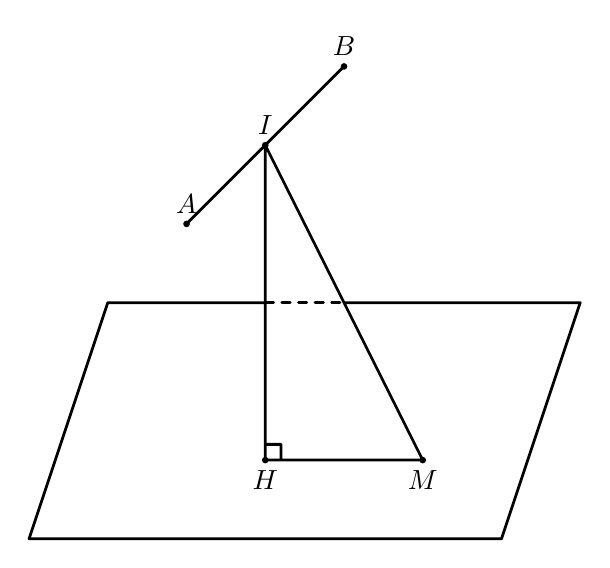
\begin{tikzpicture}[>=stealth,line join=round,line width=1pt, line cap=round]
				\draw (0,1)--(-2,1)--(-3,-2)--(3,-2)--(4,1)--(1,1) (0,-1)--(2,-1)--(0,3)--(0,-1) (-1,2)--(1,4) (0,-0.8)--(0.2,-0.8)--(0.2,-1);
				\draw[dashed] (0,1)--(1,1);
				\fill (-1,2)node[above]{$A$}circle(1.2pt);
				\fill (1,4)node[above]{$B$}circle(1.2pt);
				\fill (0,3)node[above]{$I$}circle(1.2pt);
				\fill (0,-1)node[below]{$H$}circle(1.2pt);
				\fill (2,-1)node[below]{$M$}circle(1.2pt);
		\end{tikzpicture}\end{center}
		Gọi $I$ là điểm thỏa mãn $\overrightarrow{IA}+\overrightarrow{IB}=\overrightarrow{0}$. Suy ra $I$ là trung điểm của $AB$, do đó $I(3;1;4)$.\\  
		Ta có $\overrightarrow{MA}\cdot\overrightarrow{MB}=(\overrightarrow{MI}+\overrightarrow{IA})\cdot(\overrightarrow{MI}+\overrightarrow{IB})=MI^2+\overrightarrow{MI}\cdot(\overrightarrow{IA}+\overrightarrow{IB})=MI^2$.\\
		Gọi $H$ là hình chiếu của $I$ xuống mặt phẳng $(\alpha)$. Khi đó ta có 
		$\overrightarrow{MA}\cdot\overrightarrow{MB}=MI^2\geq IH^2$.\\
		Vậy giá trị nhỏ nhất của $\overrightarrow{MA}\cdot\overrightarrow{MB}$ là $IH^2$, đạt được khi $M\equiv H$.\\
		Đường thẳng đi qua $I$ vuông góc với mặt phẳng $(\alpha)$ là $\Delta\colon \heva{&x=3+t\\&y=1+2t\\&z=4-3t.}$\\
		Do $H$ là hình chiếu vuông góc của $I$ lên $(\alpha)$ nên $H=\Delta\cap (\alpha)$; suy ra $H(4;3;1)$.\\
		\textbf{Cách 2}\\
		Gọi $ M(x;y;z)\in(\alpha)\Rightarrow x+2y-3z-7=0$.\\
		Ta có 	$\overrightarrow{MA}=(4-x;-2-y;6-z)$; $\overrightarrow{MB}=(2-x;4-y;2-z)$.
		\begin{align*} \overrightarrow{MA}\cdot\overrightarrow{MB}=&(4-x)(2-x)+(-2-y)(4-y)+(6-z)(2-z)\\ =&x^2+y^2+z^2-6x-2y-8z+12=(x-3)^2+(y-1)^2+(z-4)^2-12. \end{align*}
		Áp dụng bđt Bunhinacopxki - Cauchy - Schwarz.
		\begin{align*} &\left[1^2+2^2+\left(-3\right)^2\right]\left[\left(x-3\right)^2+\left(y-1\right)^2+\left(z-4\right)^2\right]\geq\left[x-3+2\left(y-1\right)-3\left(z-4\right)\right]^2\\ \Leftrightarrow &14\left[(x-3)^2+(y-1)^2+(z-4)^2\right]\geq{\left[x+2y-3z+7\right]^2}\\ \Leftrightarrow&(x-3)^2+(y-1)^2+(z-4)^2\geq\dfrac{\left(7+7\right)}{14}^2\\ \Leftrightarrow &(x-3)^2+(y-1)^2+(z-4)^2-12\geq 2.\end{align*}
		$ \min\left(\overrightarrow{MA}\cdot\overrightarrow{MB}\right)=2$ xảy ra khi và chỉ khi $$\heva{&x+2y-3z-7=0\\&\dfrac{x-3}{1}=\dfrac{y-1}{2}=\dfrac{z-4}{-3}}\Leftrightarrow\heva{&x=4\\&y=3\\&z=1}\Rightarrow M(4;3;1).$$
	}
\end{ex}

\begin{ex}%[2H2C2-5]
	Trong KG $Oxyz$, cho $A(1;-1;2)$, $B(-2,0,3)$, $C(0;1;-2)$. Gọi $M(a;b;c)$ là điểm thuộc mặt phẳng $(Oxy)$ sao cho biểu thức $S=\overrightarrow{MA}\cdot\overrightarrow{MB}+2\overrightarrow{MB}\cdot\overrightarrow{MC}+3\overrightarrow{MC}\cdot\overrightarrow{MA}$ đạt giá trị nhỏ nhất. Khi đó $ T=12a+12b+c$ có giá trị bằng
	\choice
	{$ T=3$}
	{$ T=-3$}
	{$ T=1$}
	{\True $ T=-1$}
	\loigiai
	{Xét 
		\begin{align*} S=&\overrightarrow{MA}\cdot\overrightarrow{MB}+2\overrightarrow{MB}\cdot\overrightarrow{MC}+3\overrightarrow{MC}\cdot\overrightarrow{MA}\\ =&(\overrightarrow{MI}+\overrightarrow{IA})(\overrightarrow{MI}+\overrightarrow{IB})+2(\overrightarrow{MI}+\overrightarrow{IB})(\overrightarrow{MI}+\overrightarrow{IC})+3(\overrightarrow{MI}+\overrightarrow{IC})(\overrightarrow{MI}+\overrightarrow{IA})\\
			=&6M{I^2}+\overrightarrow{MI}(4\overrightarrow{IA}+3\overrightarrow{IB}+5\overrightarrow{IC})+\overrightarrow{IA}\overrightarrow{IB}+2\overrightarrow{IB}\overrightarrow{IC}+3\overrightarrow{IC}\overrightarrow{IA}.\end{align*}
		Gọi I là điểm thỏa mãn $ 4\overrightarrow{IA}+3\overrightarrow{IB}+5\overrightarrow{IC}=\overrightarrow 0\Rightarrow I\left(\dfrac{-1}{6},\dfrac{1}{12},\dfrac{7}{12}\right)$.\\
		Mà: $\heva{&4\overrightarrow{IA}+3\overrightarrow{IB}+5\overrightarrow{IC}=\overrightarrow{0}\\ &\overrightarrow{IA}\cdot\overrightarrow{IB}+2\overrightarrow{IB}\cdot\overrightarrow{IC}+3\overrightarrow{IC}\cdot\overrightarrow{IA}=\text{const}.}$ \\
		Do đó $S_{\min}\Leftrightarrow MI_{\min}$, điều này xảy ra khi $M$ là hình chiếu của $I$ lên mặt $Oxy$.\\
		Ta dễ dàng tìm được tọa độ $M\left(-\dfrac{1}{6},\dfrac{1}{12},0\right)\Rightarrow T=12a+12b+c=-1$.}
\end{ex}

\begin{ex}%[2H2C2-5]
	Trong không gian với hệ trục tọa độ $Oxyz$, cho các điểm $A(4;1;5)$, $B(3;0;1)$, $C(-1;2;0)$ và điểm $ M(a;b;c)$ thỏa mãn $\overrightarrow{MA}\cdot\overrightarrow{MB}+2\overrightarrow{MB}\cdot\overrightarrow{MC}-5\overrightarrow{MC}\cdot\overrightarrow{MA}$ lớn nhất. Tính $P=a-2b+4c$.
	\choice
	{$P=23$}
	{$P=31$}
	{$P=11$}
	{\True $P=13$}
	\loigiai
	{Đặt  $Q=\overrightarrow{MA}\cdot\overrightarrow{MB}+2\overrightarrow{MB}\cdot\overrightarrow{MC}-5\overrightarrow{MC}\cdot\overrightarrow{MA}$.
		\begin{align*}	&\left(\overrightarrow{MA}-\overrightarrow{MB}\right)^2=MA^2+MB^2-2\overrightarrow{MA}\cdot\overrightarrow{MB}\Rightarrow\overrightarrow{MA}\cdot\overrightarrow{MB}=\dfrac{1}{2}\left(MA^2+MB^2-AB^2\right)\\		&\left(\overrightarrow{MB}-\overrightarrow{MC}\right)^2=MB^2+MC^2-2\overrightarrow{MB}\cdot\overrightarrow{MC}\Rightarrow 2\overrightarrow{MB}\cdot\overrightarrow{MC}=MB^2+MC^2-BC^2\\
			&\left(\overrightarrow{MC}-\overrightarrow{MA}\right)^2=MC^2+MA^2-2\overrightarrow{MC}\cdot\overrightarrow{MA}\Rightarrow\overrightarrow{MC}\cdot\overrightarrow{MA}=\dfrac{1}{2}\left(MC^2+MA^2-AC^2\right).\end{align*}
		Từ đây, ta suy ra 
		\begin{align*} Q=&\overrightarrow{MA}\cdot\overrightarrow{MB}+2\overrightarrow{MB}\cdot\overrightarrow{MC}-5\overrightarrow{MC}\cdot\overrightarrow{MA}\\
			=&\dfrac{1}{2}\left(MA^2+MB^2-AB^2\right)+MB^2+MC^2-BC^2-\dfrac{5}{2}\left(MC^2+MA^2-AC^2\right)\\ =&-2MA^2+\dfrac{3}{2}MB^2-\dfrac{3}{2}MC^2-\dfrac{1}{2}AB^2-BC^2+\dfrac{5}{2}AC^2.\end{align*}
		Gọi $ E$ là điểm thỏa mãn $-2\overrightarrow{EA}+\dfrac{3}{2}\overrightarrow{EB}-\dfrac{3}{2}\overrightarrow{EC}=\overrightarrow{0}\Leftrightarrow\overrightarrow{EA}=\dfrac{3}{4}\overrightarrow{CB}\Leftrightarrow E\left(1;\dfrac{5}{2};\dfrac{17}{4}\right)$.\\
		
		Ta có 
		\begin{align*} Q=&-2MA^2+\dfrac{3}{2}MB^2-\dfrac{3}{2}MC^2-\dfrac{1}{2}AB^2-BC^2+\dfrac{5}{2}AC^2\\
			=&-2\left(\overrightarrow{ME}+\overrightarrow{EA}\right)^2+\dfrac{3}{2}\left(\overrightarrow{ME}+\overrightarrow{EB}\right)^2-\dfrac{3}{2}\left(\overrightarrow{ME}+\overrightarrow{EC}\right)^2-\dfrac{1}{2}AB^2-BC^2+\dfrac{5}{2}AC^2\\
			=&-2ME^2-2EA^2+\dfrac{3}{2}EB^2-\dfrac{3}{2}EC^2-\dfrac{1}{2}AB^2-BC^2+\dfrac{5}{2}AC^2\\
			\leq&-2EA^2+\dfrac{3}{2}EB^2-\dfrac{3}{2}EC^2-\dfrac{1}{2}AB^2-BC^2+\dfrac{5}{2}AC^2.
		\end{align*}
		Vì $T=-2EA^2+\dfrac{3}{2}EB^2-\dfrac{3}{2}EC^2\le-2EA^2+\dfrac{3}{2}EB^2-\dfrac{3}{2}EC^2-\dfrac{1}{2}AB^2-BC^2+\dfrac{5}{2}AC^2=\text{const}$ không đổi nên $Q$ đạt giá trị lớn nhất khi $ME=0\Rightarrow M\equiv E$.\\
		Vậy $M\left(1;\dfrac{5}{2};\dfrac{17}{4}\right)\Rightarrow P=a-2b+4c=13$.}
\end{ex}

\begin{ex} %[2H2C2-5]
	Trong KG $Oxyz$, cho ba điểm $A(-8;1;1)$, $B(2;1;3)$ và $C(6;4;0)$. Một điểm $M$ di động trong không gian sao cho $\overrightarrow{MA}\cdot\overrightarrow{MC}=\overrightarrow{MA}\cdot\overrightarrow{MB}+34$. Biết rằng $\left|MA-MB\right|$ đạt giá trị lớn nhất khi điểm $M$ trùng với điểm $M_0(x_0;y_0;z_0)$. Tích số $x_0y_0z_0$ bằng.
	\choice
	{$16$}
	{\True $18$}
	{$14$}
	{$12$}
	\loigiai{Gọi $M=(a;b;c)$.\\
		Ta có $\overrightarrow{MA}\cdot\overrightarrow{MC}=\overrightarrow{MA}\cdot\overrightarrow{MB}+34\Leftrightarrow\overrightarrow{MA}\left(\overrightarrow{MC}-\overrightarrow{MB}\right)=34\Leftrightarrow\overrightarrow{MA}\cdot\overrightarrow{BC}=34$.\\
		Mặt khác $\overrightarrow{MA}=(-8-a;1-b;1-c)$, $\overrightarrow{BC}=(4;3;-3)$.\\
		Suy ra $4(-8-a)+3(1-b)-3(1-c)=34\Leftrightarrow-4a-3b+3c-66=0$.\\
		Vậy $M\in (P)$ có phương trình $-4x-3y+3z-66=0$.\\
		Ký hiệu $f(M)=f(x;y;z)=-4x-3y+3z-66$, với $M(x;y;z)$.\\
		Ta có $f(A)\cdot f(B)=(-4(-8)-3.1+3.1-66)(-4.2-3.1+3.3-66)=2312>0$.\\
		Suy ra điểm $A(-8;1;1)$ và điểm $B(2;1;3)$ nằm về cùng 1 phía so với mặt phẳng $(P)$.\\
		Khi đó $\left|MA-MB\right|\leq AB$ (tính chất 3 cạnh của tam giác) suy ra $\left|MA-MB\right|$ đạt giá trị lớn nhất khi $M$, $A$, $B$ thẳng hàng và $M$ nằm ngoài đoạn thẳng $AB$ hay $M$ là giao điểm của đường thẳng $AB$ với mặt phẳng $(P)$.\\
		Đường thẳng $AB$ có véc tơ chỉ phương $\overrightarrow{AB}=(10,0,2)$ và qua điểm $B(2,1,3)$ nên có phương trình $\heva{&x=2+5t\\&y=1\\&z=3+t.}$\\
		Suy ra $-4(2+5t)-3+3(3+t)-66=0\Leftrightarrow t=-4$.\\
		Vậy $M(-18,1,-1)$ hay $x_0y_0z_0=18$.
	}
\end{ex}
\Closesolutionfile{ans}
\indapan{6}{ans/ans-C5B3CD5-LC}

\TNSA
\Opensolutionfile{ans}[ans/ans-C5B3CD5-KQ]
\begin{ex} %[2H2C2-5]
	Trong KG $Oxyz$ cho $A(3;2;1)$, $B(-2;3;6)$. Điểm $ M(x_M;y_M;z_M)$ thay đổi thuộc mặt phẳng $(Oxy)$. Tìm giá trị của biểu thức $ T=x_M+y_M+z_M$ khi $\left|\overrightarrow{MA}+3\overrightarrow{MB}\right|$ nhỏ nhất.
	\shortans[]{$2$}
	\loigiai{
		Gọi điểm $H$ thỏa mãn $\overrightarrow{HA}+3\overrightarrow{HB}=\overrightarrow{0}$ khi đó $\heva{&{x_H}=\dfrac{x_A+3x_B}{1+3}\\
			&{y_H}=\dfrac{y_A+3y_B}{1+3}\\
			&{z_H}=\dfrac{z_A+3z_B}{1+3}}\Rightarrow H\left(-\dfrac{3}{4};\dfrac{11}{4};\dfrac{19}{4}\right)$.\\
		Ta có $\left|\overrightarrow{MA}+3\overrightarrow{MB}\right|=4|\overrightarrow{MH}|=4MH$.\\
		Biểu thức $\left|\overrightarrow{MA}+3\overrightarrow{MB}\right|$ đạt giá trị nhỏ nhất khi và chỉ khi $MH$ nhỏ nhất, khi đó $M$ là hình chiếu của $H$ lên mặt phẳng $Oxy$.\\	
		Ta có $H\left(-\dfrac{3}{4};\dfrac{11}{4};\dfrac{19}{4}\right)\Rightarrow M\left(-\dfrac{3}{4};\dfrac{11}{4};0\right)$.\\
		Vậy $T=x_M+y_M+z_M$$=-\dfrac{3}{4}+\dfrac{11}{4}+0=2$.}
\end{ex}

\begin{ex}%[2H2C2-5]
	Trong không gian với hệ trục $Oxyz$, cho các điểm $A(-1;2;3)$, $B(6,-5,8)$ và $\overrightarrow{OM}=a\overrightarrow{i}+b\overrightarrow{k}$, trong đó $a$, $b$ là các số thực luôn thay đổi. Nếu $\left|\overrightarrow{MA}-2\overrightarrow{MB}\right|$ đạt giá trị nhỏ nhất thì giá trị $a-b$ bằng bao nhiêu ?
	\shortans[]{$0$}
	\loigiai{
		Ta có $\overrightarrow{OM}=a\overrightarrow{i}+b\overrightarrow{k}\Rightarrow M(a;0;b)$.\\
		Ta tính được 
		$\heva{&\overrightarrow{MA}=(-1-a;2;3-b)\\&\overrightarrow{MB}=(6-a;-5;8-b)}\Rightarrow \overrightarrow{MA}-2\overrightarrow{MB}=(a-13;12;b-13)$. \\
		Suy ra, $\left|\overrightarrow{MA}-2\overrightarrow{MB}\right|^2=(a-13)^2+144+(b-13)^2\geq 144$, do đó $\min \left|\overrightarrow{MA}-2\overrightarrow{MB}\right|=12$ đạt được khi $\heva{&a=13\\&b=13}$. Vậy $a-b=0$.
	}
\end{ex}

\begin{ex}%[2H2C2-5]
	Trong KG $Oxyz$, cho ba điểm $ A(-1;2;5)$, $B(3;-1;0)$, $C(-4;0;-2)$. Gọi $I$ là điểm trên mặt phẳng $(Oxy)$ sao cho biểu thức $\left|\overrightarrow{IA}-2\overrightarrow{IB}+3\overrightarrow{IC}\right|$ đạt giá trị nhỏ nhất. Tính khoảng cách từ $I$ đến mặt phẳng $(P)\colon 4x+3y+2=0$.
	\shortans[]{$6$}
	\loigiai{
		Gọi $M$ là điểm thỏa $\overrightarrow{MA}-2\overrightarrow{MB}+3\overrightarrow{MC}=\overrightarrow{0}\Rightarrow M\left(-\dfrac{19}{2};2;-\dfrac{1}{2}\right)$.\\
		Ta có: \begin{align*}\left|\overrightarrow{IA}-2\overrightarrow{IB}+3\overrightarrow{IC}\right|=&\left|\overrightarrow{IM}+\overrightarrow{MA}-2\overrightarrow{IM}-2\overrightarrow{MB}+3\overrightarrow{IM}+3\overrightarrow{MC}\right|\\ =&\left|2\overrightarrow{IM}+\left(\overrightarrow{MA}-2\overrightarrow{MB}+3\overrightarrow{MC}\right)\right|=2\left|\overrightarrow{IM}\right|=2IM.
		\end{align*}
		Biểu thức $\left|\overrightarrow{IA}-2\overrightarrow{IB}+3\overrightarrow{IC}\right|$ đạt giá trị nhỏ nhất $\Leftrightarrow IM$ nhỏ nhất, điều này tương đương $ I$ là hình chiếu vuông góc của $ M$ lên $\left(Oxy\right)$. Do đó $I\left(-\dfrac{19}{2};2;0\right)$.\\
		Khoảng cách từ điểm $ I$ đến mặt phẳng $(P)$ là $\mathrm{d}(I;(P))=\dfrac{\left|4\cdot\left(-\dfrac{19}{2}\right)+3\cdot 2+2\right|}{\sqrt{4^2+3^2}}=6$.
	}
\end{ex}
\begin{ex}%[2H2C2-5]
	Trong KG $Oxyz$, cho hai điểm $A(1;2;1)$; $B(2;-1;3)$ và điểm $M(a;b;0)$ sao cho $MA^2+MB^2$ nhỏ nhất. Tính giá trị của $a+b$ bằng 
	\shortans[]{$2$}
	\loigiai{
		Gọi $I$ là trung điểm của $AB$, khi đó $\overrightarrow{IA}+\overrightarrow{IB}=\overrightarrow{0}$ và $I\left(\dfrac{3}{2};\dfrac{1}{2};2\right)$.\\
		Ta có $MA^2+MB^2=2IM^2+IA^2+IB^2=2IM^2+\dfrac{AB^2}{2}=IM^2+7$.\\
		Để $MA^2+MB^2$ nhỏ nhất thì $MI$ nhỏ nhất, mà $M(a;b;0)\in (Oxy)$. Do đó $M$ là hình chiếu vuông góc của $I$ lên $(Oxy)$. Suy ra $M\left(\dfrac{3}{2};\dfrac{1}{2};0\right)$.\\
		Như vậy $a=\dfrac{3}{2},b=\dfrac{1}{2}\Rightarrow a+b=\dfrac{3}{2}+\dfrac{1}{2}=2$ .}
\end{ex}
\begin{ex}%[2H2C2-5]
	Trong không gian cho ba điểm $A(1;1;1)$, $B(-1;2;1)$, $C(3;6;-5)$. Điểm $M(a,b,c)$ thuộc mặt phẳng $(Oxy)$ sao cho $MA^2+MB^2+MC^2$ đạt giá trị nhỏ nhất. Giá trị của $ab$ bằng
	\shortans[]{$3$}
	\loigiai{
		Lấy $ G(1;3;-1)$ là trọng tâm của tam giác $ABC$.\\
		Ta có $MA^2+MB^2+MC^2=3MG^2+GA^2+GB^2+GC^2$.\\
		Do đó $MA^2+MB^2+MC^2$ bé nhất khi $MG$ bé nhất hay $M$ là hình chiếu của điểm $G$ lên mặt phẳng $Oxy$. Vậy $ M(1;3;0)$.}
\end{ex}
\begin{ex}%[2H2C2-5]
	Trong KG $Oxyz$, cho $A(0;1;2)$, $B(1;1;0)$, $C(3;0;1)$ và mặt phẳng $(Q)\colon x+y+z-5=0$. Xét điểm $M$ thay đổi thuộc $(Q)$. Giá trị nhỏ nhất của biểu thức $MA^2+MB^2+MC^2$ bằng $\dfrac{a}{b}$ với $a$, $b$ là hai số tự nhiên nguyên tố cùng nhau. Giá trị $a+b$ bằng
	\shortans[]{$37$}
	\loigiai{
		Gọi điểm $G$ thỏa $\overrightarrow{GA}+\overrightarrow{GB}+\overrightarrow{GC}=\overrightarrow 0$, suy ra $G\left(\dfrac{4}{3};\dfrac{2}{3};1\right)$.\\
		Khi đó $P=MA^2+MB^2+MC^2=3MG^2+GA^2+GB^2+GC^2$\\
		$\Rightarrow P\geq 3\left[\mathrm{d}(G,(Q))\right]^2+GA^2+GB^2+GC^2$.\\
		Dấu bằng xảy ra khi $M$ là hình chiếu của $G$ lên mặt phẳng $(Q)$.\\
		Ta có 
		$\heva{&d\left(G,(Q)\right)=\dfrac{\left|\dfrac{4}{3}+\dfrac{2}{3}+1-5\right|}{\sqrt 3}=\dfrac{2}{\sqrt 3}\\
			&\overrightarrow{GA}=\left(-\dfrac{4}{3};\dfrac{1}{3};1\right)\Rightarrow G{A^2}=\dfrac{26}{9},\\ &\overrightarrow{GB}=\left(-\dfrac{1}{3};\dfrac{1}{3};-1\right)\Rightarrow G{B^2}=\dfrac{11}{9},\\ &\overrightarrow{GC}=\left(\dfrac{5}{3};-\dfrac{2}{3};0\right)\Rightarrow G{C^2}=\dfrac{29}{9}.}$\\
		Vậy $\min P=\dfrac{34}{3}$ khi $M$ là hình chiếu của $G$ lên mặt phẳng $(Q)$.}
\end{ex}
\begin{ex} %[2H2C2-5]
	Trong KG $Oxyz$, cho bốn điểm $A(2;4;-1)$, $B(1;4;-1)$, $C(2;4;3)$ và $D(2;2;-1)$, biểu thức $MA^2+MB^2+MC^2+MD^2$ đạt giá trị nhỏ nhất khi $M(x;y;z)$. Giá trị $x+y+z$ bằng
	\shortans[]{$5{,}25$}
	\loigiai{
		Chọn điểm $I$ sao cho $\overrightarrow{IA}+\overrightarrow{IB}+\overrightarrow{IC}+\overrightarrow{ID}=\overrightarrow{0}$. Khi đó $I\left(\dfrac{7}{4};\dfrac{7}{2};0\right)$.\\
		Ta có $MA^2+MB^2+MC^2+MD^2=4MI^2+IA^2+IB^2+IC^2+ID^2$.\\
		Do $I$, $A$, $B$, $C$, $D$ cố định nên $IA^2+IB^2+IC^2+ID^2$ không đổi.\\
		Do đó để $MA^2+MB^2+MC^2+MD^2$ đạt giá trị nhỏ nhất thì $MI$ nhỏ nhất, tức là $MI=0$, hay $M\equiv I$.\\
		Vậy $I\left(\dfrac{7}{4};\dfrac{7}{2};0\right)$ nên $x+y+z=\dfrac{21}{4}$.
	}
\end{ex}
\begin{ex} %[2H2C2-5]
	Trong KG $Oxyz$, cho ba điểm $A(0;0;1)$, $B(-1;1;0)$, $C(1;0;-1)$. Điểm $M$ di động trên mặt phẳng $(P)\colon 2x+2y-z+2=0$. Biết giá trị nhỏ nhất của $3MA^2+2MB^2+MC^2$ là $\dfrac{a}{b}$ với $a$, $b$ là hai số tự nhiên nguyên tố cùng nhau. Giá trị $a-b$ bằng
	\shortans[]{$55$}
	\loigiai{
		Gọi $I$ là điểm thỏa mãn $3\overrightarrow{IA}+2\overrightarrow{IB}+\overrightarrow{IC}=\overrightarrow{0}\Rightarrow I\left(-\dfrac{1}{6};\dfrac{1}{3};\dfrac{1}{3}\right)$.\\
		Ta có $3MA^2+2MB^2+MC^2=3IA^2+2IB^2+IC^2+6IM^2$.\\
		Do đó $3MA^2+2MB^2+MC^2$ nhỏ nhất khi và chỉ khi $IM$ nhỏ nhất, tương đương $M$ là hình chiếu của $I$ trên $(P)$.\\
		Khi đó $\min IM=\mathrm{d}(I,(P))=\dfrac{2}{3}$, suy ra $\min (3MA^2+2MB^2+MC^2)=\dfrac{61}{6}$.
		%PTĐT đi qua $I$ vuông góc với mặt phẳng $(P)$ là $\Delta\colon \heva{&x=-\dfrac{1}{6}+2t\\&y=\dfrac{1}{3}+2t\\&z=\dfrac{1}{3}-t}$.\\
		%$M$ là hình chiếu của $I$ lên $(P)$ nên $M=\Delta\cap (P)$, suy ra $M\left(-\dfrac{11}{18};-\dfrac{1}{9};\dfrac{5}{9}\right)$
		% $\Rightarrow M\left(-\dfrac{11}{18};-\dfrac{1}{9};\dfrac{5}{9}\right)$ 
	}
\end{ex}

\begin{ex} %[2H2C2-5]
	Trong KG $Oxyz$, cho ba điểm $A(2;-2;4)$, $B(-3;3;-1)$, $C(-1;-1;-1)$ và mặt phẳng $(P)\colon 2x-y+2z+8=0$. Xét điểm $M$ thay đổi thuộc $(P)$, tìm giá trị nhỏ nhất của biểu thức $T=2MA^2+MB^2-MC^2$.
	\shortans[]{$102$}
	\loigiai{
		Gọi $I$ là điểm thỏa $2\overrightarrow{IA}+\overrightarrow{IB}-\overrightarrow{IC}=\overrightarrow{0}\Rightarrow I(1;0;4)$.\\
		Ta có $T=2MA^2+MB^2-MC^2=2MI^2+(2IA^2+IB^2-IC^2)$.\\
		Để $T$ nhỏ nhất thì $ 2MI^2$ nhỏ nhất $\Leftrightarrow MI$ ngắn nhất $M$ là hình chiếu của điểm $I$ lên $(P)$. Khi đó $MI=\mathrm{d}\left(I,(P)\right)=6$ và $2IA^2+IB^2-IC^2=30$, suy ra $\min T=102$.}
\end{ex}

\begin{ex} %[2H2C2-5]
	Trong không gian với hệ trục tọa độ $Oxyz$, cho ba điểm $A(1;4;5)$, $B(3;4;0)$, $C(2;-1;0)$ và mặt phẳng $(\alpha)\colon 3x-3y-2z-12=0$ Gọi $M(a;b;c)$ thuộc $(\alpha)$ sao cho $MA^2+MB^2+3MC^2$ đạt giá trị nhỏ nhất. Tính tổng $S=a+b+c$.
	\shortans[]{$3$}
	\loigiai{
		Gọi $I$ là điểm thỏa $\overrightarrow{IA}+\overrightarrow{IB}+3\overrightarrow{IC}=\overrightarrow{0}\Rightarrow I(2;1;1).$\\
		Mặt khác $MA^2+MB^2+3MC^2=5MI^2+IA^2+IB^2+3IC^2$.\\
		Vì $I$, $A$, $B$, $C$ cố định nên $ IA^2+IB^2+3IC^2$ không đổi.\\
		Do đó $ MA^2+MB^2+3MC^2$ nhỏ nhất $\Leftrightarrow MI^2$ nhỏ nhất $\Leftrightarrow MI$ nhỏ nhất. Điều này xảy ra khi $M$ là hình chiếu của $I$ trên mặt phẳng $(\alpha)$.\\
		PTĐT $\Delta$ qua $I$ và vuông góc với mặt phẳng $(\alpha)$ là $\heva{&x=2+3t\\&y=1-3t\\&z=1-2t.}$\\
		$M$ là hình chiếu của $I$ lên $(\alpha)$ nên $M=\Delta\cap (\alpha)$; suy ra $M\left(\dfrac{7}{2};-\dfrac{1}{2};0\right)$.\\
		Vậy $S=a+b+c=3$.}
\end{ex}

\begin{ex} %[2H2C2-5]
	Trong không gian tọa độ $Oxyz$, cho hai điểm $A(3;-2;2)$, $B(-2;2;0)$ và mặt phẳng $(P)\colon 2x-y+2z-3=0$. Xét các điểm $M$, $N$ di động trên $(P)$ sao cho $MN=1$. Tính giá trị nhỏ nhất của biểu thức $2AM^2+3BN^2$. (kết quả làm tròn đế 1 chữ số thập phân).
	\shortans[]{$49{,}8$}
	\loigiai{
		Gọi $H$, $K$ lần lượt là hình chiếu của $A$, $B$ trên mặt phẳng $(P)$, khi đó ta tìm được $AH=BK=3$, $H(1;-1;0)$, $K(0;1;2)$ nên $HK=3$.\\
		Đặt $HM=t$ ta có $HM+MN+NK\geq HK=3\Rightarrow NK\geq 2-t$\\
		\begin{align*} 2AM^2+3BN^2= &2(AH^2+HM^2)+3(BK^2+KN^2)\\ \geq &45+2t^2+(2-t)^2=\left(\sqrt 3 t-\dfrac{2}{\sqrt 3}\right)^2+\dfrac{143}{3}\ge\dfrac{143}{3}.\end{align*}
		Dấu bằng xảy ra khi $ M$, $N$ thuộc đoạn thẳng $HK$.\\
		Vậy giá trị nhỏ nhất của biểu thức $ 2AM^2+3BN^2$ bằng $\dfrac{143}{3}\approx49{,}8$.}
\end{ex}

\begin{ex} %[2H2C2-5]
	Trong KG $Oxyz$, cho điểm $A(a;b;c)$ với $a$, $b$, $c$ là các số thực dương thỏa mãn $5(a^2+b^2+c^2)=9(ab+2bc+ca)$ và $Q=\dfrac{a}{b^2+c^2}-\dfrac{1}{(a+b+c)^3}$ có giá trị lớn nhất. Gọi $M$, $N$, $P$ lần lượt là hình chiếu vuông góc của $A$ lên các tia $Ox$, $Oy$, $Oz$. Khi đó phương trình mặt phẳng $(MNP)$ là $mx+ny+pz-1=0$. Giá trị $m+np$ bằng
	\shortans[]{$147$}
	\loigiai{
		Đặt $t=b+c$, khi đó $t>0$; $b^2+c^2\geq\dfrac{t^2}{2}$; $bc\leq\dfrac{t^2}{4}$.\\
		\begin{align*} &5(a^2+b^2+c^2)=9(ab+2bc+ca)\\ \Leftrightarrow &5a^2+5\left(b+c\right)^2-9a\left(b+c\right)=28bc\\ \Rightarrow &5a^2+5t^2-9at\leq 7t^2\Leftrightarrow(5a+t)(a-2t)\leq 0\Leftrightarrow a\leq 2t.\end{align*}
		Vậy $Q\leq\dfrac{4}{t}-\dfrac{1}{27t^3}=f(t)$ với $t > 0$.\\
		Ta có  $f'(t)=-\dfrac{4}{t^2}+\dfrac{1}{9t^4}$, $\,\,$ $f'(t)=0\Leftrightarrow t=\dfrac{1}{6}$ (vì $t>0$).\\
		Ta có bảng biến thiên
		\begin{center}
\begin{tikzpicture}[>=stealth]
				\tkzTabInit[nocadre=false,lgt=1.3,espcl=2,deltacl=0.5]{$x$/1.2 ,$f'(t)$/.9,$f(t)$/2}
				{$0$ , $\dfrac{1}{6}$ , $+\infty$}
				\tkzTabLine{ , + , $0$ , - , }
				\tkzTabVar{-/$-\infty$ , +/$16$ , -/$0$}
		\end{tikzpicture}\end{center}
		Vậy $\max Q=16$ đạt được khi $a=\dfrac{1}{3}$; $b=c=\dfrac{1}{12}$.\\
		Suy ra tọa độ điểm $A\left(\dfrac{1}{3};\dfrac{1}{12};\dfrac{1}{12}\right)$; tọa độ các điểm $M\left(\dfrac{1}{3};0;0\right)$; $N\left(0;\dfrac{1}{12};0\right)$; $P\left(0;0;\dfrac{1}{12}\right)$.\\
		Phương trình mặt phẳng $\left(MNP\right)$ $\dfrac{x}{\dfrac{1}{3}}+\dfrac{y}{\dfrac{1}{12}}+\dfrac{z}{\dfrac{1}{12}}=1$ $\Leftrightarrow 3x+12y+12z-1=0$.\\ Suy ra $m+np=147$.}
\end{ex}
\Closesolutionfile{ans}
\indapan{6}{ans/ans-C5B3CD5-KQ}
\begin{dang}{Giá trị lớn nhất, giá trị nhỏ nhất liên quan đến khoảng cách}
\end{dang}
\noindent{\bf Bài toán 1. Trong không gian hệ tọa độ $Oxyz$, cho điểm $A\left(x_0;y_0;z_0\right)$ cố định và điểm $M$ di động trên mặt phẳng $(P)\colon Ax+By+Cz+D=0$. Tìm tọa độ điểm $M$ để $AM$ có giá trị nhỏ nhất}\\
{\bf Phương pháp giải}\\
{\bf Cách 1. Phương pháp hình học}
\begin{itemize}
	\item Bước 1:
	\begin{center}
		\begin{tikzpicture}[scale=1, font=\footnotesize, line join=round, line cap=round, >=stealth]
			\coordinate (O) at (0,0);
			\coordinate (B) at (0.6,2);
			\coordinate (C) at (6,2);
			\coordinate (D) at ($(O)+(C)-(B)$);
			\coordinate (H) at (4,1);
			\coordinate (A) at ($(H)+(0,2)$);\coordinate (M) at ($(H)-(2,0)$);
			\coordinate (F) at (intersection of B--C and A--H);
			\coordinate (E) at (intersection of B--C and A--M);
			\draw (O)--(B)--(E) (F)--(C)--(D)--(O) (M)--(A)--(H)--(M);
			\draw[dashed] (F)--(E);
			\draw pic[draw]{angle = D--O--B} node[above right=-0.1]{$P$};
			\pic[draw,angle radius=2mm] {right angle = A--H--M};
			\foreach \i/\g in {M/-90,A/90,H/-90}{\draw[fill=black](\i) circle (1.5pt) ($(\i)+(\g:3mm)$) node[scale=1]{$\i$};}
		\end{tikzpicture}
	\end{center}
	+ Gọi $H$ là hình chiếu vuông góc của $A$ trên mặt phẳng $(P)$.\\
	+ Khi đó, tam giác $AHM$ vuông tại $H$, suy ra $AM\ge AH$. \\
	+ Đẳng thức xảy ra khi $M\equiv H$. \\
	+ Do đó $AM$ nhỏ nhất khi $M$ là hình chiếu của $A$ trên mặt phẳng $(P)$.
	\item Bước 2: Tìm tọa độ điểm $M$ ($M\equiv H$).\\
	+ Lập PTTS đường thẳng $AH$ với $\heva{
		& \text{ đi qua điểm }A \\ 
		&\overrightarrow{u}_{AH}=\overrightarrow{n}_P=(a;b;c).}$\\
	+ Ta có $M\equiv H=AH\cap (P)\Rightarrow $ tọa độ điểm $M$ cần tìm. 
\end{itemize}
{\bf Cách 2. Phương pháp đại số}\\
Dùng bất đẳng thức bộ $3$ của Bunhiacốpxki.\\
Với $a$, $b$, $c$, $x$, $y$, $z\in \mathbb{R}$, ta có
$$(ax+by+cz)^2\le (a^2+b^2+c^2)(x^2+y^2+z^2).$$
Dấu bằng xảy ra $\Leftrightarrow \dfrac{a}{x}=\dfrac{b}{y}=\dfrac{c}{z}$.\\
\noindent{\bf Bài toán $2$. Trong KG $Oxyz$, cho hai điểm $A$, $B$ cố định. Lập phương trình mặt phẳng $(P)$ đi qua $A$ và cách $B$ một khoảng lớn nhất.}\\
{\bf Phương pháp giải}\\
{\bf Cách 1: Phương pháp hình học}
\begin{center}
	\begin{tikzpicture}[scale=1, font=\footnotesize, line join=round, line cap=round, >=stealth]
		\coordinate (O) at (0,0);
		\coordinate (I) at (1,2);
		\coordinate (J) at (6,2);
		\coordinate (Q) at ($(O)+(J)-(I)$);
		\coordinate (H) at (4,1);
		\coordinate (B) at ($(H)+(0,2)$);\coordinate (A) at ($(H)-(2,0)$);
		\coordinate (F) at (intersection of I--J and B--H);
		\coordinate (E) at (intersection of I--J and B--A);
		\draw (O)--(I)--(E) (F)--(J)--(Q)--(O) (A)--(B)--(H);
		\draw[dashed] (F)--(E);
		\draw pic[draw]{angle = Q--O--I} node[above right=-0.1]{$P$};
		\pic[draw,angle radius=2mm] {right angle = A--H--B};
		\foreach \i/\g in {B/90,A/-90,H/-90}{\draw[fill=black](\i) circle (1pt) ($(\i)+(\g:3mm)$) node[scale=1]{$\i$};}
	\end{tikzpicture}
\end{center}
\begin{itemize}
	\item Bước 1:\\
	+ Gọi $H$ là hình chiếu của $B$ lên mặt phẳng $(P)$.\\
	+ Khi đó $\mathrm{d}(B,(P))=BH\le BA$.\\
	+ Do đó $(P)$ là mặt phẳng đi qua $A$ vuông góc với $AB$.
	\item Bước 2: Lập phương trình mặt phẳng $(P)$ với $\heva{
		& \text{đi qua điểm } A \\ 
		& \overrightarrow{n}_P=\overrightarrow{AB}.}$
\end{itemize}
{\bf Cách 2: Phương pháp đại số}
\begin{itemize}
	\item Gọi $\overrightarrow{n}_P=(a;b;c)$, $(a^2+b^2+c^2\ne 0 $ là một véc-tơ pháp tuyến của mặt phẳng $(P)$. 
	\item Khi đó phương trình mặt phẳng $(P)$ đi qua điểm $A$ là
	$$a(x-x_A)+b(y-y_A)+c(z-z_A)=0.$$
	\item Khi đó $\overrightarrow{n}_P\cdot \overrightarrow{AB}=0$ từ đây ta rút được theo $a$ theo $b$, $c$ (hoặc $b$ theo $a$, $c$ hoặc $c$ theo $a$, $b$).
	\item Ta có $\mathrm{d}(B;(P))=f(t)$, với $t=\dfrac{b}{c}$, $c\neq 0$.\\
	+ Khảo sát $f(t)$ ta tìm được max của $f(t)$.
	\begin{note}
		Để tìm véc-tơ pháp tuyến $\overrightarrow{n}_P$ của $(P)$ đơn giản hơn thì nên gọi $\overrightarrow{n}_P=(1;b;c)$.
	\end{note}
\end{itemize}
{\bf Bài toán 3. Trong không gian hệ tọa độ $Oxyz$, cho điểm $A$ và đường thẳng $\Delta $ cố định. Lập phương trình mặt phẳng $(P)$ đi qua đường thẳng $\Delta $ và cách $A$ một khoảng lớn nhất.}\\
{\bf Phương pháp giải}\\
{\bf Cách 1: Phương pháp hình học}

\begin{itemize}
	\item Bước 1
	\begin{center}
		\begin{tikzpicture}[scale=1, font=\footnotesize, line join=round, line cap=round, >=stealth]
			\coordinate (O) at (0,0);
			\coordinate (B) at (0.6,2);
			\coordinate (C) at (6,2);
			\coordinate (D) at ($(O)+(C)-(B)$);
			\coordinate (H) at (2,1);\coordinate (K) at (4,1);
			\coordinate (A) at ($(H)+(0,2)$);
			\coordinate (T) at ($(C)!5/3!(K)$);\coordinate (U) at ($(K)!1/3!(C)$);
			\coordinate (E) at (intersection of B--C and A--H);
			\coordinate (F) at (intersection of B--C and A--K);
			\draw (O)--(B)--(E) (F)--(C)--(D)--(O) (M)--(A)--(H) (A)--(K) (T)--(U);
			\draw[dashed] (F)--(E);
			\draw pic[draw]{angle = D--O--B} node[above right=-0.1]{$P$};
			\pic[draw,angle radius=2mm] {right angle = A--H--K};
			\pic[draw,angle radius=2mm] {right angle = A--K--U};
			\foreach \i/\g in {K/-90,A/90,H/-90}{\draw[fill=black](\i) circle (1.5pt) ($(\i)+(\g:3mm)$) node[scale=1]{$\i$};}
			\draw (U) node[above]{$\Delta$};
		\end{tikzpicture}
	\end{center}
	+ Gọi $H$, $K$ lần lượt là hình chiếu của $A$ lên mặt phẳng $(P)$ và đường thẳng $\Delta$.\\   
	+ Khi đó $\mathrm{d}(A,(P))=AH\le AK$.\\
	+ Do đó $(P)$ là mặt phẳng đi qua $K$ và vuông góc với $AK$. 
	\item Bước 2.\\
	+ Tìm tọa độ điểm $K$.\\
	+ Lập phương trình mặt phẳng $(P)$ với $\heva{
		& \text{đi qua điểm } K \\ 
		& \overrightarrow{n}_P=\overrightarrow{AK}.}$
\end{itemize}
{\bf Cách 2: Phương pháp đại số}\\
+ Gọi $\overrightarrow{n}_P=(a;b;c)$, $(a^2+b^2+c^2\ne 0)$ là một véc-tơ pháp tuyến của mặt phẳng $(P)$.\\
+ Khi đó $\overrightarrow{n}_P\cdot \overrightarrow{u}_{\Delta }=0$ từ đây ta rút được $a$ theo $b$, $c$ (hoặc $b$ theo $a, c$ hoặc $c$ theo $a, b$).\\
+ Ta có $\mathrm{d}(A,(P))=f(t)$, với $t=\dfrac{b}{c}$, $c\neq 0$.\\ 
+ Khảo sát $f(t)$ ta tìm được max của $f(t)$.
\begin{note}
	Để tìm véc-tơ pháp tuyến $\overrightarrow{n}_P$ của $(P)$ đơn giản hơn thì nên gọi $\overrightarrow{n}_P=(1;b;c)$.
\end{note}
{\bf Bài toán 4. Trong không gian hệ tọa độ $Oxyz$, cho mặt phẳng $(P)$ và hai điểm phân biệt $A$, $B$. Tìm điểm $M$ thuộc $(P)$ sao cho 
	\begin{enumEX}{2}
		\item $MA+MB$ nhỏ nhất.
		\item $|MA-MB|$ lớn nhất.
	\end{enumEX}
}
{\bf Phương pháp giải}
\begin{enumEX}{1}
	\item $MA+MB$ nhỏ nhất.\\
	Ta xét hai trường hợp sau:
	\begin{itemize}
		\item TH1: Nếu $A$ và $B$ nằm về hai phía so với $(P)$. 
		Khi đó $AM+BM\ge AB$.\\
		Đẳng thức xảy ra khi $M$ là giao điểm của $AB$ với $(P)$.
		\item TH2: Nếu $A$ và $B$ nằm cùng một phía so với $(P)$.\\
		Gọi $A'$ đối xứng với $A$ qua $(P)$.\\
		Khi đó $AM+BM=A'M+BM\ge A'B$.\\
		Đẳng thức xảy ra khi $M$ là giao điểm của $A'B$ với $(P)$.
		\begin{center}
			\begin{tikzpicture}[scale=1, font=\footnotesize, line join=round, line cap=round, >=stealth]
				\coordinate (O) at (0,0);
				\coordinate (P) at (0.6,2);
				\coordinate (Q) at (6,2);
				\coordinate (R) at ($(O)+(Q)-(P)$);
				\coordinate (H) at (2,1);\coordinate (M) at (4,1);
				\coordinate (A) at ($(H)+(-1,2)$);
				\coordinate (B) at ($(A)!2!(H)$);
				\coordinate (U) at (intersection of A--B and O--R);
				\coordinate (V) at (intersection of M--B and O--R);
				\coordinate (E) at (intersection of P--Q and A--H);
				\coordinate (F) at (intersection of P--Q and A--M);
				\draw (O)--(P) (Q)--(R)--(O) (H)--(A)--(M) (V)--(B)--(U) (P)--(E) (F)--(Q);
				\draw[dashed] (H)--(U) (M)--(V) (E)--(F);
				\draw pic[draw]{angle = R--O--P} node[above right=-0.1]{$P$};
				\draw[fill=black] (H) circle (1.5pt);
				\foreach \i/\g in {B/-90,A/90,M/0}{\draw[fill=black](\i) circle (1.5pt) ($(\i)+(\g:3mm)$) node[scale=1]{$\i$};}
			\end{tikzpicture}
			\begin{tikzpicture}[scale=1, font=\footnotesize, line join=round, line cap=round, >=stealth]
				\coordinate (O) at (0,0);
				\coordinate (P) at (0.6,2);
				\coordinate (Q) at (6,2);
				\coordinate (R) at ($(O)+(Q)-(P)$);
				\coordinate (H) at (2,1);\coordinate (M) at (3,1.5);
				\coordinate (K) at (4,1);
				\coordinate (A) at ($(H)+(0,2)$);
				\coordinate (A') at ($(A)!2!(H)$);
				\coordinate (B) at ($(A')!1.8!(K)$);
				\coordinate (U) at (intersection of A--A' and O--R);
				\coordinate (V) at (intersection of A'--B and O--R);
				\coordinate (E) at (intersection of P--Q and A--H);
				\coordinate (F) at (intersection of P--Q and A--M);
				\coordinate (I) at (intersection of P--Q and B--M);
				\coordinate (J) at (intersection of P--Q and A'--B);
				\draw (O)--(P) (Q)--(R)--(O) (H)--(A)--(M)--(B)--(K) (V)--(A')--(U) (P)--(E) (F)--(I) (J)--(Q);
				\draw[dashed] (H)--(U) (K)--(V) (M)--(A') (E)--(F) (I)--(J);
				\draw pic[draw]{angle = R--O--P} node[above right=-0.1]{$P$};
				\pic[draw,angle radius=2mm] {right angle = A--H--M};
				\draw[fill=black] (H) circle (1.5pt);
				\foreach \i/\g in {B/90,A/90,M/180,A'/-90,H/180}{\draw[fill=black](\i) circle (1.5pt) ($(\i)+(\g:3mm)$) node[scale=1]{$\i$};}
			\end{tikzpicture}
		\end{center}
	\end{itemize}
	\item $|MA-MB|$ lớn nhất.\\
	Ta xét hai trường hợp sau:
	\begin{itemize}
		\item TH1: Nếu $A$ và $B$ nằm cùng một phía so với $(P)$.\\
		+ Khi đó $|AM-BM|\le AB$.\\
		+ Đẳng thức xảy ra khi $M$ là giao điểm của $AB$ với $(P)$.
		\item TH2: Nếu $A$ và $B$ nằm khác phía so với $(P)$.\\
		+ Gọi $A'$ đối xứng với $A$ qua $(P)$. \\
		+ Khi đó $|AM-BM|=|A'M-BM|\le AB$.\\
		+ Đẳng thức xảy ra khi $M$ là giao điểm của $A'B$ với $(P)$.
	\end{itemize}
\end{enumEX}
{\bf Bài toán 5. Trong không gian hệ tọa độ $Oxyz$, cho các số thực dương $\alpha$, $\beta$ và ba điểm $A$, $B$, $C$. Viết phương trình mặt phẳng $(P)$ đi qua $C$ và thỏa mãn $T=\alpha \mathrm{d}(A,(P))+\beta \mathrm{d}(B,(P))$  nhỏ nhất.}\\
{\bf Phương pháp giải}
\begin{itemize}
	\item TH1. Xét  $A$, $B$ nằm về cùng phía so với $(P)$.\\
	+ Nếu $AB\parallel (P)$ thì $P=\left(\alpha+\beta\right)\mathrm{d}(A,(P))\le \left(\alpha+\beta\right)AC$.\\
	+ Nếu đường thẳng $AB$ cắt $(P)$ tại $I$. Gọi $D$ là điểm thỏa mãn $\overrightarrow{IB}=\dfrac{\alpha}{\beta}\overrightarrow{ID}$ và $E$ là trung điểm $BD$.\\
	Khi đó $P=\alpha \mathrm{d}(A;(P))+\beta\cdot \dfrac{IB}{ID}\cdot \mathrm{d}(D,(P))=2\alpha \mathrm{d}(E,(P))=2\left(\alpha+\beta\right)EC$.
	\item TH2. Xét $A$, $B$ nằm về hai phía so với $(P)$.\\
	Gọi $I$ là giao điểm của $AB$ và $(P)$, $B'$ là điểm đối xứng với $B$ qua $I$.\\ 
	Khi đó $P=\alpha \mathrm{d}(A,(P))+\beta \mathrm{d}(B',(P))$.\\
	Đến đây ta chuyển về {\bf Bài toán 4} trên.
\end{itemize}
{\bf Bài toán 6. Trong không gian hệ tọa độ $Oxyz$, cho $n$ điểm $A_1$, $A_2$,\ldots, $A_n$ và điểm $A$. Viết phương trình mặt phẳng $(P)$ đi qua $A$ và tổng khoảng cách từ các điểm $A_i$ ($i=\overline{1,n}$) lớn nhất.}\\
{\bf Phương pháp giải}
\begin{itemize}
	\item Xét $n$ điểm $A_1$, $A_2$,\ldots, $A_n$ nằm cùng phía so với $(P)$. Gọi $G$ là trọng tâm của $n$ điểm đã cho.\\ 
	Khi đó $\sum\limits_{i=1}^{n}\mathrm{d}(A_i,(P))=n\mathrm{d}(G,(P))\le n GA$.
	\item Trong $n$ điểm trên có $m$ điểm nằm về một phía và $k$ điểm nằm về phía khác ($m+k=n$). Khi đó, gọi $G_1$ là trọng tâm của $m$ điểm, $G_2$ là trọng tâm của  điểm $G_3$ đối xứng với $G_1$ qua $A$.\\
	Khi dó $P=m \mathrm{d}(G_3,(P))+k\mathrm{d}(G_2,(P))$.
\end{itemize}
Đến đây ta chuyển về {\bf Bài toán 5} trên.
\Opensolutionfile{ans}[ans/ans-C5B3CD5]
\TN
%Câu 37
\begin{ex}%[2H5V1-5] 
	Trong không gian hệ tọa độ $Oxyz$, cho điểm $A(1;2;-2)$. Gọi $(P)$ là mặt phẳng chứa trục $Ox$ sao cho khoảng cách từ $A$ đến $(P)$ lớn nhất. Phương trình của $(P)$ là
	\choice
	{$2y+z=0$}
	{$2y-z=0$ }
	{$y+z=0$}
	{\True $y-z=0$}
	\loigiai{
		\begin{center}
			\begin{tikzpicture}[scale=1, font=\footnotesize, line join=round, line cap=round, >=stealth]
				\coordinate (O) at (0,0);
				\coordinate (B) at (0.6,2);
				\coordinate (C) at (6,2);
				\coordinate (D) at ($(O)+(C)-(B)$);
				\coordinate (H) at (2,1);\coordinate (K) at (4,1);
				\coordinate (A) at ($(H)+(0,2)$);
				\coordinate (T) at ($(C)!5/3!(K)$);\coordinate (U) at ($(K)!1/3!(C)$);
				\coordinate (E) at (intersection of B--C and A--H);
				\coordinate (F) at (intersection of B--C and A--K);
				\draw (O)--(B)--(E) (F)--(C)--(D)--(O) (A)--(H) (A)--(K) (T)--(U);
				\draw[dashed] (F)--(E);
				\draw pic[draw]{angle = D--O--B} node[above right=-0.1]{$P$};
				\pic[draw,angle radius=2mm] {right angle = A--H--K};
				\foreach \i/\g in {K/-90,A/90,H/-90}{\draw[fill=black](\i) circle (1.5pt) ($(\i)+(\g:3mm)$) node[scale=1]{$\i$};}
				\draw (U) node[right]{$Ox$};
			\end{tikzpicture}
		\end{center}
		Gọi $K$ là hình chiếu vuông góc của $A(1;2;-2)$ trên $Ox$, suy ra $K(1;0;0),$
		$\overrightarrow{AK}=(0;-2;2)$.\\
		Gọi $H$ là điểm chiếu của $A$ lên mặt phẳng $(P)$.
		Ta có $\mathrm{d}(A,(P))=AH\le AK=2\sqrt{2}$.\\
		Suy ra $\mathrm{d}(A,(P))=2\sqrt{2}$, đạt được khi $H\equiv K(1;0;0)$.\\
		Khi đó mặt phẳng $(P)$ qua $O(0;0;0)$ có một véc-tơ pháp tuyến là $\overrightarrow{AK}=(0;-2;2)$.\\
		Phương trình mặt phẳng $(P)$ là $0(x-1)-2(y-0)+2(z-0)=0\Leftrightarrow y-z=0$.\\
		Vậy $(P)\colon y-z=0$.
} \end{ex} 
%Câu 38
\begin{ex}%[2H5V1-5]
	Trong không gian hệ trục tọa độ $Oxyz$, mặt phẳng $(P)$ đi qua điểm $A(1;7;2)$ và cách $M(-2;4;-1)$ một khoảng lớn nhất có phương trình là
	\choice
	{$(P)\colon 3x+3y+3z-10=0$}
	{$(P)\colon x+y+z-1=0$}
	{\True $(P)\colon x+y+z-10=0$}
	{$(P)\colon x+y+z+10=0$}
	\loigiai{
		Ta có $\mathrm{d}(M,(P))\le MA$.\\
		Khi đó $\mathrm{d}(M,(P))$ lớn nhất là bằng $MA$ khi $A$ là hình chiếu của $M$ trên mặt phẳng $(P)$.\\
		Suy ra $AM\perp (P)\Rightarrow \overrightarrow{AM}=(-3;-3;-3)$ là véc-tơ pháp tuyến của $(P)$.\\
		Mặt phẳng $(P)$ đi qua $A(1;7;2)$ và nhận $\overrightarrow{AM}=(-3;-3;-3)$ là véc-tơ pháp tuyến nên có phương trình $-3(x-1)-3(y-7)-3(z-2)=0\Leftrightarrow x+y+z-10=0$.	
	}
\end{ex}
%Câu 39
\begin{ex}%[2H5V1-5]
	Trong KG $Oxyz$, cho điểm $A(2;-1;-2)$ và đường thẳng $d$ có phương trình $\dfrac{x-1}{1}=\dfrac{y-1}{-1}=\dfrac{z-1}{1}$. Gọi $(P)$ là mặt phẳng đi qua điểm $A$, song song với đường thẳng $d$ và khoảng cách từ $d$ tới mặt phẳng $(P)$ là lớn nhất. Khi đó mặt phẳng $(P)$ vuông góc với mặt phẳng nào sau đây?
	\choice
	{$x-y-6=0$}
	{$x+3y+2z+10$}
	{$x-2y-3z-1=0$}
	{\True $3x+z+2=0$}
	\loigiai{
		\begin{center}
			\begin{tikzpicture}[scale=1, font=\footnotesize, line join=round, line cap=round, >=stealth]
				\coordinate (O) at (0,0);
				\coordinate (B) at (0.6,2);
				\coordinate (C) at (6,2);
				\coordinate (D) at ($(O)+(C)-(B)$);
				\coordinate (A) at (1,1);\coordinate (K) at (3,1);
				\coordinate (H) at ($(K)+(0,2)$);
				\coordinate (T) at ($(H)+(-2,0)$);\coordinate (U) at ($(T)!2!(H)$);
				\coordinate (E) at (intersection of B--C and A--H);
				\coordinate (F) at (intersection of B--C and H--K);
				\draw (O)--(B)--(E) (F)--(C)--(D)--(O) (A)--(H) (A)--(K) (T)--(U) (H)--(K);
				\draw[dashed] (F)--(E);
				\draw pic[draw]{angle = D--O--B} node[above right=-0.1]{$P$};
				\pic[draw,angle radius=2mm] {right angle = A--H--T};
				\foreach \i/\g in {K/-90,A/180,H/90}{\draw[fill=black](\i) circle (1.5pt) ($(\i)+(\g:3mm)$) node[scale=1]{$\i$};}
				\draw (U) node[right]{$d$};
			\end{tikzpicture}
		\end{center}
		Gọi $H$ là hình chiếu của $A$ lên đường thẳng $d$, suy ra $H(1;1;1)$.\\
		Gọi $(P)$ là mặt phẳng đi qua điểm $A$ và $(P)$ song song với đường thẳng $d$.\\
		Gọi $K$ là hình chiếu của $H$ lên mặt phẳng $(P)$.\\
		Do $d\parallel (P)$ nên ta có $\mathrm{d}(d,(P))=\mathrm{d}(H,(P))=HK$.\\
		Ta luôn có bất đẳng thức $HK\le HA$.\\
		Như vậy khoảng cách từ $d$ đến $(P)$ lớn nhất bằng $AH$.\\
		Và khi đó $(P)$ nhận $\overrightarrow{AH}=(-1;2;3)$ làm véc-tơ pháp tuyến.\\
		Do $(P)$ đi qua $A(2;-1;-2)$ nên ta có phương trình của $(P)$ là $x-2y-3z-10=0$.\\
		Do đó $(P)$ vuông góc với mặt phẳng có phương trình $3x+z+2=0$.
	}
\end{ex}
%Câu 40
\begin{ex}%[2H5V1-5]
	Trong không gian với hệ toạ độ $Oxyz$, gọi $(P)$ là mặt phẳng đi qua hai điểm $A(1;-7;-8)$, $B(2;-5;-9)$ sao cho khoảng cách từ điểm $M(7;-1;-2)$ đến $(P)$ đạt giá trị lớn nhất. Biết $(P)$ có một véc-tơ pháp tuyến là $\overrightarrow{n}=(a;b;4)$, khi đó giá trị của tổng $a+b$ là
	\choice
	{$-1$}
	{\True $3$}
	{$6$}
	{$2$}
	\loigiai{
		\begin{center}
			\begin{tikzpicture}[scale=1, font=\footnotesize, line join=round, line cap=round, >=stealth]
				\coordinate (O) at (0,0);
				\coordinate (B) at (0.6,2);
				\coordinate (C) at (6,2);
				\coordinate (D) at ($(O)+(C)-(B)$);
				\coordinate (H) at (2,1);\coordinate (K) at (4,1);
				\coordinate (M) at ($(H)+(0,2)$);
				\coordinate (T) at ($(C)!5/3!(K)$);\coordinate (U) at ($(K)!1/3!(C)$);
				\coordinate (E) at (intersection of B--C and M--H);
				\coordinate (F) at (intersection of B--C and M--K);
				\draw (O)--(B)--(E) (F)--(C)--(D)--(O) (M)--(H) (M)--(K) (T)--(U);
				\draw[dashed] (F)--(E);
				\draw pic[draw]{angle = D--O--B} node[above right=-0.1]{$P$};
				\pic[draw,angle radius=2mm] {right angle = M--H--K};
				\pic[draw,angle radius=2mm] {right angle = M--K--U};
				\foreach \i/\g in {K/-90,M/90,H/-90}{\draw[fill=black](\i) circle (1.5pt) ($(\i)+(\g:3mm)$) node[scale=1]{$\i$};}
				\draw (U) node[right]{$AB$};
			\end{tikzpicture}
		\end{center}
		PTTS của đường thẳng $AB$ là $\heva{&x=1+t\\&y=-7+2t\\&z=-8-t.}$\\
		Gọi $H$, $K$ lần lượt là hình chiếu của $M$ trên $(P)$ và đường thẳng $AB$.\\
		Vì $K\in AB$ nên $K(1+t;-7+2t;-8-t)\Rightarrow \vec{MK}=(6-t;6-2t;6+t)$.\\
		Đường thẳng $AB$ có véc-tơ chỉ phưng là $\vec{u}=(1;2;-1)$.\\
		Ta có $\vec{MK}\cdot \vec{u}=0\Leftrightarrow 6-t+2(6-2t)-(6+t)=0\Leftrightarrow t=2$.\\
		Ta tìm được điểm $K(3;-3;-10)$.\\
		Ta luôn có bất đẳng thức $\mathrm{d}(M;(P))=MH\le AK$.\\
		Dấu bằng xảy ra khi và chỉ khi $H\equiv K$. Khi đó $\overrightarrow{MH}=(-4;-2;-8)=-2(2;1;4)$.\\
		Mặt phẳng $(P)$ có một véc-tơ pháp tuyến là $\overrightarrow{n}=(2;1;4)$.\\
		Vậy ta có $a+b=3$.
	}
\end{ex}
%Câu 41
\begin{ex}%[2H5V1-5]
	Trong KG $Oxyz$, cho điểm $A(3;-1;0)$ và đường thẳng $d\colon \dfrac{x-2}{-1}=\dfrac{y+1}{2}=\dfrac{z-1}{1}$. Mặt phẳng $(\alpha)$ chứa $d$ sao cho khoảng cách từ $A$ đến $(\alpha)$ lớn nhất có phương trình là
	\choice
	{$x+y-z-2=0$}
	{\True $x+y-z=0$}
	{$x+y-z+1=0$}
	{$-x+2y+z+5=0$}
	\loigiai{
		\begin{center}
			\begin{tikzpicture}[scale=1, font=\footnotesize, line join=round, line cap=round, >=stealth]
				\coordinate (O) at (0,0);
				\coordinate (B) at (0.6,2);
				\coordinate (C) at (6,2);
				\coordinate (D) at ($(O)+(C)-(B)$);
				\coordinate (H) at (2,1);\coordinate (K) at (4,1);
				\coordinate (A) at ($(H)+(0,2)$);
				\coordinate (T) at ($(C)!5/3!(K)$);\coordinate (U) at ($(K)!1/3!(C)$);
				\coordinate (E) at (intersection of B--C and A--H);
				\coordinate (F) at (intersection of B--C and A--K);
				\draw (O)--(B)--(E) (F)--(C)--(D)--(O) (A)--(H) (A)--(K) (T)--(U);
				\draw[dashed] (F)--(E);
				\draw pic[draw]{angle = D--O--B} node[above right=-0.1]{$P$};
				\pic[draw,angle radius=2mm] {right angle = A--H--K};
				\pic[draw,angle radius=2mm] {right angle = A--K--U};
				\foreach \i/\g in {K/-90,A/90,H/-90}{\draw[fill=black](\i) circle (1.5pt) ($(\i)+(\g:3mm)$) node[scale=1]{$\i$};}
				\draw (U) node[right]{$d$};
			\end{tikzpicture}
		\end{center}
		Gọi $H$, $K$ lần lượt là hình chiếu của $A$ lên $(\alpha)$ và $d$, suy ra $AH\le AK$.\\
		Vì $H\in d$ nên $H(2-t;-1+2t;1+t)\Rightarrow \overrightarrow{AH}=(-1-t;2t;1+t)$.\\
		Do $AH\perp d$ nên ta có $-(-1-t)+2\cdot 2t+1+t=0\Leftrightarrow t=-\dfrac{1}{3}$.\\
		Khi đó $\overrightarrow{AH}=\left(-\dfrac{2}{3};-\dfrac{2}{3};\dfrac{2}{3}\right)$.\\
		Khoảng cách từ $A$ đến $(\alpha)$ lớn nhất khi và chỉ khi $AH=AK$.\\
		Do đó $(\alpha)$ có véc-tơ pháp tuyến là $\overrightarrow{n}=(1;1;-1)$.\\
		Vậy $(\alpha)\colon 1\cdot (x-2)+1\cdot (y+1)-1\cdot (z-1)=0\Leftrightarrow x+y-z=0$.
		\begin{note}
			Vẫn là đánh giá bất đẳng thức $AH\le AK$ nói trên, nhưng bài toán sau đây lại phát biểu hơi khác một chút.
		\end{note}
	}
\end{ex}
%Câu 42
\begin{ex}%[2H5V1-5]
	Trong không gian hệ tọa độ $Oxyz$, cho đường thẳng $d\colon \dfrac{x+1}{-2}=\dfrac{y}{1}=\dfrac{z-1}{1}$ và điểm $A(1;2;3)$. Gọi $(P)$ là mặt phẳng chứa $d$ và cách điểm $A$ một khoảng cách lớn nhất. Véc-tơ nào dưới đây là một véc-tơ pháp tuyến của $(P)$.
	\choice
	{$\overrightarrow{n}=(1;0;2)$}
	{$\overrightarrow{n}=(1;0;-2)$}
	{\True $\overrightarrow{n}=(1;1;1)$}
	{$\overrightarrow{n}=(1;1;-1)$}
	\loigiai{
		\begin{center}
			\begin{tikzpicture}[scale=1, font=\footnotesize, line join=round, line cap=round, >=stealth]
				\coordinate (O) at (0,0);
				\coordinate (B) at (0.6,2);
				\coordinate (C) at (6,2);
				\coordinate (D) at ($(O)+(C)-(B)$);
				\coordinate (K) at (2,1);\coordinate (H) at (4,1);
				\coordinate (A) at ($(K)+(0,2)$);
				\coordinate (T) at ($(C)!5/3!(H)$);\coordinate (U) at ($(H)!1/3!(C)$);
				\coordinate (E) at (intersection of B--C and A--H);
				\coordinate (F) at (intersection of B--C and A--K);
				\draw (O)--(B)--(E) (F)--(C)--(D)--(O) (A)--(H) (A)--(K) (T)--(U);
				\draw[dashed] (F)--(E);
				\draw pic[draw]{angle = D--O--B} node[above right=-0.1]{$P$};
				\pic[draw,angle radius=2mm] {right angle = A--H--U};
				\pic[draw,angle radius=2mm] {right angle = A--K--H};
				\foreach \i/\g in {K/-90,A/90,H/-90}{\draw[fill=black](\i) circle (1.5pt) ($(\i)+(\g:3mm)$) node[scale=1]{$\i$};}
				\draw (U) node[right]{$d$};
			\end{tikzpicture}
		\end{center}
		Gọi $H$ là hình chiếu vuông góc của $A$ lên đường thẳng $d$, gọi $K$ là hình chiếu vuông góc của $A$ lên $(P)$.\\
		Do đó khoảng cách từ $A$ đến $(P)$ là $\mathrm{d}(A;(P))=AK$.\\
		Ta có $d\colon \heva{&x=-1-2t\\&y=t\\&z=1+t}$. Vì $H\in d$ nên $H(-2t-1;t;t+1)$.\\
		Suy ra $\overrightarrow{AH}=(-2t-2;t-2;t-2)$, véc-tơ chỉ phương của đường thẳng $d$ là $\overrightarrow{u}_d=(-2;1;1)$.\\
		Ta có $\overrightarrow{AH}\cdot \overrightarrow{u}_d=0\Leftrightarrow -2(-2t-2)+t-2+t-2=0\Leftrightarrow t=0$.\\
		Do đó $H(-1;0;1)$ và $\overrightarrow{AH}=(-2;-2;-2)\Rightarrow AH=2\sqrt{3}$ (không đổi).\\
		Vì $AK\le AH$ (đường vuông góc luôn ngắn hơn đường xiên) nên $AK$ lớn nhất khi $AK=AH$ hay $K\equiv H$.\\
		Suy ra $\overrightarrow{AK}=\overrightarrow{AH}=(-2;-2;-2)=-2(1;1;1)$.\\
		Vậy một véc-tơ pháp tuyến của $(P)$ là $\overrightarrow{n}=(1;1;1)$.
	}
\end{ex}
%Câu 43
\begin{ex}%[2H5V1-5]
	Trong không gian hệ tọa độ $Oxyz$, cho điểm $A(2;1;3)$ và mặt phẳng $(P)$ có phương trình $x+my+(2m+1)z-m-2=0$, $m$ là tham số. Gọi $H(a;b;c)$ là hình chiếu vuông góc của điểm $A$ trên $(P)$. Tính $a+b$ khi khoảng cách từ điểm $A$ đến  $(P)$ lớn nhất?
	\choice
	{$a+b=-\dfrac{1}{2}$}
	{$a+b=2$}
	{$a+b=0$}
	{\True $a+b=\dfrac{3}{2}$}
	\loigiai{
		Ta có $x+my+(2m+1)z-m-2=0\Leftrightarrow m(y+2z-1)+x+z-2=0\, (*)$.\\
		Phương trình $(*) $ có nghiệm với $\forall m\Leftrightarrow \heva{&y+2z-1=0\\&x+z-2=0.}$\\
		Suy ra $(P)$ luôn đi qua đường thẳng $d\colon \heva{&x=2-t\\&y=1-2t\\&z=t.}$
		\begin{center}
			\begin{tikzpicture}[scale=1, font=\footnotesize, line join=round, line cap=round, >=stealth]
				\coordinate (O) at (0,0);
				\coordinate (B) at (0.6,2);
				\coordinate (C) at (6,2);
				\coordinate (D) at ($(O)+(C)-(B)$);
				\coordinate (H) at (2,1);\coordinate (K) at (4,1);
				\coordinate (A) at ($(H)+(0,2)$);
				\coordinate (T) at ($(C)!5/3!(K)$);\coordinate (U) at ($(K)!1/3!(C)$);
				\coordinate (E) at (intersection of B--C and A--H);
				\coordinate (F) at (intersection of B--C and A--K);
				\draw (O)--(B)--(E) (F)--(C)--(D)--(O) (A)--(H) (A)--(K) (T)--(U);
				\draw[dashed] (F)--(E);
				\draw pic[draw]{angle = D--O--B} node[above right=-0.1]{$P$};
				\pic[draw,angle radius=2mm] {right angle = A--H--K};
				\pic[draw,angle radius=2mm] {right angle = A--K--U};
				\foreach \i/\g in {K/-90,A/90,H/-90}{\draw[fill=black](\i) circle (1.5pt) ($(\i)+(\g:3mm)$) node[scale=1]{$\i$};}
				\draw (V) node[above]{$d$};
				\draw[->] (K)--(U) node[right]{$\overrightarrow{u}$};
			\end{tikzpicture}
		\end{center}
		Gọi $K$ là hình chiếu vuông góc của $A$ trên $d$.\\
		Vì $K\in d\Rightarrow K(2-t;1-2t;t)\Rightarrow \overrightarrow{AK}=(-t;-2t;t-3)$.\\
		Đường thẳng $d$ có véc-tơ chỉ phương $\overrightarrow{u}=(-1;-2;1)$.\\
		Ta có $\overrightarrow{AK}\cdot \overrightarrow{u}=0\Leftrightarrow t+4t+t-3=0\Leftrightarrow t=\dfrac{1}{2}\Rightarrow K\left(\dfrac{3}{2};0;\dfrac{1}{2}\right)$.\\
		Ta có $AH\le AK\Rightarrow AH$ lớn nhất khi $AH=AK$ khi $ H\equiv K$.\\
		Vậy $a+b=\dfrac{3}{2}$.
	}
\end{ex}
%Câu 44
\begin{ex}%[2H5V1-5]
	Trong KG $Oxyz$, cho điểm $A(2;5;3)$ và đường thẳng $d\colon \dfrac{x-1}{2}=\dfrac{y}{1}=\dfrac{z-2}{2}$. Biết rằng $(P)\colon ax+by+cz-3=0$ ($a$, $b$, $c\in \mathbb{Z}$) là mặt phẳng chứa $d$ và khoảng cách từ $A$ đến $(P)$ lớn nhất. Khi đó tổng $T=a+b+c$ bằng
	\choice
	{$3$}
	{$-3$}
	{\True $-2$}
	{$-5$}
	\loigiai{
		\begin{center}
			\begin{tikzpicture}[scale=1, font=\footnotesize, line join=round, line cap=round, >=stealth]
				\coordinate (O) at (0,0);
				\coordinate (B) at (0.6,2);
				\coordinate (C) at (6,2);
				\coordinate (D) at ($(O)+(C)-(B)$);
				\coordinate (H) at (2,1);\coordinate (K) at (4,1);
				\coordinate (A) at ($(H)+(0,2)$);
				\coordinate (T) at ($(C)!5/3!(K)$);\coordinate (U) at ($(K)!1/3!(C)$);
				\coordinate (E) at (intersection of B--C and A--H);
				\coordinate (F) at (intersection of B--C and A--K);
				\draw (O)--(B)--(E) (F)--(C)--(D)--(O) (A)--(H) (A)--(K) (T)--(U);
				\draw[dashed] (F)--(E);
				\draw pic[draw]{angle = D--O--B} node[above right=-0.1]{$P$};
				\pic[draw,angle radius=2mm] {right angle = A--H--K};
				\foreach \i/\g in {K/-90,A/90,H/-90}{\draw[fill=black](\i) circle (1.5pt) ($(\i)+(\g:3mm)$) node[scale=1]{$\i$};}
				\draw (V) node[above]{$d$};
				\draw[->] (K)--(U) node[right]{$\overrightarrow{u}$};
			\end{tikzpicture}
		\end{center}
		Đường thẳng $d$ đi qua $M(1;0;2)$, có một véc-tơ chỉ phương $\overrightarrow{u}=(2;1;2)$.\\
		Gọi $H$, $K$ lần lượt là hình chiếu của $A$ trên $(P)$ và trên $d$ thì $AH\le AK$ (cố định).\\
		Do đó, khoảng cách từ $A$ đến $(P)$ lớn nhất khi $H\equiv K$ hay $(P)\perp AK$.\\
		Gọi $K(2t+1;t;2t+2)\in d$ là hình chiếu của $A$ trên $d$, suy ra $\overrightarrow{AK}=(2t-1;t-5;2t-1)$.\\
		Ta có $\overrightarrow{AK}\cdot \overrightarrow{u}=0\Leftrightarrow 2(2t-1)+(t-5)+2(2t-1)=0\Leftrightarrow t=1$.\\
		Khi đó $(P)$ đi qua $M(1;0;2)$, có một véc-tơ pháp tuyến $\overrightarrow{AK}=(1;-4;1)$ nên $$(P)\colon x-4y+z-3=0.$$
		Vậy $T=a+b+c=1+(-4)+1=-2$.
	}
\end{ex}
%Câu 45
\begin{ex}%[2H5V1-5]
	Trong không gian hệ tọa độ $Oxyz$, cho đường thẳng $d\colon \dfrac{x+1}{-2}=\dfrac{y}{1}=\dfrac{z-1}{1}$ và điểm $A(1;2;3)$. Gọi $(P)$ là mặt phẳng chứa $d$ và cách điểm $A$ một khoảng cách lớn nhất. Véc-tơ nào dưới đây là một véc-tơ pháp tuyến của $(P)$?
	\choice
	{$\overrightarrow{n}=(1;0;2)$}
	{$\overrightarrow{n}=(1;0;-2)$}
	{\True $\overrightarrow{n}=(1;1;1)$}
	{$\overrightarrow{n}=(1;1;-1)$}
	\loigiai{
		\begin{center}
			\begin{tikzpicture}[scale=1, font=\footnotesize, line join=round, line cap=round, >=stealth]
				\coordinate (O) at (0,0);
				\coordinate (B) at (0.6,2);
				\coordinate (C) at (6,2);
				\coordinate (D) at ($(O)+(C)-(B)$);
				\coordinate (H) at (2,1);\coordinate (M) at (4,1);
				\coordinate (A) at ($(H)+(0,2)$);
				\coordinate (T) at ($(C)!5/3!(M)$);\coordinate (U) at ($(M)!1/3!(C)$);
				\coordinate (E) at (intersection of B--C and A--H);
				\coordinate (F) at (intersection of B--C and A--M);
				\draw (O)--(B)--(E) (F)--(C)--(D)--(O) (A)--(H) (A)--(M) (T)--(U) (H)--(M);
				\draw[dashed] (F)--(E);
				\draw pic[draw]{angle = D--O--B} node[above right=-0.1]{$P$};
				\pic[draw,angle radius=2mm] {right angle = A--H--K};
				\foreach \i/\g in {M/-90,A/90,H/-90}{\draw[fill=black](\i) circle (1.5pt) ($(\i)+(\g:3mm)$) node[scale=1]{$\i$};}
				\draw (U) node[right]{$d$};
			\end{tikzpicture}
		\end{center}
		Gọi $H$ là hình chiếu của $A$ xuống mặt phẳng $(P)$.\\
		Từ $H$ kẻ $HM\perp d$. Dễ thấy $AM\perp d$.\\
		Ta có $AH\le AM$. Suy ra khoảng cách từ $A$ đến $(P)$ lớn nhất khi $M\equiv H$, hay $IM\perp (P)$.\\
		PTTS của $d\colon \heva{&x=-1-2t\\&y=t\\&z=1+t} (t\in \mathbb{R})$, véc-tơ chỉ phương là $\overrightarrow{u}=(-2;1;1)$.\\
		Vì $M\in d$ nên $M(-1-2t;t;1+t)\Rightarrow \overrightarrow{MA}=(2-2t;2-t;2-t)$.\\
		Ta có $\overrightarrow{MA}\perp \overrightarrow{u}\Leftrightarrow \overrightarrow{MA}\cdot \overrightarrow{u}=0\Leftrightarrow (-2)\cdot (2+2t)+1\cdot (2-t)+1\cdot (2-t)=0\Leftrightarrow t=0$.\\
		Suy ra $M(-1;0;1)\Rightarrow \overrightarrow{MA}=(2;2;2)$.\\
		Do $\overrightarrow{n}=(1;1;1)$ cùng hướng với $\overrightarrow{MA}$ nên $\overrightarrow{n}=(1;1;1)$ là một véc-tơ pháp tuyến của $(P)$. 
	}
\end{ex}
%Câu 46
\begin{ex}%[2H5V1-5]
	Trong không gian với hệ trục tọa độ $Oxyz$, cho hai điểm $A(1;2;3)$, $B(5;-4;-1)$ và mặt phẳng $(P)$ qua $Ox$ sao cho $\mathrm{d}(B,(P))=2\mathrm{d}(A,(P))$ cắt $AB$ tại $I(a;b;c)$ nằm giữa $AB$. Tính $a+b+c$.
	\choice
	{$8$}
	{$6$}
	{$12$}
	{\True $4$}
	\loigiai{
		Vì mặt phẳng $(P)$ qua $Ox$ nên phương trình mặt phẳng $(P)$ có dạng $by+cz=0$  trong đó $b^2+c^2>0$. Ta có 
		\begin{eqnarray*}
			&&\mathrm{d}(B,(P))=2\mathrm{d}(A,(P))\\
			&\Leftrightarrow& \dfrac{|-4b-c|}{\sqrt{b^2+c^2}}=2\cdot \dfrac{|2b+3c|}{\sqrt{b^2+c^2}}\\
			&\Leftrightarrow&\hoac{&-4b-c=4b+6c\\&-4b-c=-4b-6c}\\
			&\Leftrightarrow&\hoac{&8b+7c=0\\&c=0.}
		\end{eqnarray*}
		\begin{itemize}
			\item TH1. $8b+7c=0$. Chọn $b=7\Rightarrow c=-8\Rightarrow (P)\colon 7y-8z=0$.\\
			Xét $f(x,y,z)=7y-8z$.\\
			Thay tọa độ $A$, $B$ vào ta được $\left(7\cdot 2-8\cdot 3\right)\cdot \left[7\cdot (-4)-8\cdot (-1)\right]>0$.\\
			Suy ra $A$, $B$ nằm cùng phía so với $(P)$ (loại).
			\item TH2. $c=0$, chọn $b=1\Rightarrow (P)\colon y=0$.\\
			Xét $f(x,y,z)=y$. Thay tọa độ $A$, $B$ vào ta được $2\cdot (-4)<0$.\\
			Suy ra $A$, $B$ nằm khác phía so với $(P)$.\\
			Do đó đường thẳng $AB$ cắt $(P)$ tại $I$ nằm giữa $AB$.\\
			PTTS của đường thẳng $AB\colon \heva{&x=1+4t\\&y=2-6t\\&z=3-4t} (t\in \mathbb{R}).$\\
			Tọa độ điểm $I$ là nghiệm hệ phương trình $\heva{&x=1+4t\\&y=2-6t\\&z=3-4t\\&y=0}\Leftrightarrow \heva{&t=\dfrac{1}{3}\\&x=\dfrac{7}{3}\\&y=0\\&z=\dfrac{5}{3}}\Rightarrow I\left(\dfrac{7}{3};0;\dfrac{5}{3}\right)$.\\
			Vậy $a+b+c=\dfrac{7}{3}+0+\dfrac{5}{3}=4$.
		\end{itemize}
	}
\end{ex}
%%%==============EX_1============%%%
\begin{ex}%[2H5V1-5] 
	Trong không gian với hệ trục tọa độ $Oxyz$, cho hai điểm $A(1;2;3)$, $B(5;-4;-1)$ và mặt phẳng $(P)$ qua $Ox$ sao cho $\mathrm{d}(B,(P))=2\mathrm{d}(A,(P))$ cắt $AB$ tại $I(a;b;c)$ nằm giữa $AB$. Tính $a+b+c$.
	\choice
	{$8$}
	{$6$}
	{$12$}
	{\True $4$}
	\loigiai{
		Mặt phẳng $(P)$ qua $Ox$ nên phương trình mặt phẳng $(P)$ có dạng $by+c=0$ $(b^2+c^2>0)$.\\
		Ta có
		\begin{eqnarray*}
			&&\mathrm{d}(B,(P)) =2\mathrm{d}(A,(P))\\
			&\Leftrightarrow&\dfrac{|-4-c|}{\sqrt{b^2+c^2}} =2\cdot \dfrac{2b+3c}{\sqrt{b^2+c^2}}\\
			& \Leftrightarrow &\hoac{&-4b-4b=4b+6c\\&-4b-4b=-4b-6c}\\
			&\Leftrightarrow &\hoac{&8b+7c=0\\ &c=0.}
		\end{eqnarray*}
		\begin{itemize}
			\item Trường hợp 1: $8b+7c=0$.\\
			Chọn $b=7$, $c=-8$, khi đó $(P)\colon7y-8z=0$.\\
			Xét $f(x;y)=7y-8z$, thay tọa độ $A$, $B$ vào ta được $(7\cdot 2-8\cdot 3)(7\cdot (-4)-8\cdot (-1))>0$.\\
			Suy ra $A$, $B$ nằm cùng phía so với $(P)$ (loại).
			\item Trường hợp 2: $c=0$, suy ra phương trình $(P):y=0$.\\
			Thay tọa độ $A$, $B$ vào ta được $2 \cdot (-4) <0$.\\
			Suy ra $A$, $B$ nằm khác phía so với $(P)$. Do đó đường thẳng $AB$ cắt $(P)$ tại $I$ nằm giữa $AB$.\\
			PTTS của đường thẳng $AB\colon \heva{&x=1+4t\\ &y=2-6t\\ &z=3-4t} (t\in \mathbb{R})$.
		\end{itemize}
		Tọa độ điểm $I$ là nghiệm hệ phương trình
		$$\heva{&x=1+4t\\ &y=2-6t\\ &z=3-4t\\ &y=0} \Leftrightarrow \heva{&t=\dfrac{1}{3}\\ &x=\dfrac{7}{3}\\ & y=0\\ &z=\dfrac{5}{3}} \Rightarrow I\left( \dfrac{7}{3};0;\dfrac{5}{3} \right).$$
		Vậy $a+b+c=4$.
	}
\end{ex}

%%%==============EX_2============%%%
\begin{ex}%[2H5V2-5] 
	Trong KG $Oxyz$, cho $A(2;3;-1)$, $B(2;3;2)$, $C(-1;0;2)$.Tìm tọa độ điểm $M$ thuộc mặt phẳng $(Oxz)$ để $S=\left|\overrightarrow{MA}-4\overrightarrow{MC}\right|+\left|\overrightarrow{MA}+\overrightarrow{MB}+\overrightarrow{MC}\right|$ nhỏ nhất.
	\choice
	{\True $M\left(-1;0;\dfrac{7}{3} \right)$}
	{$M(0;3;0)$}
	{$M\left(1;0;\dfrac{7}{3} \right)$}
	{$M\left(-\dfrac{1}{2};0;2\right)$}
	\loigiai{
		Gọi $G$ là trọng tâm tam giác $ABC$, suy ra $G(1;2;1)$.\\
		Gọi $H(x;y;z)$ là điểm thỏa mãn $\overrightarrow{HA}-4\overrightarrow{HC}=\overrightarrow0$.
		$$\Leftrightarrow\heva{&{2-x=4(-1-x)} \\
			&{3-y=4(0-y)} \\
			&{-1-z=4(2-z)}
		} \Leftrightarrow \heva{&{x=-2} \\
			&{y=-1} \\
			&{z=3}
			&} \Rightarrow H(-2;-1;3).$$
		Nhận thấy $G$, $H$ nằm về hai phía đối với mặt phẳng $(Oxz)$ và $HG=\sqrt{22}$.\\
		Ta có
		\begin{eqnarray*}
			&S&=\left|\overrightarrow{MA}-4\overrightarrow{MC}\right|+\left|\overrightarrow{MA}+\overrightarrow{MB}+\overrightarrow{MC}\right|\\
			&&=\left|\overrightarrow{MH}+\overrightarrow{HA}-4\overrightarrow{MH}-4\overrightarrow{HC}\right|+\left|\overrightarrow{MG}+\overrightarrow{GA}+\overrightarrow{MG}+\overrightarrow{GB}+\overrightarrow{MG}+\overrightarrow{GC}\right|\\
			&& =\left|-3\overrightarrow{MH}\right|+\left|3\overrightarrow{MG}\right|\\
			&&=3(MH+MG)\ge 3GH=3\sqrt{22}.
		\end{eqnarray*}
		Đẳng thức xảy ra khi và chỉ khi $H$, $M$, $G$ thẳng hàng theo thứ tự.\\
		Lại do $M\in (Oxz)$ nên $S$ đạt giá trị nhỏ nhất khi và chỉ khi $M$ là giao điểm của đường thẳng $GH$ với mặt phẳng $(Oxz)$.\\
		Đường thẳng $GH$ có phương trình $\heva{&{x=1+3t} \\
			&{y=2+3t} \\
			&{z=1-2t}.}$\\
		Mặt phẳng $(Oxz)$ có phương trình $y=0$.\\
		Ta có $M\in GH\Rightarrow M(1+3t;2+3t;1-2t).$\\		
		Mặt khác $M\in (Oxz)\Rightarrow 2+3t=0\Leftrightarrow t=-\dfrac{2}{3}$.\\
		Vậy $M\left(-1;0;\dfrac{7}{3} \right)$.
	}
\end{ex}

%%%==============EX_3============%%%
\begin{ex}%[2H5C1-3] 
	Trong KG $Oxyz$ cho mặt phẳng $(P)$ đi qua điểm $M(9;1;1)$ cắt các tia $Ox$, $Oy$, $Oz$ lần lượt tại $A$, $B$, $C$ ($A$, $B$, $C$ không trùng với gốc tọa độ). Thể tích tứ diện $OABC$ đạt giá trị nhỏ nhất là bao nhiêu?
	\choice
	{\True $\dfrac{81}{2}$}
	{$\dfrac{243}{2}$}
	{$\dfrac{81}{6}$}
	{$243$}
	\loigiai{
		Giả sử $A(a;0;0)$, $B(0;b;0)$, $C(0;0;c)$ với $a$, $b$, $c$ $>0$.\\
		Mặt phẳng $(P)$ có phương trình đoạn chắn là $\dfrac{x}{a}+\dfrac{y}{b}+\dfrac{z}{c}=1$.\\
		Vì mặt phẳng $(P)$ đi qua điểm $M(9;1;1)$ nên $\dfrac{9}{a}+\dfrac{1}{b}+\dfrac{1}{c}=1$.\\
		Ta có $1=\dfrac{9}{a}+\dfrac{1}{b}+\dfrac{1}{c} \ge 3\sqrt[{3}]{\dfrac{9}{a\cdot b\cdot c}}
		\Rightarrow a\cdot b\cdot c\ge 243$.\\ 
		Khi đó $V_{OABC}=\dfrac{1}{6} a\cdot b\cdot c\ge \dfrac{243}{6}=\dfrac{81}{2}$.\\
		Vậy thể tích tứ diện $OABC$ đạt giá trị nhỏ nhất là $\dfrac{81}{2}$.
	}
\end{ex}

%%%==============EX_4============%%%
\begin{ex}%[2H5C1-5] 
	Trong KG $Oxyz$, cho các điểm $M(m; 0; 0)$, $N(0; n; 0)$, $P(0; 0; p)$ không trùng với gốc tọa độ và thỏa mãn $m^2+n^2+p^2=3$. Tìm giá trị lớn nhất của khoảng cách từ $O$ đến mặt phẳng $(MNP)$.
	\choice
	{$\dfrac{\sqrt{3}}{9}$}
	{$\dfrac{1}{3}$}
	{\True $\dfrac{\sqrt{3}}{3}$}
	{$\dfrac{1}{27}$}
	\loigiai{
		Mặt phẳng $(MNP)$ có phương trình là $\dfrac{x}{m}+\dfrac{y}{n}+\dfrac{z}{p}=1$.\\
		Theo bất đẳng thức Bunhia-Copsky ta có $$\left(m^2+n^2+p^2 \right) \left(\dfrac{1}{m^2}+\dfrac{1}{n^2}+\dfrac{1}{p^2} \right)\ge 9\Rightarrow \dfrac{1}{m^2}+\dfrac{1}{n^2}+\dfrac{1}{p^2} \ge \dfrac{9}{m^2+n^2+p^2}=3.$$
		Khi đó $\mathrm{d}\left(O;(P)\right)=\dfrac{1}{\sqrt{\dfrac{1}{m^2}+\dfrac{1}{n^2}+\dfrac{1}{p^2}}} \le \dfrac{\sqrt{3}}{3}$.\\
		Dấu bằng xảy ra khi $m=n=p=1$.\\
		Vậy khoảng cách lớn nhất từ $O$ đến $(MNP)$ bằng $ \dfrac{\sqrt{3}}{3}$.}
\end{ex}
\Closesolutionfile{ans}
\indapan{10}{ans/ans-C5B3CD5}
%%%==============EX_5============%%%
\TNSA
\Opensolutionfile{ans}[ans/ans-C5B3CD5-KQ]
\begin{ex}%[2H5V1-3]
	Trong KG $Oxyz$, cho điểm $A(2;1;-1)$. Gọi $(P)\colon  ax+by+cz=0$ là mặt phẳng chứa trục $Oy$ sao cho khoảng cách từ $A$ đến $(P)$ là lớn nhất. Tính $a+b+c$.
	\shortans{$1$}
	\loigiai{
		\immini{
			Gọi $H$ là hình chiếu vuông góc của điểm $A$ lên mặt phẳng $(P)$, $A'$ là hình chiếu vuông góc của điểm $A$ lên trục $Oy$. Suy ra $A'(0;1;0)$.\\
			Khi đó $\mathrm{d}\left(A;(P)\right)=AH \le AA'$.\\
			Độ dài đoạn thẳng $AH$ dài nhất khi $H$ và $A'$ trùng nhau. Khi đó mặt phẳng $(P)$ nhận $\overrightarrow{A'A}=(2;0;-1)$ làm véc-tơ pháp tuyến.\\
			Phương trình mặt phẳng $(P)$ đi qua $A'(0;1;0)$ có véc-tơ pháp tuyến $\overrightarrow{A'A}=(2;0;-1)$ là 
			$$2(x-0)+0(y-1)+(-1)(z-0)=0\Leftrightarrow 2x-z=0.$$
			Vậy $a+b+c=1$.	
		}{
			\begin{tikzpicture}[line join=round, line cap=round,>=stealth,thick,scale=0.5]
				%Khai báo điểm----------------------
				\path (0,0) coordinate (H);
				\path (0,3) coordinate (A);
				\path (3,-1) coordinate (A');
				\path (-1,1) coordinate (D);	
				\path (-3,-3) coordinate (E);
				\path (5,-3) coordinate (F);	
				\path (5,0) coordinate (I);
				\path (1,-2) coordinate (G);
				\path pic[draw,angle radius=5pt]{right angle= A--A'--I};
				\path pic[draw,angle radius=5pt]{right angle= A--H--A'};
				\path pic["\scriptsize$P$", angle eccentricity=0.6,draw,angle radius=20pt]{angle= F--E--D};
				%vẽ---------------------------------
				\draw (A)--(H)--(A')--cycle;
				\draw (D)--(E)--(F);
				\draw (I)--(A')--(G);
				\node at (4,0){$Oy$};
				%hiển thị tên điểm----------------------
				\foreach \t/\g in {H/-90,A'/-90,A/90}{
					\draw[fill=black] (\t) circle (1pt) node[shift={(\g:10pt)}]{$ \t $};
				}
			\end{tikzpicture}	
		}
	}
\end{ex}

%%%==============EX_6============%%%
\begin{ex}%[2H5V1-3]
	Trong KG $Oxyz$, cho điểm $A(2;1;1)$. Gọi $(P)\colon ax+by+c=0$ là mặt phẳng chứa trục $Oy$ sao cho khoảng cách từ $A$ đến $(P)$ lớn nhất. Tính $a+b+c$.
	\SA{3}
	\loigiai{
		\immini{
			Gọi $H$ và $K$ lần lượt là hình chiếu của $A$ trên $(P)$ và trục $Oy$.\\
			Ta có $\mathrm{d}\left(A,(P)\right)=AH\le AK$.\\
			Do đó khoảng cách từ $A$ đến $(P)$ lớn nhất khi $H\equiv K(0;1;0)$.\\
			Phương trình $(P)$ đi qua $K(0;1;0)$ và có véc-tơ pháp tuyến $\overrightarrow{AK}=(-2;0;-1)$ là
			$$-2(x-0)+0(y-1)-1(z-0)=0 \Leftrightarrow 2x+z=0.$$
			Vậy $a+b+c=3$.	
		}{
			\begin{tikzpicture}[line join=round, line cap=round,>=stealth,thick,scale=0.5]
				%Khai báo điểm----------------------
				\path (0,0) coordinate (H);
				\path (0,3) coordinate (A);
				\path (3,-1) coordinate (K);
				\path (-1,1) coordinate (D);	
				\path (-3,-3) coordinate (E);
				\path (5,-3) coordinate (F);	
				\path (5,0) coordinate (I);
				\path (1,-2) coordinate (G);
				\path pic[draw,angle radius=5pt]{right angle= A--K--I};
				\path pic[draw,angle radius=5pt]{right angle= A--H--K};
				\path pic["\scriptsize$P$", angle eccentricity=0.6,draw,angle radius=20pt]{angle= F--E--D};
				%vẽ---------------------------------
				\draw (A)--(H)--(K)--cycle;
				\draw (D)--(E)--(F);
				\draw (I)--(K)--(G);
				\node at (4,0){$Oy$};
				%hiển thị tên điểm----------------------
				\foreach \t/\g in {H/-90,K/-90,A/90}{
					\draw[fill=black] (\t) circle (1pt) node[shift={(\g:10pt)}]{$ \t $};
				}
			\end{tikzpicture}	
		}
	}
\end{ex}


%%%==============EX_7============%%%
\begin{ex}%[2H5V1-5]
	Trong KG $Oxyz$, cho điểm $A(1;2;2)$. Gọi $(P)$ là mặt phẳng chứa trục $Ox$ sao cho khoảng cách từ $A$ đến $(P)$ lớn nhất. Phương trình của mặt phẳng $(P)$ có dạng $y+az=0$. Tính $a$.
	\shortans[0]{$1$}
	\loigiai{
		Gọi hình chiếu vuông góc của điểm $A(1;2;2)$ lên trục $Ox$ là $M(1;0;0)$. \\
		Khoảng cách từ $A$ đến $(P)$ lớn nhất nên mặt phẳng $(P)$ có véctơ pháp tuyến là $\overrightarrow{MA}=(0;2;2)$. \\
		Phương trình mặt phẳng $(P)$ đi qua điểm $M(1;0;0)$ và có véctơ pháp tuyến là $\overrightarrow{MA}=(0;2;2)$ có dạng $0.(x-1)+2(y-0)+2(z-0)=0$ $\Leftrightarrow y+z=0$.
	}
\end{ex}
%%%==============EX_8============%%%
\begin{ex}%[2H5V2-7]
	Trong KG $Oxyz$, cho điểm $A(2;-1;-2)$ và đường thẳng $(d)$ có phương trình $\dfrac{x-1}{1}=\dfrac{y-1}{-1}=\dfrac{z-1}{1}$. Gọi $(P)$ là mặt phẳng đi qua điểm $A$, song song với đường thẳng $(d)$ và khoảng cách từ $(d)$ tới mặt phẳng $(P)$ là lớn nhất. Khi đó mặt phẳng $(P)$ có dạng $x+ay+bz+c=0$. Tính $T=a+b+c+d$.
	\shortans[0]{$-15$}
	\loigiai{
		Gọi $H$ là hình chiếu của $A$ lên đường thẳng $d$. Ta suy ra $H(1;1;1)$. \\
		Gọi $(P)$ là mặt phẳng đi qua điểm $A$ và song song với đường thẳng $(d)$. \\
		Gọi $K$ là hình chiếu của $H$ lên mặt phẳng $(P)$. \\
		Do $d\parallel (P)$ nên ta có $\mathrm{d}\left(d,(P)\right)=\mathrm{d}\left(H,(P)\right)=HK \le HA$. \\
		Như vậy khoảng cách từ đến lớn nhất bằng $HA$. Và khi đó $(P)$ nhận $AH=(-1;2;3)$ làm vectơ pháp tuyến. \\
		Do $(P)$ đi qua $A(2;-1;-2)$ nên ta có phương trình của $(P)$ là $x-2y-3z-10=$ nên $T=a+b+c=-15$.
	}
\end{ex}
%%%%==============EX_9============%%%
\begin{ex}%[2H5C1-5]
	Trong KG $Oxyz$, cho điểm $A(2;5;3)$ và đường thẳng $d\colon \dfrac{x-1}{2}=\dfrac{y}{1}=\dfrac{z-2}{2}$. Gọi $(P)$ là mặt phẳng chứa $(d)$ sao cho khoảng cách từ $A$ đến $(P)$ là lớn nhất. Biết khoảng cách từ gốc tọa độ $O$ đến mặt phẳng $(P)$ bằng $\dfrac{m\sqrt{n}}{n}$ với $m,n\in\mathbb{Z}$. Tính $T=m+n$.
	\shortans[0]{$3$}
	\loigiai{
		Gọi $\overrightarrow{n}=(a,b,c)$ là một vectơ pháp tuyến của $(P)$ với $a^2+b^2+c^2\neq 0$. \\
		Điểm $M(1;0;2)\in d \Rightarrow M\in(P)$. \\
		Phương trình của $(P)\colon ax+by+cz-(a+2c)=0$. \\
		Một vectơ chỉ phương của $(d)$ là\\ $\overrightarrow{u}=(2;1;2)\\ \Rightarrow \overrightarrow{n}\perp \overrightarrow{u} \Leftrightarrow \vec{n}\cdot \vec{u}=0 \Leftrightarrow 2a+b+2c=0 \Leftrightarrow b=-2a-2c$.\\
		Khi đó
		$\mathrm{d}\left(A,(P)\right)=\dfrac{|a+5b+c|}{\sqrt{a^2+b^2+c^2}}=\dfrac{9|a+c|}{\sqrt{a^2+c^2+4(a+c)^2}}$. \\
		Ta có $\dfrac{(a+c)^2}{2} \le a^2+c^2$.\\
		Suy ra $a^2+c^2+4(a+c)^2 \ge \dfrac{(a+c)^2}{2} +4(a+c)^2=\dfrac{9}{2}(a+c)^2$. \\
		Do đó $\mathrm{d}\left(A,(P)\right)=\dfrac{9|a+c|}{\sqrt{a^2+c^2+4(a+c)^2}}\le \dfrac{9|a+c|}{\sqrt{\dfrac{9}{2}(a+c)^2}}=3\sqrt{2}$. \\
		Dấu \lq\lq=\rq\rq\, xảy ra khi $\heva{&a=c \\ &b=-4a}$. Chọn $a=c=1$, suy ra $b=-4$.\\
		Phương trình $(P)\colon x-4y+z-3=0 \Rightarrow \mathrm{d}\left(O,(P)\right)=\dfrac{\sqrt{2}}{2}$. \\
		Vậy $T=1+2=3$.
	}
\end{ex}
%%%%==============EX_10============%%%
\begin{ex}%[2H5V1-5]
	Trong KG $Oxyz$, cho điểm $A(1; 1; 2)$ và mặt phẳng $(P)\colon (m-1)x+y+mz-1=0$, với $m$ là tham số. Biết khoảng cách từ điểm $A$ đến mặt phẳng $(P)$ lớn nhất. Tính $m$.
	\shortans[0]{$5$}
	\loigiai{
		Ta có $\mathrm{d}\left(A;(P)\right)=\dfrac{\left|m-1+1+2m-1\right|}{\sqrt{(m-1)^2+1+m^2}}=\sqrt{\dfrac{(3m-1)^2}{2\bigl(m^2-m+1\bigr)}}$. \\
		Xét $f(m)=\dfrac{(3m-1)^2}{2\bigl(m^2-m+1\bigr)} \Rightarrow f'(m)=\dfrac{(5-m)(3m-1)}{2\bigl(m^2-m+1\bigr)^2}=0\Leftrightarrow \left[\begin{array}{l} {m=\dfrac{1}{3}} \\ {m=5.} \end{array}\right.$ \\
		\begin{center}
			
\begin{tikzpicture}
				\tkzTabInit[nocadre, lgt=1, espcl=2]{$m$ /1,$f'$ /1,$f$ /2}{$-\infty$,$\dfrac{1}{3}$,$5$,$+\infty$}
				\tkzTabLine{,-,0,+,0,-,}
				\tkzTabVar{+/$\dfrac{9}{2}$ ,-/ $0$, +/ $\dfrac{14}{3}$ /, -/$\dfrac{9}{2}$ /}
			\end{tikzpicture}
		\end{center}
		Vậy $\max \mathrm{d}\left(A;(P)\right)=\sqrt{\dfrac{14}{3}}$ khi $m=5$.
	}
\end{ex}
%%%%==============EX_11============%%%
\begin{ex}%[2H5V1-5]
	Trong KG $Oxyz$, cho hai điểm $A(1;2;-1),B(3;0;3)$. Gọi $(P)$ là mặt phẳng đi qua điểm $A$ và cách $B$ một khoảng lớn nhất. Biết $\overrightarrow{n}=(1;a;b)$ là một véc-tơ pháp tuyến của $(P)$. Tính $T=a+b$.
	\shortans[0]{$1$}
	\loigiai{
		Ta có $\overrightarrow{AB}=(2;-2; 4)\Rightarrow AB=2\sqrt{6}$. \\
		Gọi $H$ là hình chiếu vuông góc của $B$ trên mặt phẳng $(P)$. \\
		Ta có $\mathrm{d}\left(B,(P)\right)=BH\le BA=2\sqrt{6} \Rightarrow \max \mathrm{d} \left(B,(P)\right)=2\sqrt{6}$, đạt được khi $H\equiv A$. \\
		Khi đó mặt phẳng $(P)$ đi qua $A$ và nhận $\overrightarrow{AB}=(2;-2; 4)$ làm véc-tơ pháp tuyến.
		Suy ra $\overrightarrow{n}=(1;-1;2)$ là một véc-tơ pháp tuyến của mặt phẳng $(P)$. \\
		Vậy $T=1$.
	}
\end{ex}
%%%%==============EX_12============%%%
\begin{ex}%[2H5V1-5]
	Trong KG $Oxyz$, cho điểm $A(1;2;-3)$ và mặt phẳng $(P)\colon 2x+2y-z+9=0$. Đường thẳng $d$ qua và vuông góc với $(Q)\colon 3x+4y-4z+5=0$, cắt mặt phẳng $(P)$ tại $B$. Điểm $M$ nằm trong $(P)$ sao cho $M$ luôn nhìn $AB$ dưới góc vuông. Tính độ dài lớn nhất của $MB$ (làm tròn một chữ số).
	\shortans[0]{$2{,}2$}
	\loigiai{
		Đường thẳng $(d)$ qua $A$ và vuông góc với $(Q)$ có dạng $\heva{&x=1+3t \\ &y=2+4t \\ &z=-3-4t.}$ \\
		Gọi $B$ là giao điểm của $(d)$ và mặt phẳng $(P)$ suy ra $B(-2;-2;1)$. \\
		Do $\widehat{AMB}=90^{\circ}$ nên $M$ thuộc mặt cầu $(S)$ có đường kính $AB$. \\
		Suy ra $M$ thuộc đường tròn $(C)$ là giao tuyến của mặt cầu $(S)$ và mặt phẳng $(P)$. \\
		Suy ra $BM$ lớn nhất khi $BM$ bằng đường kính của đường tròn $(C)$. \\
		Ta có $(S)$ có tâm $I\left(-\dfrac{1}{2};0;-1\right)$, bán kính $R=\dfrac{\sqrt{41}}{2}$. \\
		Ta có $\mathrm{d}\left(I,(P)\right)=3$. \\
		Bán kính của đường tròn $(C)$ là $r=\sqrt{R^2-\mathrm{d}^2\left(I,(P)\right)}=\dfrac{\sqrt{5}}{2}$. \\
		Vậy $BM$ lớn nhất bằng $\sqrt{5}\approx 2{,}2$.
	}
\end{ex}





%%%==============Cau_EX13==============%%%
\begin{ex}%[2H2V2-2]
	Cho $A(4;5;6)$; $B(1;1;2)$, $M$ là một điểm di động trên mặt phẳng $(P)\colon 2x+y+2z+1=0$. Tính giá trị lớn nhất của biểu thức $|MA-MB|$ (làm tròn kết quả đến hàng phần trăm).
	\shortans[]{$6{,}40$}
	\loigiai{
		Ta có $|MA-MB|\leq AB$ với mọi điểm $M\in(P)$.\\
		Vì $(2\cdot 4+5+2\cdot 6+1) \cdot(2\cdot 1+1+2\cdot 2+1)=208> 0$ nên hai điểm $A, B$ nằm cùng phía với $(P)$.\\
		Dấu \lq\lq =\rq\rq\, xảy ra khi và chỉ khi $M=AB\cap(P)$.\\
		Khi đó, $|MA-MB|$ nhận giá trị lớn nhất là $$AB=\sqrt{(4-1)^2+(5-1)^2+(6-2)^2}=\sqrt{41}\approx 6{,}40.$$}
\end{ex}
%%%==============HetCau_EX13==============%%%

%%%==============Cau_EX14==============%%%
\begin{ex}%[2H2V2-2]
	Trong KG $Oxyz$, cho ba điểm $A(-1;0;1)$, $B(3;2;1)$, $C(5;3;7)$. Gọi $M(a;b;c)$ là điểm thỏa mãn $MA=MB$ và $MB+MC$ đạt giá trị nhỏ nhất. Tính $P=a+b+c$.
	\shortans[]{$5$}
	\loigiai{
		Gọi $I$ là trung điểm của $AB$, suy ra $I(1;1;1)$ và  $\overrightarrow{AB}=(4;2;0)$.\\
		Điểm $M$ thỏa mãn $MA=MB$ khi $M\in(\alpha)$.\\
		Phương trình mặt phẳng trung trực của $AB$ là $(\alpha)\colon 2x+y-3=0$.\\
		Vì $(2\cdot 3+1\cdot 2-3) \cdot(2\cdot 5+1\cdot 3-3)=50> 0$ nên $B, C$ nằm về một phía so với $(\alpha)$, suy ra $A, C$ nằm về hai phía so với $(\alpha)$.\\
		Khi đó $MB+MC=MA+MC\geq AC$.\\
		$MB+MC$ nhỏ nhất bằng $AC$ khi $M=AC\cap(\alpha)$.\\
		PTĐT $AC\colon\heva{&x=-1+2t \\
			&y=t \\
			&z=1+2t}$, do đó tọa độ điểm $M$ là nghiệm của hệ phương trình $2\cdot (-1+2t)+t-3=0\Leftrightarrow t=1$.\\
		Suy ra, tọa độ $M(1;1;3)$. Nên $a+b+c=5$.
	}
\end{ex}
%%%==============HetCau_EX14==============%%%

%%%==============Cau_EX15==============%%%
\begin{ex}%[2H2V2-2]
	Trong KG $Oxyz$, cho $A(-3;1;1)$, $B(5;1;1)$ và hai mặt phẳng $(P)\colon x+2y+z-4=0$, $(Q)\colon -x+y+z-1=0$. Gọi $M(a;b;c)$ là điểm nằm trên hai mặt phẳng $(P)$ và $(Q)$ sao cho $MA+MB$ đạt giá trị nhỏ nhất. Tính $T=a^2+b^2+c^2$.
	\shortans[]{$3$}
	\loigiai{
		Từ giả thiết ta có $M$ thuộc giao tuyến $d$ của hai mặt phẳng $(P)$ và $(Q)$.
		\begin{itemize}
			\item Mặt phẳng $(P)$ có một véctơ pháp tuyến là $\overrightarrow{n}_P=(1;2;1)$.
			\item Mặt phẳng $(Q)$ có một véctơ pháp tuyến là $\overrightarrow{n}_Q=(-1;1;1)$.
		\end{itemize}
		Khi đó đường thẳng $d$ đi qua $N(1;1;1)$ và có một véctơ chỉ phương là $\overrightarrow{u}_d=\left[\overrightarrow{n}_P, \overrightarrow{n}_Q\right]=(1;-2;3)$ nên có PTTS là $d\colon \heva{&x=1+t \\
			&y=1-2t \\
			&z=1+3t}$ suy ra $M(1+t;1-2t;1+3t)$.\\
		$MA+MB=\sqrt{(t+4)^2+4t^2+9t^2}+\sqrt{(t-4)^2+4t^2+9t^2}=\sqrt{14t^2+8t+16}+\sqrt{14t^2-8t+16}$.\\
		Bài trở thành tìm giá trị nhỏ nhất của hàm số
		$$
		\begin{aligned}
			& f(t)=\sqrt{14 t^2+8 t+16}+\sqrt{14 t^2-8 t+16}=\sqrt{14}\left[\sqrt{t^2+\dfrac{4}{7} t+\dfrac{8}{7}}+\sqrt{t^2-\dfrac{4}{7} t+\dfrac{8}{7}}\right] \\
			&=\sqrt{14}\left[\sqrt{\left(t+\dfrac{2}{7}\right)^2+\left(\dfrac{2}{\sqrt{7}}\right)^2}+\sqrt{\left(t-\dfrac{2}{7}\right)^2+\left(\dfrac{2}{\sqrt{7}}\right)^2}\right].
		\end{aligned}
		$$
		Đặt $\overrightarrow{u}=\left(t+\dfrac{2}{7}; \dfrac{2}{\sqrt{7}}\right)$ và $\overrightarrow{v}=\left(\dfrac{2}{7}-t; \dfrac{2}{\sqrt{7}}\right)$.\\
		Khi đó\\ $f(t)=\sqrt{14}[|\overrightarrow{u}|+|\overrightarrow{v}|] \geq \sqrt{14}|\overrightarrow{u}+\overrightarrow{v}|$.\\ Suy ra $f(t) \geq \sqrt{14} \cdot \sqrt{\left(\dfrac{4}{7}\right)^2+\left(\dfrac{4}{\sqrt{7}}\right)^2}=\dfrac{8\sqrt{7}}{49}$.\\
		Dấu \lq\lq=\rq\rq\, xảy ra khi và chỉ khi hai véctơ $\overrightarrow{u}$ và $\overrightarrow{v}$ cùng hướng hay $\dfrac{t+\dfrac{2}{7}}{\dfrac{2}{7}-t}=\dfrac{\dfrac{2}{\sqrt{7}}}{\dfrac{2}{\sqrt{7}}} > 0\Rightarrow t=0$.\\
		Do đó $M(1;1;1)$.\\
		Vậy $T=a^2+b^2+c^2=3$.
	}
\end{ex}
%%%==============HetCau_EX15==============%%%

%%%==============Cau_EX16==============%%%
\begin{ex}%[2H2V2-2]
	Trong KG $Oxyz$ cho mặt phẳng $(P)\colon y-1=0$, đường thẳng $d\colon \left\{\begin{array}{l}x=1\\ y=2-t \\ z=1\end{array}\right.$ và hai điểm $A(-1;-3; 11), B\left(\dfrac{1}{2}; 0; 8\right)$. Hai điểm $M, N$ thuộc mặt phẳng $(P)$ sao cho $d(M, d)=2$ và $NA=2NB$. Tìm giá trị nhỏ nhất của đoạn $MN$.
	\shortans[]{$1$}
	\loigiai{
		Gọi $I=d \cap(P) \Rightarrow I(1;2-t;1)$.\\
		Ta có $I\in(P) \Rightarrow 2-t-1=0\Rightarrow t=1\Rightarrow I(1;1;1)$.\\
		Ta lại có $d \perp(P) \Rightarrow M$ thuộc đường tròn tâm $I(1;1;1)$, $R_1=2$.\\
		Gọi $N(x;y;z) \Rightarrow \heva{&\overrightarrow{N A}(-1-x;-3-y;11-z)\\& \overrightarrow{N B}\left(\dfrac{1}{2}-x;-y;8-z\right).}$\\
		Mà \begin{eqnarray*}
			& & NA=2NB\\
			&\Leftrightarrow&(1+x)^2+(3+y)^2+(11-z)^2=4\left[\left(\dfrac{1}{2}-x\right)^2+y^2+(8-z)^2\right]\\
			&\Leftrightarrow& 3 x^2+3 y^2+3 z^2-6 x-6 y-42 z+126=0\\
			&\Leftrightarrow& x^2+y^2+z^2-2 x-2 y-14 z+42=0.
		\end{eqnarray*} 
		Vậy $N\in S\left(J(1;1;7);R_2=3\right)$ và $J\in(P)\colon y=1$.\\
		Nên $N$ thuộc đường tròn tâm $J(1;1;7)$; $R_2=3$.\\
		Ta có $IJ=6> R_1+R_2\Rightarrow MN_{\min}=IJ-R_1-R_2=1$.
	}
\end{ex}
%%%==============HetCau_EX16==============%%%

%%%==============Cau_EX17==============%%%
\begin{ex}%[2H2V2-2]
	Trong KG $Oxyz$, cho bốn điểm $A(2;0;1)$, $B(3;1;5)$, $C(1; 2; 0)$, $D(4; 2; 1)$. Gọi $(\alpha)$ là mặt phẳng đi qua $D$ sao cho ba điểm $A$, $B$, $C$ nằm cùng phía đối với $(\alpha)$ và tổng khoảng cách từ các điểm $A$, $B$, $C$ đến mặt phẳng $(\alpha)$ là lớn nhất. Giả sử phương trình $(\alpha)$ có dạng $2x+m y+n z-p=0$. Khi đó, tính giá trị của $T=m+n+p$.
	\shortans[]{$9$}
	\loigiai{
		Vì mặt phẳng $(\alpha)$ đi qua $D(4;2;1)$ nên phương trình $(\alpha)$ có dạng
		$a \cdot(x-4)+b \cdot(y-2)+c \cdot(z-1)=0$.\\
		Đặt $S=\mathrm{d}[A,(\alpha)]+\mathrm{d}[B,(\alpha)]+\mathrm{d}[C,(\alpha)]=\dfrac{|-2a-2b|+|-a-b+4c|+|-3a-c|}{\sqrt{a^2+b^2+c^2}}$.\\
		Theo giả thiết, $A$, $B$, $C$ nằm cùng phía đối với $(\alpha)$ nên không mất tính tổng quát, ta giả sử
		$$
		\heva{&-2a-2b > 0\\
			&-a-b+4c > 0\\
			&-3a-c > 0.}
		$$
		Khi đó, $S=\dfrac{-2a-2b-a-b+4c-3a-c}{\sqrt{a^2+b^2+c^2}}=\dfrac{-6a-3b+3c}{\sqrt{a^2+b^2+c^2}}$.\\
		Áp dụng bất đẳng thức Cauchy-Schwars cho hai bộ số $(-6;-3; 3)$ và $(a; b; c)$, ta được
		$$-6a-3b+3c \leq|-6a-3b+3c|\leq \sqrt{\left(6^2+3^2+3^2\right) \cdot\left(a^2+b^2+c^2\right)} \Rightarrow S\leq 3\sqrt{6}.$$
		Đẳng thức xảy ra $\Leftrightarrow\heva{&-6a-3b+3c \geq 0\\	&\dfrac{a}{-6}=\dfrac{b}{-3}=\dfrac{c}{3}.}$\\
		Ta chọn$\heva{&a=-2\\
			&b=-1\\
			&c=1.}$\\
		$\Rightarrow(\alpha)\colon-2x-y+z+9=0$ hay $(\alpha)\colon 2x+y-z-9=0\Rightarrow m=1, n=-1, p=9$.\\
		Vậy $T=m+n+p=9$.
	}
\end{ex}
%%%==============HetCau_EX17==============%%%
\begin{ex}%Câu 1
	Trong KG $Oxyz$ gọi $(P)\colon ax+by+cz-3=0$ ($a$,$b$,$c$ là các số nguyên không đồng thời bằng $0$) là phương trình mặt phẳng đi qua hai điểm $M(0;-1;2)$, $N(-1;1;3)$ và không đi qua $H(0;0;2)$. Biết rằng khoảng cách từ $H(0;0;2)$ đến mặt phẳng $(P)$ đạt giá trị lớn nhất. Tính giá trị của $P=a-2b+3c+12$. 
	\shortans{$16$}
	\loigiai{
		Mặt phẳng $(P)$ đi qua hai điểm $M(0;-1;2),N(-1;1;3)$ nên ta có\\
		$\heva{
			&7-b+2c-3=0\\
			&-a+b+3c-3=0
		}\Rightarrow\heva{
			&b=2c-3\\
			&a=5c-6.
		}$ $(*)$\\
		Mặt khác $\mathrm{d}(H;(P))=\dfrac{|2c-3|}{\sqrt{a^2+b^2+c^2}}.$ $(**)$\\
		Thay $(*)$ vào $(**)$ ta được $\mathrm{d}(H;(P))=\dfrac{|2c-3|}{\sqrt{a^2+b^2+c^2}}=\dfrac{|2c-3|}{\sqrt{30c^2-72c+45}}$.\\
		Xét hàm số $y=\dfrac{2c-3}{\sqrt{30c^2-72c+45}}$ có tập xác định $\mathscr{D}=\mathscr{R}$.\\
		$y'=\dfrac{18c-18}{30c^2-72c+45}$;\quad$y'=0 \Leftrightarrow  c=1 \Rightarrow y=-\dfrac{1}{\sqrt {3}}$\\
		và $\displaystyle\lim_{c\to +\infty}y =\dfrac{2}{\sqrt{30}}$;$\displaystyle\lim_{c\to +\infty}y=-\dfrac{2}{\sqrt{30}}$ $\Rightarrow \min\limits_{x\in\mathscr D}y =y(1)=-\dfrac{1}{\sqrt 3}$.\\
		Xét hàm số $g(c)=\dfrac{|2c-3|}{\sqrt{30c^2-72c+45}}$.\\
		Từ đó suy ra $\max\limits_{\mathscr {D}} g(c)=f(1)=\dfrac{1}{3}$ đạt tại $c=1$.\\
		Với $c=1\Rightarrow a=-1;b=-1$.\\
		Vậy $P=a-2b+3c+12=16$.}
\end{ex}

\begin{ex}%Câu 2
	Trong KG $Oxyz$ Mặt phẳng $(P)$ đi qua điểm $M(1;1;1)$ cắt các tia $Ox$, $Oy$, $Oz$ lần lượt tại $A(a;0;0)$, $B(0;b;0)$, $C(0;0;c)$ sao cho thể tích khối tứ diện $O.ABC$ nhỏ nhất. Tính $T=a+2b+3c$.
	\shortans{$18$}
	\loigiai{
		Từ giả thiết ta có $a > 0$, $b > 0$, $c > 0$ và thể tích khối tứ diện $O.ABC$ là $V_{O.ABC}=\dfrac{1}{6}abc$.\\
		Ta có phương trình đoạn chắn mặt phẳng $(P)$ có dạng $\dfrac{x}{a}+\dfrac{y}{b}+\dfrac{z}{c}=1$.\\
		Mà $M\in(P)\Rightarrow\dfrac{1}{a}+\dfrac{1}{b}+\dfrac{1}{c}=1$.\\
		Áp dụng bất đẳng thức Côsi cho ba số ta có $1=\dfrac{1}{a}+\dfrac{1}{b}+\dfrac{1}{c} \geq 3\sqrt[3]{\dfrac{1}{abc}}\Rightarrow abc\geq 27$.\\
		Do đó $V_{O.ABC}=\dfrac{1}{6}abc\ge\dfrac{9}{2}$. Đẳng thức xảy ra khi và chỉ khi $a=b=c=3$.\\
		Vậy $\min_{V_{O.ABC}}=\dfrac{9}{2}\Leftrightarrow a=b=c=3$. Khi đó $T=a+2b+3c=18$.}
\end{ex}

\begin{ex}%Câu 3
	Trong KG $Oxyz$, cho điểm $M(1;4;9)$. Gọi $(P)$ là mặt phẳng đi qua $M$ và cắt 3 tia $Ox$, $Oy$, $Oz$ lần lượt tại các điểm $A$, $B$, $C$ (khác $O$) sao cho $OA+OB+OC$ đạt giá trị nhỏ nhất. Tính khoảng cách $d$ từ gốc tọa độ $O$ đến mặt phẳng $(P)$ (làm tròn đến hàng phần trăm).
	\shortans{$5{,}14$}
	\loigiai{
		Giả sử $A(a;0;0)$, $B(0;b;0)$, $C(0;0;c)$ với $a,b,c > 0$.\\
		Phương trình mặt phẳng $(P)\colon\dfrac{x}{a}+\dfrac{y}{b}+\dfrac{z}{c}=1$.\\
		$M(1;4;9)\in(P)\Rightarrow\dfrac{1}{a}+\dfrac{4}{b}+\dfrac{9}{c}=1$.\\
		Áp dụng BĐT Bunhiacopxki
		\begin{eqnarray*}
			\left (\dfrac{1}{a}+\dfrac{4}{b}+\dfrac{9}{c}\right)(a+b+c)	& = & \left(\left(\sqrt{\dfrac{1}{a}}\right)^2+\left(\sqrt{\dfrac{4}{b}}\right)^2+\left(\sqrt{\dfrac{9}{c}}\right)^2\right)((\sqrt a)^2+(\sqrt b)^2+(\sqrt c)^2)\\
			&\geq & {(1+2+3)^2}.
		\end{eqnarray*}
		$\Rightarrow  a+b+c\geq 49$.\\
		Dấu “$=$ ” xảy ra khi$\heva{&\dfrac{1}{a}+\dfrac{4}{b}+\dfrac{9}{c}=1\\&\dfrac{1}{a}=\dfrac{2}{b}=\dfrac{3}{c}}\overset{a+b+c=49}{\longrightarrow}\heva{&a=6\\&b=12\\&c=18.}$\\
		Nên $(P)\colon\dfrac{x}{6}+\dfrac{y}{12}+\dfrac{z}{18}=1$.\\
		Vậy $d=\dfrac{36}{7}\approx5{,}14$.}
\end{ex}

\begin{ex}%Câu 4
	Trong KG $Oxyz$, mặt phẳng $(P)$ đi qua điểm $M(1;2;1)$ cắt các tia $Ox$, $Oy$, $Oz$ lần lượt tại các điểm $A$, $B$, $C$ ($A$, $B$, $C$ không trùng với gốc $O$) sao cho tứ diện $O.ABC$ có thể tích nhỏ nhất. Viết phương trình mặt phẳng $(P)\colon\dfrac{x}{a}+\dfrac{y}{b}+\dfrac{z}{c}=1$. Tính $T=a+b+c$.
	\shortans{$12$}
	\loigiai{
		Gọi $(P)$ cắt các tia $Ox$, $Oy$, $Oz$ lần lượt tại các điểm $A(a;0;0)$; $B(0;b;0)$; $C(0;0;c)$ $(a,b,c > 0)$.\\
		Ta có $(P)\colon\dfrac{x}{a}+\dfrac{y}{b}+\dfrac{z}{c}=1$.\\
		Vì $M\in(P)$ nên ta có $\dfrac{1}{a}+\dfrac{2}{b}+\dfrac{1}{c}=1$.\\
		Áp dụng bất đẳng thức Côsi ta có $1=\dfrac{1}{a}+\dfrac{2}{b}+\dfrac{1}{c}\geq\dfrac{3\sqrt[3]{2}}{\sqrt[3]{abc}}\Rightarrow abc\geq 54$.\\
		Thể tích khối chóp $V_{O.ABC}=\dfrac{1}{6}abc\geq 9$.\\
		Dấu bằng xảy ra khi các số tham gia Côsi bằng nhau nghĩa là\\
		$\heva{
			&\dfrac{1}{a}+\dfrac{2}{b}+\dfrac{1}{c}=1\\
			&\dfrac{1}{a}=\dfrac{2}{b}=\dfrac{1}{c}
		}\Leftrightarrow \heva{&a=3\\&b=6\\&c=3.}$\\
		Vây phương trình mặt phẳng $(P)\colon\dfrac{x}{3}+\dfrac{y}{6}+\dfrac{z}{3}=1\Rightarrow a+b+c=12$.}
\end{ex}

\begin{ex}%Câu 5
	Trong KG $Oxyz$, cho ba điểm $A(a;0;0)$, $B(0;b;0)$, $C(0;0;c)$, trong đó $a$, $b$, $c$ là các số thực thỏa mãn $\dfrac{2}{a}-\dfrac{2}{b}+\dfrac{1}{c}=1$. Tính khoảng cách từ gốc tọa độ $O$ đến mặt phẳng $(ABC)$.
	\shortans{$3$}
	\loigiai{
		Phương trình mặt phẳng $(ABC)\colon\dfrac{x}{a}+\dfrac{y}{b}+\dfrac{z}{c}=1$.\\
		Nhận thấy, điểm $M(2;-2;1)\in(ABC)$ ; $\overrightarrow{OM}=(2;-2;1)$, $OM=3$.\\
		Ta có $\mathrm{d}(O;(ABC))=OH\leq OM$. \\
		$\Rightarrow $  $\mathrm{d}(O;(ABC))$ có giá trị lớn nhất khi $OM\perp (ABC)$ $\Leftrightarrow \overrightarrow{n_{(ABC)}}=k\cdot\overrightarrow{OM},(k\neq 0)$. \\
		$\Rightarrow\heva{
			&\dfrac{1}{a}=2k\\
			&\dfrac{1}{b}=-2k\\
			&\dfrac{1}{c}=k
		}\Rightarrow\heva{
			&a=\dfrac{1}{2k}\\
			&b=-\dfrac{1}{2k}\\
			&c=\dfrac{1}{k}.
		}$\\
		Mà $\dfrac{2}{a}-\dfrac{2}{b}+\dfrac{1}{c}=1$ nên $\dfrac{2}{\dfrac{1}{2k}}-\dfrac{2}{-\dfrac{1}{2k}}+\dfrac{1}{\dfrac{1}{k}}=1\Leftrightarrow 9k=1\Leftrightarrow k=\dfrac{1}{9}$. \\
		Do đó $a=\dfrac{9}{2}$; $b=-\dfrac{9}{2}$; $c=9$.\\
		Vậy $\mathrm{d}_{\max}(O;(ABC))=OM=3$ khi $a=\dfrac{9}{2}$; $b=-\dfrac{9}{2}$; $c=9$.}
\end{ex}

\begin{ex}%Câu 6
	Trong KG $Oxyz$, cho điểm $M(1;4;9)$. Gọi $(P)$ là mặt phẳng đi qua $M$ và cắt 3 tia $Ox$, $Oy$, $Oz$ lần lượt tại các điểm $A$, $B$, $C$ (khác $O$) sao cho $OA+OB+OC$ đạt giá trị nhỏ nhất. Tính khoảng cách $d$ từ gốc tọa độ $O$ đến mặt phẳng $(P)$ (làm tròn đến hàng phần trăm).
	\shortans{$5{,}14$}
	\loigiai{
		Gọi mặt phẳng $(P)$ đi qua điểm $M(1;4;9)$ cắt các tia $Ox$ tại $A(a;0;0)$, $B(0;b;0)$, $C(0;0;c)$ với $a$, $b$, $c>0$ ta có $(P)\colon\dfrac{x}{a}+\dfrac{y}{b}+\dfrac{z}{c}=1$ suy ra $\dfrac{1}{a}+\dfrac{4}{b}+\dfrac{9}{c}=1$.\\
		Và $OA+OB+OC=a+b+c$ đạt giá trị nhỏ nhất khi\\
		$$1=\dfrac{1}{a}+\dfrac{4}{b}+\dfrac{9}{c}=\dfrac{1^2}{a}+\dfrac{2^2}{b}+\dfrac{3^2}{c}\geq\dfrac{(1+2+3)^2}{a+b+c}\Rightarrow a+b+c\geq 36.$$\\
		Dấu bằng xảy ra khi và chỉ khi $\heva{
			&a=6\\
			&b=12\\
			&c=18
		}$ $\Rightarrow(P)\colon\dfrac{x}{6}+\dfrac{y}{12}+\dfrac{z}{18}=1$.\\
		Nên $\mathrm{d}(O;(P))=\dfrac{|\dfrac{0}{6}+\dfrac{0}{12}+\dfrac{0}{18}-1|}{\sqrt{(\dfrac{1}{6})^2+(\dfrac{1}{12})^2+(\dfrac{1}{18})^2}}=\dfrac{36}{7}\approx 5{,}14$.}
\end{ex}

\begin{ex}%Câu 7
	Trong KG $Oxyz$, cho ba điểm $A(a,0,0), B(0,b,0), C(0,0,c)$ với $a, b, c$ là những số dương thay đổi thỏa mãn $a^2+4b^2+16c^2=49$. Tính tổng $S=a^2+b^2+c^2$ khi khoảng cách từ $O$ đến mặt phẳng $(ABC)$ đạt giá trị lớn nhất.
	\shortans{$12{,}3$}
	\loigiai{
		Dựng $OH\perp(ABC)$; $(H\in(ABC))$ vì $OABC$ là tứ diện vuông nên ta có
		$$\dfrac{1}{OH^2}=\dfrac{1}{OA^2}+\dfrac{1}{OB^2}+\dfrac{1}{OC^2}=\dfrac{1}{a^2}+\dfrac{1}{b^2}+\dfrac{1}{c^2}=\dfrac{1}{a^2}+\dfrac{2^2}{4b^2}+\dfrac{4^2}{16c^2}.$$\\
		Áp dụng bất đẳng thức Schwarz
		$$\dfrac{1}{OH^2}=\dfrac{1}{a^2}+\dfrac{2^2}{4b^2}+\dfrac{4^2}{16c^2}\geq\dfrac{(1+2+4)^2}{a^2+4b^2+16c^2}=1\Rightarrow OH\leq 1.$$
		Vậy khoảng cách từ $O$ đến mặt phẳng $(ABC)$ đạt giá trị lớn nhất là $1$ khi
		$$\dfrac{1}{a^2}=\dfrac{2}{4b^2}=\dfrac{4}{16c^2}=\dfrac{1+2+4}{a^2+4b^2+16c^2}=\dfrac{1}{7}\Rightarrow\heva{
			&{a^2}=7\\
			&{b^2}=\dfrac{7}{2}\\
			&{c^2}=\dfrac{7}{4}
		}\Rightarrow S=\dfrac{49}{4}\approx12{,}3.$$
	}
\end{ex}

\begin{ex}%Câu 8
	Trong KG $Oxyz$, cho mặt phẳng $(P)\colon x+y-z+2=0$ và hai điểm $A(3;4;1)$; $B(7;-4;-3)$. Điểm $M(a;b;c)(a > 2)$ thuộc $(P)$ sao cho tam giác $ABM$ vuông tại $M$ và có diện tích nhỏ nhất. Tính giá trị biểu thức $T=a+b+c$.
	\shortans{$0$}
	\loigiai{
		Ta có $S_{ABM}=\dfrac{1}{2}AB.MH$ với $H$ là hình chiếu vuông góc của $M$ lên $AB$.\\
		Do $AB$ không đổi nên $S_{ABM}$ nhỏ nhất khi $MH$ nhỏ nhất.\\
		$\heva{
			&\overrightarrow{AB}=(4;-8;-4)\\
			&\overrightarrow{n}_P =(1;1;-1)
		}\Rightarrow\overrightarrow{AB}\cdot\overrightarrow{n}_P=0\Rightarrow AB\parallel(P)$.\\
		$MH$ nhỏ nhất khi $M$ nằm trên giao tuyến của mặt phẳng $(Q)$ và $(P)$; với $(Q)$ là mặt phẳng chứa $AB$ và vuông góc với mp$(P)$.\\
		$\heva{
			&\overrightarrow{AB}=(4;-8;-4)\\
			&\overrightarrow{n}_P=(1;1;-1)
		}\Rightarrow\overrightarrow{n}_Q=(3;0;3)\Rightarrow $ phương trình mặt phẳng $(Q)$ là $x+z-4=0$.\\
		$M$ nằm trên giao tuyến của mặt phẳng $(Q)$ và $(P)$ nên tọa độ $M$ là nghiệm của hệ phương trình $\heva{
			&x+z-4=0\\
			&x+y-z+2=0
		}\Rightarrow\heva{
			&x=t\\
			&y=2-2t\\
			&z=4-t
		}\Rightarrow M(t;2-2t;4-t)$ với $t > 2$.\\
		Ta có $\overrightarrow{AM}=(t-3;-2-2t;3-t);\overrightarrow{BM}=(t-7;6-2t;7-t)$.\\
		Tam giác $ABM$ vuông tại $M$ nên\\
		$\overrightarrow{AM}\cdot\overrightarrow{BM}=0\Leftrightarrow(t-3)(t-7)+(-2-2t)(6-2t)+(3-t)(7-t)=0$.\\
		$\Rightarrow(t-3)(t-7)+2(t-3)(t+1)=0\Rightarrow(t-3)(3t-5)=0\Leftrightarrow\hoac{
			&t=3\text{ (nhận)}\\
			&t=\dfrac{5}{3}\text{ (loại).}
		}$\\
		Với $t=3\Rightarrow M(3;-4;1)\Rightarrow a+b+c=3-4+1=0$.}
\end{ex}

\begin{ex}%[2H5C1-3]
	Trong KG $Oxyz$, cho đường thẳng $d\colon \heva{&x=4-3t\\ &y=3+4t\\ &z=0}$. Gọi $A$ là hình chiếu vuông góc của $O$ trên $d$. Điểm $M$ di động trên tia $Oz$, điểm $N$ di động trên đường thẳng $d$ sao cho $MN=OM+AN$. Gọi $I$ là trung điểm đoạn thẳng $OA$. Trong trường hợp diện tích tam giác $IMN$ đạt giá trị nhỏ nhất, phương trình của mặt phẳng chứa điểm $M$ và đường thẳng $d$ có dạng $4x+by+cz+d=0$. Khi đó giá trị $b+c+d$ bằng (làm tròn đến hàng phần trăm).
	\shortans{$0{,}07$}
	\loigiai{
		\begin{center}
			\begin{tikzpicture}[scale=1,line join=round,line cap=round,font=\footnotesize,>=stealth]% coordinates
				\path (0,0) coordinate (A) % theo phép tịnh tiến theo 1 góc.
				++(0:5) coordinate (O) 
				++(90:2.5)  coordinate (M)
				++(-115:6) coordinate (N)
				++(90:2.95) coordinate (I)
				++(-55:1.45) coordinate (H)
				($(N)!1.7!(A)$) coordinate (N')
				($(M)!1.5!(O)$) coordinate (P)
				($(A)!1.5!(N)$) coordinate (A');
				\coordinate (d) at (-1.5,1) ;
				\draw (A)--(O)--(M)--(N)--(I) (N)--(A) (A)--(N') (I)--(H) (O)--(P) (I)--(P)(A')--(N');
				\foreach \x/\y in {A/180,O/0,M/90,N/-145,I/90,H/0,P/-90 %hiện điểm
				}{\draw[fill=black] (\x) circle(1pt)++(\y:0.35)node{$\x$};}%nút tròn ngay điểm
				\path (d)node [right]{$d$};
				\draw pic[draw, angle radius=2.5mm]{right angle=N--A--O}; 
				\draw pic[draw, angle radius=2.5mm]{right angle=A--O--M}; 
			\end{tikzpicture}
		\end{center}
		Gọi $A(4-3t;3+4t;0)$ là hình chiếu vuông góc của $O$ trên $d$\\
		$\Leftrightarrow OA\perp d \Leftrightarrow \overrightarrow{OA} \cdot \overrightarrow{u}_d=0 \Leftrightarrow t=0 \Rightarrow A(4;3;0)$.\\
		Trên $Oz$ lấy điểm $P$ sao cho $OP=AN \Rightarrow MP=OM+OP=MN$\\
		và $\Delta AIN=\Delta OIP \Rightarrow IN=IP$.\\
		Ta có $\Delta IMP=\Delta IMN$, kẻ $IH\perp MN \Rightarrow IH=IO$\\
		$\Rightarrow{S_{\Delta IMN}}=\dfrac{1}{2}IH \cdot MN \Rightarrow{S_{\Delta IMN}} \min \Leftrightarrow MN_{\min}$.\\
		Ta có $MN^2=MO^2+OA^2+AN^2 \ge 2\left(\dfrac{MO+AN}{2}\right)^2+25 \Rightarrow MN \geq 5\sqrt 2$.\\
		Vậy $MN_{\min}=5\sqrt 2 \Leftrightarrow OM=AN=\dfrac{5\sqrt 2}{2} \Rightarrow M\left(0;0;\dfrac{5\sqrt 2}{2}\right)$.\\
		Một vectơ pháp tuyến của mặt phẳng $(M,d)$ là $[\overrightarrow{MA},\overrightarrow{u}_d]=\left(10\sqrt 2 ;\dfrac{15}{\sqrt 2};25\right)$.\\
		Chọn $\overrightarrow n=\left(4;3;5\sqrt 2\right)$.\\
		Khi đó phương trình của mặt phẳng $(M,d) \colon 4x+3y+5\sqrt 2 z-10=0$.\\
		Vậy $b+c+d\approx0{,}07$.
	}
\end{ex}

\begin{ex}%[2H5C2-3]
	Trong KG $Oxyz$, cho điểm $A(1;4;3)$ và mặt phẳng $(P) \colon 2y-z=0$. Biết điểm $B$ thuộc $(P)$, điểm $C$ thuộc $(Oxy)$ sao cho chu vi tam giác $ABC$ nhỏ nhất. Tính giá trị nhỏ nhất đó (làm tròn đến hàng phần trăm).
	\shortans{$8{,}94$}
	\loigiai{
		Gọi $H$ là hình chiếu vuông góc của $A(1;4;3)$ lên mặt phẳng $(Oxy) \Rightarrow H(1;4;0)$.\\
		Gọi $A_1$ là điểm đôi xứng của $A$ qua mặt phẳng $(Oxy)$, ta tìm được $A_1(1;4;-3)$.\\
		Gọi $K$ là hình chiếu vuông góc của $A(1;4;3)$ lên mặt phẳng $(P)$.\\
		Ta có PTĐT $AK \colon \heva{&x=1\\ &y=4+2t\\ &z=3-t.}$\\ Gọi $K(1;4+2t;3-t)\in AK$.\\
		Mặt khác, $K\in (P) \Rightarrow 5t+5=0 \Rightarrow t=-1 \Rightarrow K(1;2;4)$.\\
		Gọi $A_2$ là điểm đôi xứng của $A$ qua mặt phẳng $(P)$ thì $K$ là trung điểm của $ AA_2$.\\
		Ta có $\heva{&x_{A_2}=2x_K-x_A=1\\ &y_{A_2}=2y_K-y_A=0\\ &z_{A_2}=2{x_K}-z_A=5} \Rightarrow A_2(1;0;5)$.\\
		Ta có chu vi tam giác $ABC$ là $P_{\Delta ABC}=AC+AB+BC=A_1C+A_2B+BC\ge {A_1}{A_2}$.\\
		Dấu bằng xảy ra khi $A_1$, $A_2$, $B$, $C$ thẳng hàng.\\
		Suy ra $\left(P_{\Delta ABC}\right)_{\min}=A_1A_2=4\sqrt{5}\approx8{,}94$.
	}
\end{ex}
\Closesolutionfile{ans}
\indapan{6}{ans/ans-C5B3CD5-KQ}
\begin{dang}{GIÁ TRỊ LỚN NHẤT, GIÁ TRỊ NHỎ NHẤT LIÊN QUAN ĐẾN GÓC}
	\subsubsection{Bài toán 1}
	Trong KG $Oxyz$, cho đường thẳng $d$ và mặt phẳng $(P)$ cắt nhau. Lập phương trình của mặt phẳng $(Q)$ chứa $d$ và tạo với mặt phẳng $(P)$ một góc nhỏ nhất.\\
	\textbf{Phương pháp giải}\\
	\begin{itemize}
		\item \textbf{Cách 1: Phương pháp hình học}\\
		\begin{center}
			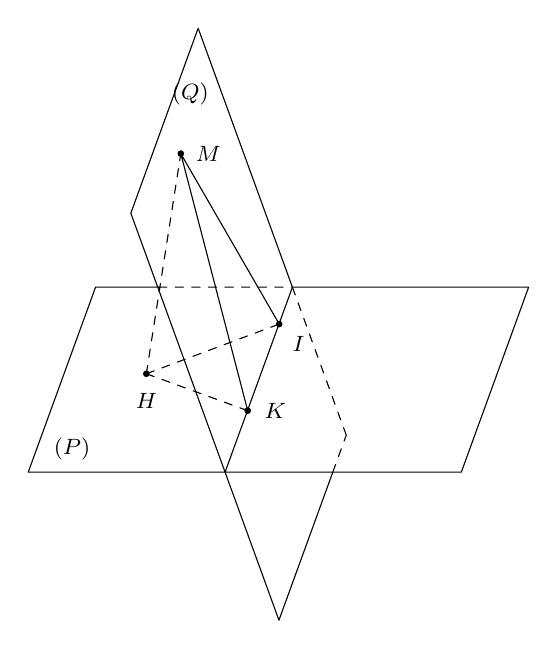
\begin{tikzpicture}[scale=1,line join=round,line cap=round,font=\footnotesize,>=stealth]% coordinates
				\path (0,0) coordinate (A) 
				++(0:2.5) coordinate (A')
				++(0:3) coordinate (B) 
				++(70:2.5)  coordinate (C)
				++(-180:3) coordinate (D)
				++(110:3.5) coordinate (R)
				++(-110:2.5) coordinate (S)
				++(-70:5.5) coordinate (T)
				++(70:2) coordinate (U)
				++(70:0.5) coordinate (W);
				\path (1.5,1.25) coordinate (H) 
				++(-20:1.37) coordinate (K) 
				++(70:1.17)  coordinate (I)
				++(120:2.5) coordinate (M);
				\path (0,0) coordinate (A)
				++(70:2.5) coordinate (E)
				++(0:0.8) coordinate (F);
				\coordinate (P) at (0.2,0.3);
				\coordinate (Q) at (1.7,4.8);
				\draw (A)--(A')--(B)--(C)--(D) (I)--(M)--(K) (A')--(D) (D)--(R)--(S)--(T)--(U) (A)--(E)--(F) ;
				\draw[dashed] (H)--(K) (H)--(I) (H)--(M) (F)--(D) (U)--(W) (D)--(W);
				\foreach \x/\y in {H/-90,K/0,I/-45,M/0 %hiện điểm
				}{\draw[fill=black] (\x) circle(1pt)++(\y:0.35)node{$\x$};}%nút tròn ngay điểm
				\path (P)node [right]{$(P)$};
				\path (Q)node [right]{$(Q)$};
			\end{tikzpicture}
		\end{center}	
		Gọi $I$ là giao điểm của đường thẳng $d$ với mặt phẳng $(P)$ và lấy điểm $M \in d,\, M \ne I$.\\
		Gọi $H$, $K$ lần lượt là hình chiếu của $M$ lên $(P)$ và giao tuyến $\Delta$ của $(P)$ và $(Q)$.\\
		Đặt $\alpha$ là góc giữa $(P)$ và $(Q)$, ta có $\alpha = \widehat{MKH}$, do đó $\tan \alpha =\dfrac{HM}{HK} \ge \dfrac{HM}{HI}$.\\
		Do đó $(Q)$ là mặt phẳng đi qua $d$ và vuông góc với mặt phẳng $(MHI)$, nên $(Q)$ đi qua $M$ và nhận $[[\overrightarrow{n}_P,\overrightarrow{u}_d],\overrightarrow{u}_d]$ làm vectơ pháp tuyến.
		\item \textbf{Cách 2: Phương pháp đại số}\\
		Ta có thể giải bài toán trên bằng phương pháp đại số như sau:\\
		\begin{itemize}
			\item Gọi $\overrightarrow{n}_Q=(a;b;c)$, $(a^2+b^2+c^2 \ne 0)$ là một vectơ pháp tuyến của mặt phẳng $(Q)$.
			\item Khi đó $\overrightarrow{n}_Q \cdot \overrightarrow{u}_d=0$ từ đây ta rút ra được $a$ theo $b$, $c$ (hoặc $b$ theo $a$, $c$ hoặc $c$ theo $a$, $b$).
			\item Gọi $\alpha$ là góc giữa $(P)$ và $(Q)$, ta có $\cos \alpha =\dfrac{|\overrightarrow{n} \cdot \overrightarrow{n}_P|}{|\overrightarrow{n}| \cdot |\overrightarrow{n}_P|}=f(t)$\\
			với $t=\dfrac{b}{c}$, $c \ne 0$. Khảo sát $f(t)$ ta tìm được $\max$ của $f(t)$.
		\end{itemize}
	\end{itemize}
	\begin{note}
		Để tìm vectơ pháp tuyến $\overrightarrow{n}_Q$ của mặt phẳng $(Q)$ đơn giản hơn thì nên gọi $\overrightarrow{n}_Q=(1;b;c)$.
	\end{note}
	
	\subsubsection{Bài toán 2}
	Trong KG $Oxyz$, cho hai đường thẳng $d$ và $d'$ chéo nhau. Viết phương trình mặt phẳng $(P)$ chứa $d$ và tạo với $d'$ một góc lớn nhất.\\
	\textbf{Phương pháp giải}
	\begin{itemize}
		\item \textbf{Cách 1: Phương pháp hình học}\\
		\begin{center}
			\begin{tikzpicture}% coordinates
				\path (0,0) coordinate (O) 
				++(0:6) coordinate (B) 
				++(70:2.5)  coordinate (C)
				++(-180:4) coordinate (D)
				++(-180:1.2) coordinate (E)
				++(-180:0.8) coordinate (F);
				\path (1.5,1.25) coordinate (H)
				++(0:2.5) coordinate (M)
				++(135:3) coordinate (A)
				++(-60:1.5) coordinate (K)
				($(A)!1.5!(M)$) coordinate (M') 
				($(M)!1.5!(A)$) coordinate (A')
				($(K)!2!(M)$) coordinate (M")
				($(M)!1.5!(K)$) coordinate (K");
				\path (5.5,1.25) coordinate (T) 
				++(135:4.5) coordinate (Q);
				\path (5.5,1.25) coordinate (T) 
				++(-45:1.5) coordinate (L);
				\coordinate (P) at (0.2,0.3);
				\coordinate (S) at (0.5,4);
				\coordinate (d) at (5,0.8);
				\coordinate (d') at (2.8,4);
				\draw (O)--(B)--(C)--(D) (H)--(M) (H)--(A) (M)--(A) (E)--(F) (F)--(O) (A)--(A') (M)--(M")(T)--(Q);
				\draw[dashed] (A)--(K) (M)--(K) (H)--(K)(E)--(D) (M)--(M')(K)--(K")(T)--(L);
				\foreach \x/\y in {H/-90,K/-90,A/90,M/45 %hiện điểm
				}{\draw[fill=black] (\x) circle(1pt)++(\y:0.35)node{$\x$};}%nút tròn ngay điểm
				\path (P)node [right]{$(P)$};
				\path (S)node [right]{$\Delta$};
				\path (d)node [right]{$d$};
				\path (d')node [right]{$d'$};
			\end{tikzpicture}
		\end{center}
		\begin{itemize}
			\item Trên đường thẳng $d$, lấy điểm $M$ và dựng đường thẳng $\Delta$ đi qua $M$ song song với $d$.\\
			Khi đó góc giữa $\Delta$ và $(P)$ chính là góc giữa $d$ và $(P)$.
			\item Trên đường thẳng $\Delta$, lấy điểm $A$. Gọi $H$ và $K$ lần lượt là hình chiếu của $A$ lên $(P)$ và $d$, $\alpha$ là góc giữa $\Delta$ và $(P)$.\\
			Khi đó $\alpha = \widehat{AMH}$ và $\cos \alpha =\dfrac{HM}{AM} \ge \dfrac{KM}{AM}$.\\
			Suy ra $(P)$ là mặt phẳng chứa $d$ và vuông góc với mặt phẳng $(AMK)$. Do đó $(P)$ đi qua $M$ và nhận $(\overrightarrow{u}_d \wedge \overrightarrow{u}_d) \wedge \overrightarrow{u}_d$ làm vectơ pháp tuyến.
		\end{itemize}
		\item \textbf{Cách 2: Phương pháp đại số}\\
		Ta có thể giải bài toán trên bằng phương pháp đại số như sau
		\begin{itemize}
			\item Gọi $\overrightarrow{n}_P=(a;b;c)$, $(a^2+b^2+c^2 \ne 0)$ là một VTPT của mặt phẳng $(P)$.
			\item Khi đó $\overrightarrow{n}_p \cdot \overrightarrow{u}_d=0$ từ đây ta rút ra được $a$ theo $b$, $c$ (hoặc $b$ theo $a$, $c$ hoặc $c$ theo $a$, $b$).
			\item Gọi $\alpha$ là góc giữa $(P)$ và $d$, ta có $\sin \alpha = \dfrac{|\overrightarrow{n} \cdot \overrightarrow{u}_d|}{|\overrightarrow{n}| \cdot |\overrightarrow{u}_d|}=f(t)$\\
			với $t=\dfrac{b}{c}$, $c \ne 0$. Khảo sát $f(t)$ ta tìm được $\max$ của $f(t)$.
		\end{itemize}
		\begin{note}
			Để tìm vectơ pháp tuyến $\overrightarrow{n}_P$ của mặt phẳng $(P)$ đơn giản hơn thì nên gọi $\overrightarrow{n}_P=(1;b;c)$.
		\end{note}
	\end{itemize}
\end{dang}
\Closesolutionfile{ans}
\Opensolutionfile{ans}[ans/ans-0-B15-KQ]
\TN
\begin{ex}%[2H5C1-5]
	Trong KG $Oxyz$, cho đường thẳng $d \colon \dfrac{x}{1}=\dfrac{y+1}{-2}=\dfrac{2-z}{1}$. Gọi $(P)$ là mặt phẳng chứa đường thẳng $d$ và tạo với mặt phẳng $(Q) \colon 2x-y-2z-2=0$ một góc có số đo nhỏ nhất. Điểm $A(1;2;3)$ cách mặt phẳng $(P)$ một khoảng bằng
	\choice
	{\True $\sqrt{3}$}
	{$\dfrac{5\sqrt{3}}{3}$}
	{$\dfrac{7\sqrt{11}}{11}$}
	{$\dfrac{4\sqrt{3}}{3}$}
	\loigiai{
		\begin{center}
			\begin{tikzpicture}% coordinates
				\path (0,0) coordinate (O) 
				++(0:6) coordinate (K) 
				++(60:3)  coordinate (P)
				++(-180:3.5) coordinate (Q)
				++(-180:1.1) coordinate (R)
				++(-180:1.4) coordinate (T);
				\path (4,4) coordinate (M)
				++(-77:2.5) coordinate (H)
				++(-180:2.5) coordinate (B)
				++(-40:1.5) coordinate (C)
				++(60:1.3) coordinate (H)
				($(C)!1.5!(B)$) coordinate (C') 
				($(B)!1.5!(C)$) coordinate (B');
				\coordinate (d) at (3.8,0.3);
				\draw (O)--(K)--(P)--(Q) (B)--(C)(H)--(C)(H)--(M)(B)--(C') (B')--(C)(B)--(M)(M)--(C)(R)--(T)(T)--(O);
				\draw[dashed] (H)--(B)(Q)--(R) ;
				\foreach \x/\y in {H/0,B/-180,C/-90,M/90 %hiện điểm
				}{\draw[fill=black] (\x) circle(1pt)++(\y:0.35)node{$\x$};}%nút tròn ngay điểm
				\path (d)node [right]{$\Delta$};
				\draw pic[draw, angle radius=2.5mm]{right angle=H--C--B'};
				\draw pic[draw, angle radius=2.5mm]{right angle=B--C--M};
				\draw pic[draw, angle radius=2.5mm]{right angle=M--H--C}; 
				\draw pic[draw, angle radius=2.5mm]{right angle=M--H--B};   
			\end{tikzpicture}
		\end{center}
		Ta có $d \colon \dfrac{x}{1}=\dfrac{y+1}{-2}=\dfrac{2-z}{1}$ có VTCP $\overrightarrow{u}=(1;-2;-1)$.\\
		$(Q) \colon 2x-y-2z-2=0$ có VTPT $\overrightarrow{n}=(2;-1;-2)$.\\
		Gọi $\alpha$ là góc tạo bởi $d$ và $(Q)$, ta có $\sin \alpha =\left|\cos(\overrightarrow{u},\overrightarrow{n})\right|=\dfrac{\sqrt{6}}{3}$.\\
		Từ hình vẽ, ta có $(d,(P))=\widehat{MBH}$ và $((P),(Q))=\widehat{MCH}$.\\
		Ta thấy $\sin \widehat{MCH}=\dfrac{MH}{MC} \ge \dfrac{MH}{MB}=\dfrac{\sqrt{6}}{3}$.\\
		Vậy góc $((P),(Q))=\widehat{MCH}$ nhỏ nhất khi $\sin \widehat{MCH}=\dfrac{\sqrt{6}}{3}$ hay $\cos \widehat{MCH}=\dfrac{\sqrt{3}}{3}$.\\
		Viết phương trình mặt phẳng $(P)$\\
		\begin{itemize}
			\item \textbf{Cách 1}\\
			Mặt phẳng $(P) \colon Ax+By+Cz+D=0$.\\
			Ta có $\heva{&\overrightarrow{n}_(Q) \cdot \overrightarrow{u}=0\\ &\cos(\overrightarrow{n},\overrightarrow{n}_(Q))=\dfrac{\sqrt{3}}{3}} 
			\Leftrightarrow \heva{&A-2B-C=0\\ &\dfrac{|2A-B-2C|}{3\sqrt{A^2+B^2+C^2}}=\dfrac{\sqrt{3}}{3}}\\
			\Leftrightarrow \heva{&A=2B+C\\ &|3B|=\sqrt{3(2B+C)^2+B^2+C^2}} \Leftrightarrow \heva{&A=2B+C\\ &6B^2+6C^2+12BC=0. \qquad(1).}$\\
			Nếu $B=0$ suy ra $A=C=0$ loại.\\
			Nếu $B\ne 0$ từ $(1)$ suy ra $\left( \dfrac{C}{B}\right) ^2+2\dfrac{C}{B}+1=0 \Leftrightarrow \dfrac{C}{B}=-1 \Rightarrow C=-B$ suy ra $A=B$.\\
			Mặt phẳng $(P) \colon Bx+By-Bz+D=0$ đi qua điểm $N(0;-1;2) \in d$ suy ra $D=3B$.\\
			Vậy phương trình mặt phẳng $(P) \colon x+y-z+3=0$. Suy ra $d(A;(P))=\sqrt{3}$.
			\item \textbf{Cách 2}\\
			Gọi $\Delta=(P) \cap (Q)$ thì góc giữa $(P)$ và $(Q)$ nhỏ nhất khi và chỉ khi $\Delta \perp d$.\\
			Do đó, mặt phẳng $(P)$ thỏa đề bài là mặt phẳng chứa $d$ và cắt $(Q)$ theo giao tuyến $\Delta$ sao cho $\Delta \perp d$.\\
			$\heva{&\Delta \subset (Q)\\ &\Delta \perp d} \Rightarrow \Delta$ nhận $\overrightarrow{u}_\Delta=\left[ \overrightarrow{u}_d,\overrightarrow{n}_(Q)\right] $ làm vectơ chỉ phương.\\
			$(Q)$ chứa $d$ và $\Delta$ $\Rightarrow (P)$ qua $M(0;-1;2) \in d$ và nhận $\overrightarrow{n}=\left[ \overrightarrow{u}_d,\overrightarrow{u}_\Delta\right] =(6;6;-6)$ làm vectơ pháp tuyến $\Rightarrow(P) \colon x+y-z+3=0$.\\
			Vậy $d(A;(P))=\sqrt{3}$.
		\end{itemize}
	}
\end{ex}
%%--------------- 
\begin{ex}%[GVBS: Mai Trung Hiếu]%[2H5V2-7]
	Trong KG $Oxyz$, cho đường thẳng $\Delta \colon \dfrac{x}{2}=\dfrac{y}{2}=\dfrac{z}{1}$ và mặt phẳng $(P): x+2 y-2 z=0$.
	Gọi $(Q)$ là mặt phẳng chứa $\Delta$ sao cho góc giữa hai mặt phẳng $(P)$ và $(Q)$ là nhỏ nhất. Phương trình mặt phẳng $(Q)$ là
	\choice
	{$x-2 y+z=0$}
	{$x+22 y+10 z=0$}
	{$x-2 y-z=0$}
	{\True $x+10 y-22 z=0$}
	\loigiai{
		\begin{center}
			\begin{tikzpicture}[
				>=stealth, line join=round, line cap=round, 
				scale=.8,
				font=\footnotesize,
				declare function={r=3; a=75;}]
				% ve diem
				\path 
				(0,0) coordinate (a)
				(2,4) coordinate (b)
				(10,4) coordinate (c)
				(8,0) coordinate (d)
				(4,6) coordinate (e)
				(6,10) coordinate (f)
				(6.5,6) coordinate (B)
				(8.5,1) coordinate (A)
				(9.5,3) coordinate (K)
				(6.5,3) coordinate (H)
				(intersection of b--c and e--d) coordinate (g)
				;
				\draw[thick] 
				(a)--(d)--(c)--(f)--(e)--(d)
				(a)--(b)--(g)
				(K)--(B)
				;
				\draw[thick, shorten >=-1cm, shorten <=-1cm]
				(B)--(A) node[pos=-.2, above right] {$\Delta$}
				;
				\draw[dashed]
				(c)--(g)
				(K)--(H)--(A)
				(B)--(H)
				;
				% danh dau goc
				\foreach \a/\b/\c in {c/K/b, K/H/B}	{
					\draw pic [draw=black,angle radius = 6] {right angle = \a--\b--\c};
				}
				%	\draw pic ["$1$", draw, angle eccentricity=1.3, angle radius=20] {angle = B--A--C};
				% danh dau diem
				\foreach \x/\g in {A/0, B/45, K/0, H/135}{
					\draw[fill=black] (\x) circle (1.5pt)+(\g:.4) node{$\x$};}
				\node[above right] at (a) {$P$};
				\node[below] at (f) {$Q$};
				\node[right] at (9,2) {$d$};
			\end{tikzpicture}
		\end{center}
		Đường thẳng $\Delta \colon \dfrac{x}{2}=\dfrac{y}{2}=\dfrac{z}{1}$ được viết lại dưới dạng tham số $\Delta \colon \heva{&x=2 t \\ &y=2 t \\ &z=t.}$
		\\
		Xét hệ phương trình
		$$
		\heva{&x=2 t \\ &y=2 t \\ &z=t \\ &x+2 y-2 z=0}
		\Leftrightarrow
		\heva{&t=0 \\ &x=0 \\ &y=0 \\ &z=0.}
		$$
		Do đó $\Delta$ cắt $(P)$ tại điểm $A(0 ; 0 ; 0) \equiv O$.
		\\
		Lại có $\Delta$ và $(P)$ không vuông góc nhau nên ta đi chứng minh góc nhỏ nhất giữa $(P)$ và $(Q)$ là góc giữa $\Delta$ và $(P)$. Thật vậy trên $\Delta$ lấy $B$ khác $A$, kẻ $BH$ vuông góc với $(P)$ tại $H$ và $B K$ vuông góc $d$ tại $K$ ($d$ là giao tuyến của $(P)$ và $(Q)$) tại $K$. Khi đó góc giữa $(Q)$ và $(P)$ là góc $BKH$.
		Ta thấy
		$$
		HA \geq HK 
		\Rightarrow 
		\tan \widehat{BKH}=\dfrac{BH}{HK}
		\geq
		\dfrac{BH}{HA}=\tan \widehat{BAH}.
		$$
		Mà $\widehat{BKH}$, $\widehat{BAH}<90^{\circ}$ nên
		$$
		\widehat{BKH} \geq \widehat{BAH}=(\Delta,(P))=\arcsin \dfrac{4}{9}.
		$$
		Đẳng thức xảy ra $\Leftrightarrow K \equiv A \Leftrightarrow \Delta \perp d$.
		\\
		Do đó, góc giữa hai mặt phẳng $(P)$ và $(Q)$ là nhỏ nhất khi và chỉ khi $(Q)$ chứa $(\Delta)$ và cắt $(P)$ theo một giao tuyến vuông góc $\Delta$.
		\\
		*Viết phương trình của $(Q)$
		\\
		Đường thẳng $\Delta$ có vec-tơ chỉ phương $\vec{u_1}=(2 ; 2 ; 1)$, $(P)$ có vec-tơ pháp tuyến $\vec{n_1}=(1 ; 2 ;-2)$ nên $d$ có vec-tơ chỉ phương $\vec{u_2}=\left[\vec{u_1}, \vec{n_1}\right]=(-6 ; 5 ; 2)$.
		\\
		$(Q)$ chứa $\Delta$ và $d$ nên nhận $\vec{n_2}=\left[\vec{u_2} ; \vec{u_1}\right]=(1 ; 10 ;-22)$ làm vec-tơ pháp tuyến.
		\\
		Vậy mặt phẳng $(Q)$ đi qua $A(0 ; 0 ; 0)$ và nhận $\vec{n_2}=(1 ; 10 ;-22)$ làm vec-tơ pháp tuyến nên có phương trình $x+10 y-22 z=0$.
	}
\end{ex}

%%--------------- 
\begin{ex}%[GVBS: Mai Trung Hiếu]%[2H5V2-7]
	Trong KG $Oxyz$, cho đường thẳng $d: \dfrac{x}{-1}=\dfrac{y+1}{2}=\dfrac{z-2}{1}$ và mặt phẳng $P \colon 2 x-y-2 z-2=0$.
	$(Q)$ là mặt phẳng chứa $d$ và tạo với $(P)$ một góc nhỏ nhất. Gọi $\vec{n}_Q=a ; b ; 1$ là một vec-tơ pháp tuyến của $(Q)$. Đẳng thức nào đúng?
	\choice
	{$a-b=-1$}
	{\True $a+b=-2$}
	{$a-b=1$}
	{$a+b=0$}
	\loigiai{
		Đường thẳng $d$ đi qua điểm $M (0 ;-1 ; 2)$ và có vec-tơ chỉ phương $\vec{u_d}=(-1 ; 2 ; 1)$.
		\\
		Theo giả thiết, $d \subset (Q)$ và $\vec{n}_Q=(a ; b ; 1)$ là một vec-tơ pháp tuyến của $Q$ nên ta có
		$$
		\vec{u_d} \cdot \vec{n}_Q=0 \Leftrightarrow-a+2 b+1=0 \Leftrightarrow a=2 b+1 \quad (1).
		$$
		Mặt phẳng $(P)$ có vec-tơ pháp tuyến $\vec{n}_P=(2 ;-1 ;-2)$.
		\\
		Ta có
		$$
		\cos \left((P), (Q)\right)=\left|\cos \left(\vec{n}_P, \vec{n}_Q\right)\right|=\dfrac{|2 a-b-2|}{3 \cdot \sqrt{a^2+b^2+1}} \quad (2).
		$$
		Thế (1) vào (2), ta được $\cos \left((P), (Q)\right)=\dfrac{|b|}{\sqrt{5 b^2+4 b+2}}$.
		\\
		Khi góc giữa $(P)$ và $(Q)$ nhỏ nhất thì $\cos \left((P), (Q)\right)$ đạt giá trị lớn nhất.
		\\
		Xét hàm số $f(b)=\dfrac{b}{\sqrt{5 b^2+4 b+2}}$, có
		$$
		f'(b)=\dfrac{b+1}{\sqrt{5 b^2+4 b+2}}=0 \Leftrightarrow b=-1.
		$$
		Bảng biến thiên
		\begin{center}
			
\begin{tikzpicture}
				\tkzTabInit[lgt=2,espcl=4,deltacl=0.6]
				{$b$/1, $f'(b)$/1, $f(b)$/2}
				{$-\infty$, $-1$, $+\infty$}
				\tkzTabLine{, -, z, +}
				\tkzTabVar{+/$-\dfrac{1}{\sqrt{5}}$, -/$-\dfrac{1}{\sqrt{3}}$, +/$\dfrac{1}{\sqrt{5}}$}
			\end{tikzpicture}
		\end{center}
		Từ đó suy ra với hàm số $g(b)=\dfrac{|b|}{\sqrt{5 b^2+4 b+2}}$ có
		$$
		\max\limits_{\mathbb{R}} g(b)=g(-1)=-\dfrac{1}{\sqrt{3}}.
		$$ 
		Khi $b=-1 \Rightarrow a=-1$.
		\\
		Vậy, $a+b=-2$.
	}
\end{ex}
\Closesolutionfile{ans}
\indapan{6}{ans/ans-0-B15-KQ}